\documentclass[a4paper, twoside, openright]{report}

% some page formatting packages
\linespread{1.3} % line spacing for when it becomes necessary
\usepackage{parskip}
\usepackage[inner=3cm, outer=2cm, bottom=2cm]{geometry}
\usepackage{lscape}
\pagestyle{headings}
\usepackage{microtype} % prettyfication
\usepackage{emptypage} % remove headers from empty pages

\makeatletter
\renewcommand{\maketitle}
{
	\begin{titlepage}
		\begin{center}
			\includegraphics[width=0.15\textwidth]{Images/BCU.jpg} \\
			\vspace{0.5em}
			{\huge Digital Media Technology Lab} \\
			\vspace{0.5em}
			{\huge Birmingham City University} \\
			\vspace{14em}
			{\bfseries \Huge \@title} \\
			\vspace{3em}
			{\huge \@author} \\
			\vspace*{\fill}
			{\Large A thesis submitted in partial fulfilment of the requirements for the degree of Doctor of
			Philosophy, \@date}
		\end{center}
	\end{titlepage}
}
\makeatother

% abstract stuff
\renewenvironment{abstract}
{
	\cleardoublepage
	\phantomsection
	\addcontentsline{toc}{chapter}{Abstract}
	\thispagestyle{plain}
	\setcounter{page}{1}
	\vspace*{\fill}
	\begin{center}
		{\bfseries \Large Abstract}
	\end{center}
}
{
	\vspace*{\fill}
}

% acknowledgements stuff
\newenvironment{acknowledgements}
{
	\cleardoublepage
	\phantomsection
	\addcontentsline{toc}{chapter}{Acknowledgements}
	\thispagestyle{plain}
	\vspace*{\fill}
	\begin{center}
		{\bfseries \Large Acknowledgements}
	\end{center}
}
{
	\vspace*{\fill}
}

% packages for figures
\usepackage[pdftex]{graphicx}
\usepackage{subfig}
\usepackage[justification=centering]{caption}
\usepackage{epstopdf}

% data float type
\usepackage{float}
\newfloat{datum}{htbp}{lod}[chapter]
\floatname{datum}{Datum}
\newsubfloat{datum}

% oh yes we have to use Harvard referencing or Peter will kill us
\usepackage{natbib}
\usepackage{bibentry}
\nobibliography*

% packages for the formatting of equations
\usepackage{amsmath}
\DeclareMathOperator{\sgn}{sgn}
\newcommand{\floor}[1]{\left\lfloor#1\right\rfloor}
\newcommand{\ceil}[1]{\left\lceil#1\right\rceil}
\newcommand{\round}[1]{\left\lfloor#1\right\rceil}
\newcommand{\abs}[1]{\left|#1\right|}
\newcommand{\euclidian}[1]{\left|\left|#1\right|\right|}
\newcommand{\medcap}{\mathbin{\raisebox{\depth}{\scalebox{0.75}{\ensuremath{\bigcap}}}}}
\newcommand{\medcup}{\mathbin{\raisebox{\depth}{\scalebox{0.75}{\ensuremath{\bigcup}}}}}
\usepackage{amsfonts}
\usepackage{mathabx}

% make some colours and commands so we can put in notes to ourself
\usepackage{color}
\definecolor{noteColour}{RGB}{0, 0, 255}
\definecolor{todoColour}{RGB}{255, 0, 0}
\newcommand{\note}[1]{{\color{noteColour}#1}}
\newcommand{\todo}[1]{{\color{todoColour}#1}}

% sub/superscript commands
\newcommand{\sub}[1]{\textsubscript{#1}}
\newcommand{\super}[1]{\textsuperscript{#1}}

% clickable links for references in the document also put page cited on info in the bibliography
\usepackage[backref=page]{hyperref}
\hypersetup
{
	colorlinks,
	citecolor=black,
	filecolor=black,
	linkcolor=black,
	urlcolor=black
}
\renewcommand*{\backref}[1]{}
\renewcommand*{\backrefalt}[4]
{
	\ifcase #1 [Not Cited.]
	\or [Cited on Page #2.]
	\else [Cited on Pages #2.]
	\fi
}

% gotta draw them diagrams in tikz, otherwise you fail at life
\usepackage{tikz}
\usetikzlibrary{fit, arrows, shapes, patterns, positioning}
\tikzstyle{dots} = [dotted]
\tikzstyle{operator} = [circle, draw=black]
\tikzstyle{gain} = [regular polygon, regular polygon sides=3, inner sep=0, draw=black, shape border rotate=270,
                    minimum size=2em]

% fuck serifs
\renewcommand{\familydefault}{\sfdefault}

% make those tables pretty
\usepackage{array}
\usepackage{hhline}
\newcolumntype{C}[1]{>{\centering}p{#1}}

% appendices :(
\usepackage[toc]{appendix}

% glossary options
\usepackage[acronym, nonumberlist, nomain, toc, style=super]{glossaries}
\newglossary[mlg]{maths}{mni}{mno}{Mathematical Notation}
\setlength{\glsdescwidth}{0.8\textwidth}
\makeglossaries

% glossary entries
\newacronym{adsr}{ADSR}{Attack, Decay, Sustsain, Release}
\newacronym{dft}{DFT}{Discrete Fourier Transform}
\newacronym{dct}{DCT}{Discrete Cosine Transform}
\newacronym{stft}{STFT}{Short-Time Fourier Transform}
\newacronym{mfccs}{MFCCs}{Mel Frequency Cepstral Coefficients}
\newacronym{mds}{MDS}{Multidimensional Scaling}
\newacronym{pca}{PCA}{Principal Component Analysis}
\newacronym{pc}{PC}{Principal Component}
\newacronym{efa}{EFA}{Exploratory Factor Analysis}
\newacronym{lti}{LTI}{Linear Time Invariant}
\newacronym{ltv}{LTV}{Linear Time Variant}
\newacronym{thd}{THD}{Total Harmonic Distortion}
\newacronym{imd}{IMD}{Intermodulation Distortion}
\newacronym{ssba}{SSBA}{Single Sideband Automodulation}
\newacronym{iap}{IAP}{Instantaneous Amplitude and Phase}
\newacronym{sttr}{STTR}{Short-Time Time Reversal}
\newacronym{daw}{DAW}{Digital Audio Workstation}
\newacronym{fir}{FIR}{Finite Impulse Response}
\newacronym{iir}{IIR}{Infinte Impulse Response}
\newacronym{vame}{VAME}{Verbal Attribute Magnitude Estimation}
\newacronym{mushra}{MUSHRA}{Multiple Stimuli with Hidden Reference and Anchor}
\newacronym{api}{API}{Application Programming Interface}
\newacronym{safe}{SAFE}{Semantic Audio Feature Extraction}
\newacronym{lfo}{LFO}{Low Frequency Oscillator}
\newacronym{erb}{ERB}{Equivalent Rectangular Bandwidth}
\newacronym{vst}{VST}{Virtual Studio Technology}
\newacronym{au}{AU}{Audio Unit}
\newacronym{rdf}{RDF}{Resource Description Framework}
\newacronym{eq}{EQ}{Equaliser}
\newacronym{amdf}{AMDF}{Average Magnitude Difference Function}
\newacronym{hps}{HPS}{Harmonic Product Spectrum}

\newglossaryentry{maths:round}
{
	type=maths,
	name={$\round{a}$},
	description={$a$ rounded to the nearest integer},
	sort={round}
}
\glsadd{maths:round}

\newglossaryentry{maths:divides}
{
	type=maths,
	name={$a \divides b$},
	description={$a$ divides $b$, i.e. $\dfrac{b}{a}$ is an integer.},
	sort={divides}
}
\glsadd{maths:divides}

\newglossaryentry{maths:signum}
{
	type=maths,
	name={$\sgn(a)$},
	description={the signum funciton (the sign of $a$), $1$ for $a > 0$, $-1$ for $a < 0$, $0$ for $a = 0$},
	sort={fsignum}
}
\glsadd{maths:signum}

\newglossaryentry{maths:max}
{
	type=maths,
	name={$\displaystyle \max_{i = 0}^{I} A_{i}$},
	description={the maximum value of $A_{i}$ for $0 \leq i \leq I$},
	sort={max}
}
\glsadd{maths:max}

\newglossaryentry{maths:euclidian}
{
	type=maths,
	name={$\euclidian{a - b}$},
	description={the Euclidian distance between points $a$ and $b$ in a multidimensional space},
	sort={euclidian}
}
\glsadd{maths:euclidian}

\newglossaryentry{maths:setcomp}
{
	type=maths,
	name={$A \setminus B$},
	description={the relative complement of set $B$ with respect to set $A$ (the set of elements in $A$ which are not in
		     $B$)},
	sort={setcomp}
}
\glsadd{maths:setcomp}

\newglossaryentry{maths:subset}
{
	type=maths,
	name={$A \subseteq B$},
	description={$A$ is a subset of or equal to $B$ ($A$ only contain elements which are also in $B$)},
	sort={subset}
}
\glsadd{maths:subset}

\newglossaryentry{maths:setunion}
{
	type=maths,
	name={$A \protect\medcup B$},
	description={the union of sets $A$ and $B$ (the set which contains all elements in both $A$ and $B$)},
	sort={setunion}
}
\glsadd{maths:setunion}

\newglossaryentry{maths:setmembership}
{
	type=maths,
	name={$a \in A$},
	description={set membership, $a$ is an element of $A$},
	sort={setmembership}
}
\glsadd{maths:setmembership}

\newglossaryentry{maths:thenaturalnumbers}
{
	type=maths,
	name={$\textbf{N}$},
	description={the set of all natural numbers (integers greater than zero)},
	sort={thenaturalnumbers}
}
\glsadd{maths:thenaturalnumbers}

\newglossaryentry{maths:theintegers}
{
	type=maths,
	name={$\textbf{Z}$},
	description={the set of all integers},
	sort={theintegers}
}
\glsadd{maths:theintegers}

\author{Sean Enderby}
\title{Timbral Control of Audio Through Harmonic Excitation}
\date{November 2017} % fill that shit in when i'm done

\begin{document}

\pagenumbering{roman}
\maketitle

\begin{center}
	\includegraphics[width=0.8\textwidth]{Images/seanFace.jpg}
	\newline
	\newline
	\Huge
	Welcome to my thesis, are your ready for some fun?
	\normalsize
\end{center}

\tableofcontents

\pagenumbering{arabic}
%\setcounter{chapter}{0}
\chapter{Introduction}
\label{chap:Introduction}

\section{Motivation}
\label{sec:Introduction-Motivation}
% Genuine Waffle (if those who disagree have uncovered this comment I have no regrets)
	The process of music production can be split into four main stages (recording, editing, mixing and mastering) as
	shown in Figure~\ref{fig:MusicProduction}. In the recording stage, acoustic and digital sound sources are captured
	resulting in a set of recorded audio signals (often called stems). These are then edited to correct any mistakes
	made during the recording and to arrange them in time, forming the musical structure of the finished piece. The
	signals are then processed further and mixed together to produce the final product.

	\begin{figure}[h!]
		\centering
		\begin{tikzpicture}
			\node (Sources) [align=center] at (0, 0) {Sound\\Sources};
			\node (Mic1) [draw] at (2, 1.5) {Microphone};
			\node (Mic2) [draw] at (2, 0.5) {Microphone};
			\node (Mic3) [draw] at (2, -0.5) {Microphone};
			\node (Mic4) [draw] at (2, -1.5) {Microphone};

			\draw [dots] (3.2, 3) -- (3.2, -2);
			\node (Recording) at (2, 2.5) {\bf{Recording}};

			\node (Edit1) [draw] at (4.5, 1.5) {Editing Tools};
			\node (Edit2) [draw] at (4.5, 0.5) {Editing Tools};
			\node (Edit3) [draw] at (4.5, -0.5) {Editing Tools};
			\node (Edit4) [draw] at (4.5, -1.5) {Editing Tools};

			\draw (Mic1) -- (Edit1);
			\draw (Mic2) -- (Edit2);
			\draw (Mic3) -- (Edit3);
			\draw (Mic4) -- (Edit4);

			\draw [dots] (5.8, 3) -- (5.8, -2);
			\node (Editing) at (4.5, 2.5) {\bf{Editing}};

			\node (Proc1) [draw] at (6.9, 1.5) {Processing};
			\node (Proc2) [draw] at (6.9, 0.5) {Processing};
			\node (Proc3) [draw] at (6.9, -0.5) {Processing};
			\node (Proc4) [draw] at (6.9, -1.5) {Processing};

			\draw (Edit1) -- (Proc1);
			\draw (Edit2) -- (Proc2);
			\draw (Edit3) -- (Proc3);
			\draw (Edit4) -- (Proc4);

			\node (Mixer) at (9.1, 0) {Mixer};
			\draw (8.2, 1.8) rectangle (10, -1.8);
			\coordinate (Mix1) at (8.2, 1.5);
			\coordinate (Mix2) at (8.2, 0.5);
			\coordinate (Mix3) at (8.2, -0.5);
			\coordinate (Mix4) at (8.2, -1.5);

			\node (Mixing) at (8, 2.5) {\bf{Mixing}};

			\draw (Proc1) -- (Mix1);
			\draw (Proc2) -- (Mix2);
			\draw (Proc3) -- (Mix3);
			\draw (Proc4) -- (Mix4);

			\draw [dots] (10.2, 3) -- (10.2, -2);
			\node (Mastering) at (11.3, 2.5) {\bf{Mastering}};

			\node (Master) [draw] at (11.3, 0) {Processing};
			\draw (10, 0) -- (Master);

			\node (Mix) [align=center] at (13.2, 0) {Finished\\Product};
			\draw (Master) -- (Mix);
		\end{tikzpicture}
		\caption{A block diagram of the music production process.}
		\label{fig:MusicProduction}
	\end{figure}

	During the mixing and mastering stages, audio effects are used to creatively shape the timbre of recorded audio
	signals. This is represented by the blocks labelled ``Processing'' in Figure~\ref{fig:MusicProduction}. This allows
	producers to create timbres which are not possible to achieve through only the recording of acoustic instruments.
	Traditional audio effects evolved from the use of analogue signal processing systems designed to address the
	technical requirements of broadcast or recording. As such, these effects have control parameters which relate
	directly to specific technical properties of an audio signal: a traditional equaliser has parameters for selecting
	specific frequency regions, traditional dynamics processors (compressors and limiters) have parameters relating to
	signal amplitudes. These parameters are effective when correcting technical issues with a signal but do not allow
	for intuitive creative manipulation of timbre.

	The application of audio effects for creative purposes is typically motivated by the perceived timbre of the audio.
	Creative decisions are often expressed using language which does not refer to the mathematical properties of the
	recorded signals. For example, one might ask that the saxophone is made more present in the mix, or that the piano
	be made to sound more airy. In order to complete these tasks using traditional audio effects, music producers and
	audio engineers require knowledge of how the technical parameters of the effect relate to specific perceived aspects
	of timbre. This knowledge is gained through training and experience, presenting an obstacle to novices.

	Audio production software typically uses parameter presets to assist novice users. These are a predefined set of
	parameter values for a particular effect which are labelled with semantic descriptions. Users can apply an effect to
	a signal and choose a preset which best fits their desired outcome. This does not, however, provide an intuitive
	interface to the user. A static parameter setting will not apply the same timbral transformation to all input
	signals. If the user wishes to alter the settings slightly, they still require knowledge of how the effect's
	parameters relate to perceived timbre. For example, a user might apply a preset to make a sound brighter, if they
	are not happy with the result no assistance is given in making the sound more or less bright.

	More intuitive interfaces for control over timbre provide parameters which directly relate to perceived aspects of a
	sound. These perform the translation between the language used to describe timbre and the technical parameters of
	signal processing algorithms, allowing users to focus on the creative aspects of music production. Having timbral
	properties controlled by continuous parameters increases the intuitiveness of the system as it is evident which
	parameter to adjust to change a particular timbral property. The effect can also analyse the input signal and adjust
	itself such that the parameter has similar timbral effects across a wide range of inputs. Developing this type of
	semantically controlled effect requires study of how the mathematical properties of a signal contribute to its
	perceived timbre. Effects can then be built which manipulate these signal properties according to the value of a
	semantically labelled parameter. Making audio effects more intuitive in this manner aids both novice and experienced
	music producers and audio engineers. Novices benefit from the reduced amount of knowledge needed to apply audio
	effects; being able to select and adjust effects based on natural language descriptions of timbre rather than
	requiring a technical knowledge of signal processing. For experienced users these effects can be used to accelerate
	the production process; reducing the work required to configure audio effect parameters, allowing users to focus on
	creative decisions. 
	
	Commercial audio effects with semantically labelled parameters have been available for a number of years, for
	example the OneKnob series of effects produced by \citet{wavesoneknob}. Being commercial products, the operation of
	these effects is not known, but it is assumed that they were developed alongside input from professional audio
	engineers. In academic research, a number of studies have been undertaken in developing these types of control
	systems for synthesis and audio processing applications (discussed in Section~\ref{sec:Timbre-Control}). This work
	focusses on how this type of system can be built using nonlinear distortion / excitation effects.

\section{Objectives and Research Questions}
\label{sec:Introduction-Objectives}
	The underlying objective of this thesis is to produce intuitive timbre shaping effects based on harmonic excitation
	algorithms (systems which introduce new harmonic partials to a signal). This is achieved through answering the
	following questions:

	\begin{itemize}
		\item What semantic terms are commonly used to describe the timbre of harmonic excitation effects? 
		\item What properties of audio signals contribute to these timbral descriptions and what alterations are
		      made to signals to produce a certain timbral result?
		\item What properties of audio signals can be reliably controlled by harmonic excitation algorithms?
		\item How can harmonic excitation systems be configured to control elements of timbre? Systems will be
		      proposed which allow control over particular semantic features and the accuracy of these systems
		      assessed.
		\item Can harmonic excitation be used to provide intuitive control of timbre? Do the proposed systems
		      provide control over the aspects of timbre they are designed to?
	\end{itemize}

\section{Thesis Structure}
\label{sec:Introduction-ThesisStructure}
	The aim of this work is to develop harmonic excitation systems which provide intuitive control over timbre.
	Firstly, a review of the existing work in timbral manipulation and nonlinear processing is given. Experiments are
	then conducted to discover how spectral manipulations are used in music production. This information is used to aid
	in the design of semantically controlled harmonic excitation effects which are subsequently evaluated in perceptual
	listening tests. This is presented in seven chapters as follows:

	In {\bf{Chapter~\ref{chap:Timbre}}} the background of research into timbre is discussed. It begins with a discussion
	of the low level features of audio signals. Popular experimental methodologies for uncovering the perceptual effects
	of these features are then introduced along with the methods used to analyse their results. Finally, existing work
	concerning the control of perceptual features of audio signals is discussed.

	{\bf{Chapter~\ref{chap:Excitation}}} covers the body of work concerning harmonic excitation, starting with a
	discussion of the analysis of nonlinear systems in the field of audio production. The uses of such systems and the
	their timbral effects are then presented. Finally, various algorithms for harmonic excitation, proposed in existing
	literature, are described.

	In {\bf{Chapter~\ref{chap:TimbreEvaluation}}} the collection of semantic audio data during the music production
	process is discussed. This data is used to determine the language used for describing audio in a studio environment
	and how audio effects are used to evoke certain timbral descriptors.

	In {\bf{Chapter~\ref{chap:ExcitationEvaluation}}} a set of criteria for assessing the applicability of harmonic
	excitation techniques to timbral control is proposed. The algorithms described in Chapter~\ref{chap:Excitation} are
	then evaluated against these criteria to identify those most suitable for use in timbral control systems.  Methods
	by which the performance of certain harmonic excitation methods can be improved are proposed.

	In {\bf{Chapter~\ref{chap:FeatureControl}}}, results from Chapter~\ref{chap:ExcitationEvaluation} are used to inform
	the design of systems for controlling low level features using harmonic excitation techniques. Systems are developed
	which can be used to provide monotonic control over a specific low level feature of the input signal. The operation
	of these systems is evaluated using a number of test signals.

	In {\bf{Chapter~\ref{chap:PerceptualExperiments}}} the systems proposed in Chapter~\ref{chap:FeatureControl} are
	refined, using the results of Chapter~\ref{chap:TimbreEvaluation}, to develop harmonic excitation effects which
	control specific timbral traits of a signal. These effects are evaluated objectively, through comparison with the
	dataset gathered in Chapter~\ref{chap:TimbreEvaluation}; and subjectively, through a series of perceptual listening
	tests.

	We conclude in {\bf{Chapter~\ref{chap:Conclusion}}} with a summary of findings across Chapters
	\ref{chap:TimbreEvaluation} to \ref{chap:PerceptualExperiments}, a critique of the methods used in this work and
	suggestions for further work in this area.

\section{Contributions}
\label{sec:Introduction-Contributions}
	The primary contribution of this thesis is the proposal of methods by which harmonic excitation systems can be
	configured to give intuitive control over timbral features. In achieving this a number of other contributions are
	made, as follows:

	\begin{itemize}
		\item A new method for the collection of semantic audio descriptors and their underlying features
		      (Chapter~\ref{chap:TimbreEvaluation}).
		\item A new metric for the measurement of agreement in multidimensional distributions
		      (Chapter~\ref{chap:TimbreEvaluation}).
		\item A methodology for the assessment of harmonic generation algorithms for use in timbral control
		      (Chapter~\ref{chap:ExcitationEvaluation}).
		\item A comparison of harmonic generation algorithms and their suitability to provide perceptual control
		      (Chapter~\ref{chap:ExcitationEvaluation}).
		\item The development of new harmonic excitation systems for control of low level audio features
		      (Chapter~\ref{chap:FeatureControl}).
		\item New methods for controlling perceptual attributes using harmonic excitation
		      (Chapter~\ref{chap:PerceptualExperiments}).
	\end{itemize}

	The following papers have been published as part of this work:

	\begin{itemize}
		\item \bibentry{enderby2012harmonic}.
		\item \bibentry{enderby2013methods}.
		\item \bibentry{stables2014safe}.
		\item Enderby, S. and Stables, R. (September 2017), A Nonlinear Method for Manipulating Warmth and
		      Brightness, in \emph{Proceedings of the International Conference on Digital Audio Effects (DAFx-17)}.
	\end{itemize}

	Other associated publications include:

	\begin{itemize}
		\item Ward, D., Enderby, S., Athwal, C. and Reiss, J. (December 2015), Real-Time Excitation Based Binaural
		      Loudness Meters, in \emph{Proceedings of the International Conference on Digital Audio Effects
		      (DAFx-15)}.
		\item Stables, R., De Man, B., Enderby, S., Reiss, J., Fazekas, G. and Wilmering, T. (October 2016),
		      Semantic Description of Timbral Transformations in Music Production, in \emph{Proceedings of the
		      2016 ACM on Multimedia Conference}.
		\item Stasis, S., Jillings, N., Enderby, S. and Stables, R. (September 2017), Audio Processing Chain
		      Recommendation, in \emph{Proceedings of the International Conference on Digital Audio Effects
		      (DAFx-17)}.
	\end{itemize}

%Review of timbral control research.
%	Timbre Definition
%	Timbre Spaces (MDS and shit)
%	Audio Features
%	Perceptual Control of Synthesis

\chapter{Timbre}
\label{chap:Timbre}
	There are three properties which describe how a sound is perceived, these being loudness, pitch and timbre. Loudness
	describes the perceived intensity of a sound and pitch its perceived frequency. Timbre then describes any other
	properties of a sound, besides loudness and pitch, which allow it to be distinguished from other sounds
	\citep{mathews1999introduction}. Loudness and pitch are both one dimensional properties allowing sounds to be
	ordered from quiet to loud or low to high pitch. Timbre is a more complex property consisting of multiple dimensions
	\citep{rossing2002the}. There is a large body of research concerning the analysis of timbre, identifying these
	dimensions and their relationships with the acoustic features of a sound.

	Simple descriptions of a sounds timbre involve instrument identification. A sound could be described as `cello-like'
	or `flute-like'. More broadly the class of instrument, string or woodwind, could be used to describe the timbre of a
	sound. While these terms are useful for discussing the instrumentation of pieces they can not be applied generally
	to a wide range of timbres. It is not very useful to describe the timbre of a xylophone as being `not flute-like'.

	More general timbral descriptors directly describe the sound itself rather than the source which produced it. These
	include terms such as bright, rough and sharp. This allows the timbre of different sounds to be compared according
	to these terms \citep{howard2009acoustics}. Sounds can also be ordered in respect to these criteria much like with
	loudness and pitch. For example one could order a set of sounds by how bright they sound.

	Early research into timbre was performed by \citet{helmholtz1875on}. More recent work involves research from various
	fields. Low level features of audio segments can be found using signal analysis techniques. More complicated
	information about the perception of a signal can be discovered through modelling the behaviour of the human hearing
	system. Lastly experiments can be undertaken in which participants listen to audio samples and provide responses
	regarding the timbre of the samples. These responses are then analysed to uncover any correlations between the
	participants responses and lower level features of the audio samples.

	This chapter will review the existing body of timbral research. Section \ref{sec:Timbre-LowLevelFeatures} discusses
	metric which are used to describe the low level features of audio signals. Section
	\ref{sec:Timbre-PsychoacousticPrinciples} covers various models which describe the perception of various auditory
	phenomena. \note{Put in what the rest of the sections are about}.

\section{Low Level Audio Features}
\label{sec:Timbre-LowLevelFeatures}
	A widely cited definition of timbre \citep{ASA1960american} suggests that timbre in influenced by various low level
	features of an audio signal. The spectral content, waveform and temporal characteristics all effect the perceived
	timbre of a sound. Signal analysis techniques can be used to extract information about these elements of a signal.
	A large list of such features feature extraction techniques is given by \citep{peeters2004a}. These features can be
	separated into three categories. Features which describe the properties of a signals waveform and how it evolves
	with time (temporal features), features which describe the frequency content of a signal (spectral features) and
	features which describe how the frequency content of a signal evolves with time (spectro-temporal features). 

	\subsection{Temporal Features}
	\label{sec:Timbre-LowLevelFeatures-Temporal}
		Simple temporal features involve taking statistical measurements, such as mean and variance, of the audio
		samples in a signal. These measures give basic information about the level and variation in a signal but in
		many cases they do not represent a signals properties very well. For example, the mean value of a sinusoidal
		signal over a whole number of cycles is zero. 

		A common technique to extract more meaningful information about a signals level is to use an envelope
		detector. An envelope detector extracts the amplitude envelope of a signal. The amplitude envelope provides
		information about the level of a signal over time. An example amplitude envelope is shown in Figure
		\ref{fig:AmplitudeEnvelope}.

		\begin{figure}[h!]
			\centering
			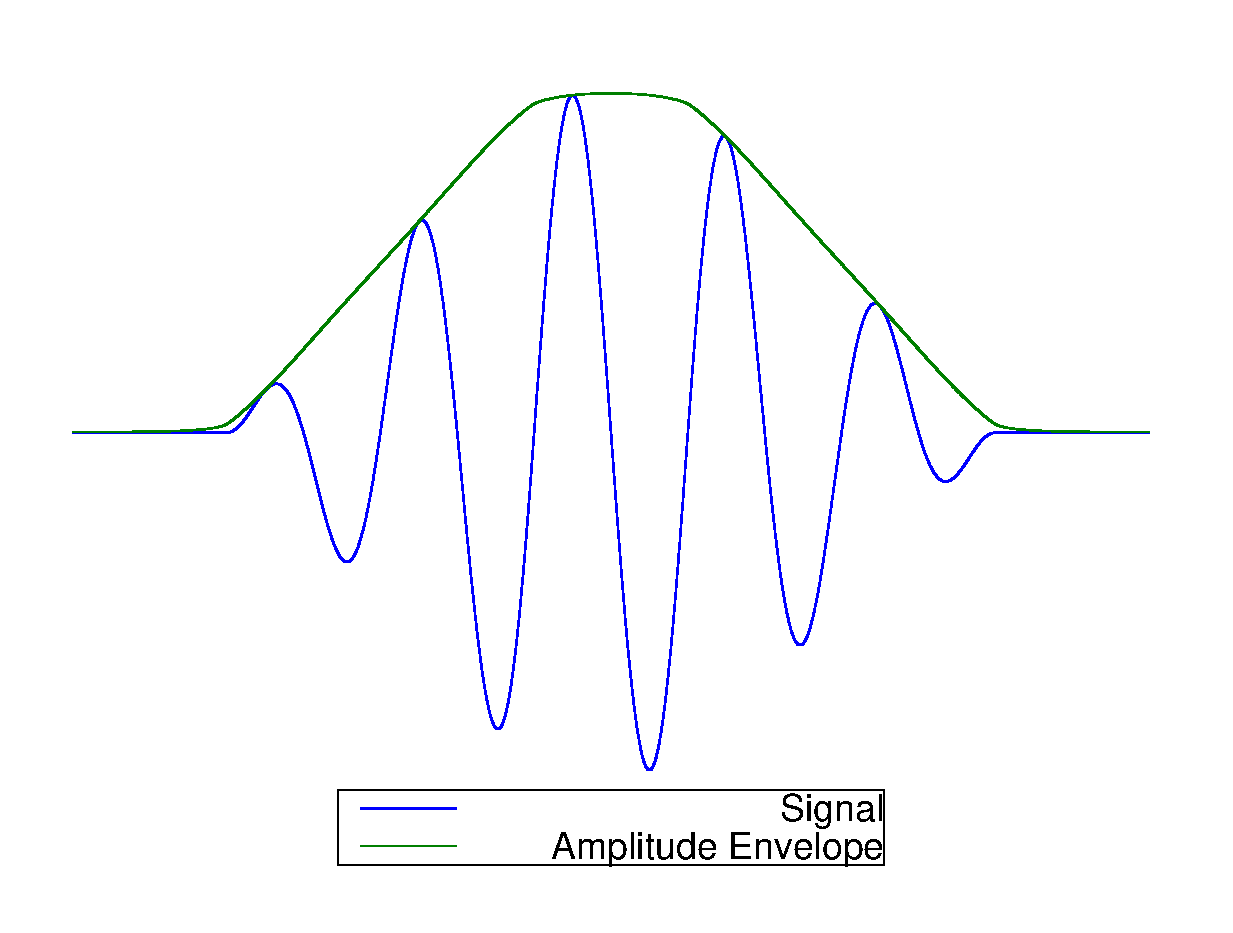
\includegraphics[width=0.6\textwidth]{chapter2/Images/AmplitudeEnvelope.eps}
			\caption{The Amplitude Envelope of a Signal.}
			\label{fig:AmplitudeEnvelope}
		\end{figure}

		Various envelope detection methods are reviewed by \citet{chang2007a}. \citet{howard2009acoustics} separates
		the envelope of a sound into three sections. The steady state section is the middle portion in which the
		timbre of the sound only varies slightly. The onset and offset sections describe the way the sound rises
		from silence to the steady state and returns to silence after. Further refinement of the description of
		amplitude envelopes leads to the ADSR (Attack, Decay, Sustain, Release) model \citep{descrivan2012music}. An
		example ADSR envelope is shown in Figure \ref{fig:ADSR}.

		\begin{figure}[h!]
			\centering
			\includegraphics[width=0.6\textwidth]{chapter2/Images/ADSR.eps}
			\caption{An ADSR Envelope.}
			\label{fig:ADSR}
		\end{figure}

		Once the amplitude envelope of a signal has been extracted further statistics can be calculated from it such
		as log attack time and temporal centroid \citep{peeters2000instrument}.

		Some other temporal features measure the oscillation or repetition of a signal. Examples are the zeros
		crossing rate and the autocorrelation, both of which can be used in pitch / frequency estimation
		\citep{mcleod2005a}.

	\subsection{Spectral Features}
	\label{sec:Timbre-LowLevelFeatures-Spectral}
		In existing timbral research is is widely reported that features of a sounds spectrum produce the largest
		effects on timbre. Simple spectral features can be calculated as statistical measures which describe the
		shape of the spectrum. For example the spectral centroid of a signal is calculated as the mean frequency
		weighted by their magnitudes. Spectral centroid is often stated as being one of the most salient audio
		features in timbre recognition \citep{freed1990auditory, lakatos2000a}. Higher order statistical moments of
		the spectrum (standard deviation, skewness and kurtosis) can be used to further describe the distribution of
		energy in the spectrum around the centroid.

		More detailed metrics in the shape of a spectrum can be calculated in the form of Mel Frequency Cepstral
		Coefficients (MFCCs). These measurements were originally used in speech recognition systems
		\citep{davis1980comparison}. More recently they have been applied to the analysis of timbre
		\citep{depoli1997sonological}. 

		Other spectral metrics consider the harmonic structure of a signal. In order to calculate these features the
		partials (prominent frequency components) of the signal must me found. The deviation of these partials from
		perfect harmonic frequencies measures the inharmonicity of the signal. \citet{fletcher1962quality} state
		that inharmonicity of some partials is necessary for the recognition of the timbre of a piano. The noise
		energy in a signal describes any energy which is does not contribute to a partial. The noisiness is then
		measured as the ratio of the noise energy to the total energy in the signal \citep{serra1998sound}.

		Further analysis can be performed by finding the harmonic partials of the signal. In detecting the harmonic
		partials it is usual to allow for a slight deviation from perfect harmonic structure, as described by
		\citet{peeters2011the}. Several metrics have been suggested which constitute the ratio of energy between two
		different sets of harmonic partials. The tristimulus metrics proposed by \citet{pollard1982a} split the
		harmonic series in to three sections, the fundamental frequency, the second through fourth harmonics and,
		the rest of the higher order harmonics. Ratios between each of these sections and the total energy in the
		harmonics are calculated. Another commonly used metric is the ratio between energy in the odd and even order
		harmonic partials. This was found to be a salient feature in the judgement of timbre dissimilarity by
		\citet{hall2010importance}. 

		\note
		{
			Spectro-temporal features exist such as spectral flux.
		}


\section{Psychoacoustic Principles}
\label{sec:Timbre-PsychoacousticPrinciples}
	Psychoacoustics is a field which deals with the perception of sound. The existing literature concerns the study of
	the human hearing system and how it responds to certain aspects of audio stimuli. Several different areas of audio
	perception have been researched. Methods have been devised to model the human perception of loudness
	\citep{moore1997a} and pitch \citep{gerhard2003pitch}. Other research considers the human hearing systems ability to
	locate sound sources \citep{blauert1997spatial}. 

	As discussed in Section \ref{sec:Timbre-LowLevelFeatures-Spectral} there are several metrics to describe the
	spectral content of a signal. While it may be possible to measure changes in values of these features, the changes
	may not be detectable by the human hearing system. Psychoacoustic models allow us to determine how audio signals are
	interpreted by the human hearing system and how well we will notice such changes.

	\subsection{Critical Bands}
	\label{sec:Timbre-PsychoacousticPrinciples-CriticalBands}
		The part of the inner ear which deals with frequency separation is know as the basilar membrane. This is a
		structure which resonates at different frequencies along its length. Low frequencies at one end to high at
		the other. A sinusoidal tone excites a portion of the basilar membrane corresponding to a narrow band of
		frequencies. Two tones whose excitation bands overlap will interfere with how each other are perceived by
		the listener.

		The basilar membrane can be modelled as a filter bank comprised of band pass filters. Each of these
		auditory filters represents the region of the membrane excited by a sinusoidal tone at its centre
		frequency. The bandwidth of these filters is known as the critical bandwidth. Portions of signals will
		interfere with the perception of others which are within one critical bandwidth.
		\citet{glasberg1990derivation} simplify the auditory filters by modelling them as rectangular filters. The
		bandwidth of these filters known as the equivalent rectangular bandwidth (ERB) and can be approximated using
		Equation \ref{eq:ERB}.

		\begin{equation}
			ERB(f_{c}) = 24.7(4.37f_{c} + 1)
			\label{eq:ERB}
		\end{equation}

		Where $f_{c}$ is the center frequency of the auditory filter in kHz and $ERB(f_{c})$ is the equivalent
		rectangular bandwidth, in Hz, at that frequency.

		\citet{howard2009acoustics} discusses the perception of two tones, sounded simultaneously, as they get
		further apart in frequency. When within 15Hz of one another the two tones are perceived as a single sound
		with a sinusoidally varying amplitude. The frequency of this variation is equal to the difference in
		frequency of the tones. As the difference in frequencies gets greater then 15Hz this amplitude modulation
		becomes fast enough for it to be perceived as a roughness in texture rather than `beats' in the amplitude.
		In between 15Hz and the critical bandwidth the perceived sound transitions from a single sound to two
		separate sounds but still with a rough texture. Once the difference in frequencies exceeds the critical
		bandwidth the two tones are perceived as separate smooth tones. These effects are summarised in Figure
		\ref{fig:ToneSeparation}.

		\begin{figure}[h!]
			\centering
			\begin{tikzpicture}

				\draw [thick, ->] (0, 0) -- (10, 0);
				\draw (0, 1) -- (10, 1);
				\draw (0, 0) -- (0, 2) -- (10, 2);

				\draw (0, 0) -- (0, -2pt) node [anchor=north] {0};
				\draw (2, 0) -- (2, -2pt) node [anchor=north] {15};
				\draw (8, 0) -- (8, -2pt) node [anchor=north] {CB};

				\fill [pattern=north west lines] (1.75, 0) rectangle (2.25, 1);
				\fill [pattern=north west lines] (7.75, 0) rectangle (8.25, 1);
				\fill [pattern=north west lines] (5.75, 1) rectangle (6.25, 2);

				\node at (0.875, 0.5) {Beats};
				\node at (5, 0.5) {Rough};
				\node at (9.125, 0.5) {Smooth};
				\node at (2.875, 1.5) {Fused};
				\node at (8.125, 1.5) {Separate};

				\node at (5, -1) {Frequency Difference (Hz)};

			\end{tikzpicture}
			\caption{The perceived of two tones as they move further apart in frequency. Hashed areas represent
				 the transition between perceived effects. CB denotes the critical bandwidth.}
			\label{fig:ToneSeparation}
		\end{figure}

		It is evident from Equation \ref{eq:ERB} that the critical bandwidth increases with frequency. This together
		with the perceptual information shown in Figure \ref{fig:ToneSeparation} suggests that tones separated by
		the same amount will be heard as separate if they or both low in frequency but as their frequencies rise
		they will start to be perceived as a single fused sound.

	\subsection{Specific Loudness}
	\label{sec:Timbre-PsychoacousticPrinciples-SpecificLoudness}
		In hearing models for measuring loudness it is common to split the audible spectrum into bands which all
		have the same perceived width. Before calculating the total loudness the specific loudness for each of these
		bands is calculated. The procedure for doing this is beyond the scope of this report. A description of this
		process is provided by \citet{moore1997a}. The specific loudness measures the perceived loudness of a signal
		in a given frequency range. For the analysis of the perception of timbre this allows for better modelling of
		what portions of a signals spectrum are audible. While the spectrum describes what frequency content is
		present in the signal, the specific loudness describes how much of each frequency is perceived by a
		listener.

		A widely used set of bands was proposed by \citet{zwicker1961subdivision} who spilt the spectrum into 24
		bands, each one critical bandwidth wide. These bands are known and the bark bands and provide a perceptual
		unit of frequency, the bark. Integer values of barks occur at the boundaries between two bark bands. An
		change in frequency of one bark is equal to one critical bandwidth.

	\note
	{
		Perhaps some more on masking. Although it may be wasted space.
	}

\section{Timbral Features}
\label{sec:Timbre-TimbralFeatures}
	Models have been developed in the literature to describe certain aspects of the timbre of a sound. Two such models
	are those for describing auditory sharpness and roughness.
	
	\subsection{Sharpness}
		\citet{fastl2007psychoacoustics} discuss the factors leading to the perception of sharpness. The sharpness
		of a signal depends on the ratio of high and low frequency content. Increasing the amount of high frequency
		content increases the sharpness of a signal. The sharpness can also be reduced by adding more low frequency
		content to a signal. They produce a metric from this information for the measurement of perceived sharpness.
		The sharpness is calculated using Equation \ref{eq:Sharpness}.

		\begin{equation}
			S = 0.11\frac{\int_{0}^{24Bark} N'g(z)zdz}{\int_{0}^{24Bark}N'dz}
			\label{eq:Sharpness}
		\end{equation}

		Where $S$ is the sharpness, $N'$ is the specific loudness, $z$ is frequency in barks and $g(z)$ is a
		weighting function designed to emphasises the presence of high frequency content.

		\citet{marui2006predicting} run listening experiments to test how well perceived sharpness can be predicted
		using this metric. They find that it does not predict the sharpness of broadband noise accurately and
		propose an improved metric which is the product of the value from Equation \ref{eq:Sharpness} and the
		spectral variance of the specific loudness.

	\subsection{Roughness}
	A sensation of roughness was discussed in Section \ref{sec:Timbre-PsychoacousticPrinciples-CriticalBands}. Here the
	roughness was due to the rapid amplitude modulation produces as a result of summing two sinusoids which are close in
	frequency. 

	\note
	{
		\citet{fastl2007psychoacoustics} and \citet{vassilakis2010psychoacoustic} both talk about the contribution
		of amplitude modulation to roughness.
	}

\section{Parameterisation of Timbre}
\label{sec:Timbre-Parameterisation}
	\note{Analysis of timbre spaces and discussion on salience of some features as given in the literature.}

	\subsection{Dissimilarity Tests}
	\label{sec:Timbre-Dissimilarity}
		\note
		{
			A more traditional approach, \citet{grey1977multidimensional} and all the copycat lot 
			\citep{burgoyne2008a, caclin2005acoustic}.
		}

	\subsection{VAME}
	\label{sec:Timbre-VAME}
		\note{\citet{kendall1993verbal1, kendall1993verbal2} trying to upset the status quo.}

	\subsection{Parameter Space}
	\label{sec:Timbre-ParameterSpaces}
	\note{Research like Social EQ and stuff \citep{cartwright2013socialeq, seetharaman2014crowdsourcing}.}

\section{Controlling Timbre}
\label{sec:Timbre-Control}
	\note{Lots of them synthesis dudes have tried to control the beast. \citet{zacharakis2011an} did some stuff.}
	
	\note
	{
		Some dudes do morphing (analysis resynthesis from what I remember) like good old 
		\citet{williams2007perceptually, williams2009perceptually, williams2010perceptually}
	}

%Review of existing harmonic excitation.
%	Nonlinear Systems
%		Traditional Metrics (THD, IMD)
%		Minimisation of Nonlinear Distortion
%		Advent of "Nonlinear Niceness"
%	Timbre of nonlinear distortions (Martens and Marui type shit)
%	Uses of Harmonic Excitation
%	Harmonic Generation Methods
%		Static Nonlinearities
%		Bandwidth Extension (high frequency reconstruction)
%		Individual Harmonic Generation (SMC paper)
%		Psychoacoustic Enhancers

\chapter{Harmonic Excitation}
\label{chap:Excitation}

\section{Introduction}
\label{sec:Excitation-Introduction}
	Nonlinear distortion is an inherent part of an analogue signal path. It alters the dynamic variation of signals and
	introduces new spectral components. Its use as a creative effect is best know by guitar players
	\citep{dutilleux2011nonlinear}. This was due to the use of values in early guitar amplifiers imparting nonlinear
	transforms onto the audio signal. This distorted sound became desirable and several electronic circuits were
	developed with the purpose of inducing nonlinear distortion. More recently research into modelling these distortion
	circuits in the digital domain has been carried out, such as that done by \citet{pakarinen2009a}. Several
	researchers have also worked on creating novel digital distortion techniques \citep{fernandez-cid2001distortion,
	pekonen2008coefficient, puckette2007patch}.

	Distortion is a very broad term which is typically used to describe unwanted effects. For this work a better
	defined term, harmonic excitation, will be used to refer to the deliberate and controlled application of nonlinear
	systems in order to introduce new frequency components to a signal. \citet{dutilleux2011nonlinear} defines
	excitation as the process of controlling timbre through the emphasis of certain frequencies. While this is possible
	with linear systems, such as equalisers, nonlinear systems provide more flexibility as they can add energy in areas
	of the spectrum where the original signal had none.

	This chapter will review how nonlinear systems have been analysed in previous audio research, how their effects are
	quantified and the timbral transformations they impart. The current uses of harmonic excitation in audio
	engineering are then discussed in Section \ref{sec:Excitation-Uses}. A list of criteria with which to evaluate
	harmonic excitation methods for use in real time timbral control is developed in Section
	\ref{sec:Excitation-Evaluation}.  Section \ref{sec:Excitation-Methods} then describes several methods for harmonic
	excitation and how they perform in these areas.  Issues with certain methods are identified and ways to overcome
	them suggested.

\section{Analysis of Nonlinear Systems}
\label{sec:Excitation-AnalysisOfNonlinearSystems}
	\note 
	{
		What is a nonlinear system?
	}

	The analysis of nonlinear system is more complicated that that of linear systems. This is due to more features of
	the input signal affecting how the system responds. In the field of audio engineering much of the literature
	concerning nonlinearities has to do with minimising distortion or measuring the maximum allowable levels of
	distortion. Several distortion metrics have been developed each with there own uses. A review of many of these
	metrics is given by \cite{voishvillo2006assessment}, some of which will be discussed in this section.

	\subsection{Objective Distortion Metrics}
	\label{sec:Excitation-Analysis-Metrics}
		Total Harmonic Distortion (THD) and Intermodulation Distortion (IMD) are the traditional objective measures
		of distortion \citep{czerwinski2001multitone1}. THD measures the level of new frequency components
		introduced by a system which are harmonically related to the original signal.  There are two different ways
		in which THD is calculated. These have been denoted $THD_{F}$ and $THD_{R}$ by \citet{shmilovitz2005on} and
		are calculated using Equations \ref{eq:thdf} and \ref{eq:thdr} respectively.

		\begin{equation}
			THD_{F} = \frac{\sqrt{\sum_{n = 2}^{\infty} A_{n}^{2}}}{A_{1}}
			\label{eq:thdf}
		\end{equation}

		\begin{equation}
			THD_{R} = \sqrt{\frac{\sum_{n = 2}^{\infty} A_{n}^{2}}{\sum_{n = 1}^{\infty} A_{n}^{2}}}
			\label{eq:thdr}
		\end{equation}

		Where $A_n$ is the amplitude of the $n_{th}$ harmonic. 

		Both these methods been used in recent work published in the audio field ($THD_{F}$ by
		\citet{fleischmann2014a} and $THD_{R}$ by \citet{dutilleux2011nonlinear}). The lack of standardisation for
		this metric makes it difficult to compare experiment results reported by different sources.

		IMD is a measure of the new spectral content introduced by a system as a result of intermodulation between
		the frequency components of the original signal. There are several different standards for the calculation
		of IMD some of which are listed by \citet{voishvillo2006assessment}.

		THD and IMD give very limited information about the response of nonlinear systems. They are typically
		measured using simple input signals which are not representative of the signals a system would process in
		actual use. Given that nonlinear systems my not satisfy the condition of superposition a system may process
		simple and complex signals in vastly differing manners. 

		These metrics also give no indication of the perceived degradation in audio quality a system introduces. A
		signal with a high THD values may sound less distorted that one with a small THD. Several researchers have
		developed new distortion metrics which indicate the perceived amount of distortion.

		\citet{geddes2003auditory} suggest some psychoacoustic principles which may be applicable to the analysis
		of nonlinear distortion:

		\begin{itemize}
			\item New frequency components introduced, with lower frequencies that the original components,
				will be more perceptible.
			\item Higher order nonlinearity artefacts will be more perceptible.
			\item Nonlinearities which affect lower amplitude signals will be more perceptible.
		\end{itemize}

		\citet{voishvillo2006assessment} adds that the perception of distortion is decreased at the very high and
		low ends of the frequency spectrum.

		The GedLee metric, proposed by \citet{geddes2003auditory}, measures how much a nonlinearity will be
		perceived through analysis of its characteristic curve. It is calculated using Equation \ref{eq:gedlee}.

		\begin{equation}
			G_{m} = \sqrt{\int_{-1}^{1} \left( \cos \left( \frac{x\pi}{2} \right) \right)^{2}
				      \left( \frac{d^{2}}{dx^{2}} T(x) \right)^{2} dx}
			\label{eq:gedlee}
		\end{equation}

		Where $T(x)$ is the characteristic curve of the nonlinearity in question.

		A considerable advantage of the GedLee metric is that it directly measures the system in question rather
		than signals processed by it. This should allow measurements taken using the metric to describe the audible
		degradation of any signal processed by a system. \citet{lee2003auditory} provide results of an experiment
		in which their metric was tested against THD and IMD as a rating of audio quality. They show that for low
		levels of distortion the GedLee metric correlates with subjective audio quality ratings. THD and IMD are
		both found to not correlate well with perceived quality.

		In Equation \ref{eq:gedlee} the system being analysed is assumed to be a simple static nonlinearity. Many
		nonlinear systems are more complex than this and may exhibit frequency dependant or time varying behaviour.
		While the GedLee metric may provide a good, signal independent, measure of distortion, it is only
		applicable to a subset of nonlinear systems.

		\citet{tan2003the} also developed a perceptual metric for distortion, Distortion Score (DS), which they
		then improved upon to create the R\sub{nonlin} metric \citep{tan2004predicting}. Both these metrics rely on
		analysing signals which have been processed so they may not give results which can be applied as generally
		as those using the GedLee metric. Where these metrics have an advantage is that they use models of the
		human hearing system to better approximate the perceived level of distortion.

		To calculate the DS the audio is split into frequency bands which model the auditory filters of the
		cochlear. These auditory filters represent bands in which two tones will interfere with the perception of
		each other \citep{fastl2007psychoacoustics}. Tones can be masked (made inaudible) by other tones within the
		same auditory filter band. By processing the audio in this manner the DS metric can take account of
		elements of the distortion which may not be perceptible because of masking.
		
		The R\sub{nonlin} metric improves on this model of the hearing system by including a filter with a
		frequency response similar to that of the outer and middle ear. The filter used is as described by
		\citet{glasberg2002a}, it attenuates frequencies at either end of the audible spectrum. This models the
		decreased perception of distortion at these frequencies discussed earlier.

		\citet{tan2004predicting} report greater correlation between R\sub{nonlin} and perceived audio quality then
		\citet{lee2003auditory} do for the GedLee metric. They also demonstrate how accurate the R\sub{nonlin}
		metric is in predicting the perceived distortion level introduced to music and speech signals.

		The research discussed in this section has focused on measuring the extent to which unwanted distortion can
		be perceived. This does not provide enough information for the description of timbre. The listening test
		performed to verify the developed metrics asked subjects to rate the quality of audio samples. Nonlinear
		distortion could alter the timbre of audio without deteriorating its perceived quality. It may also be
		possible to describe the timbre of different nonlinear distortions further rather than ranking them on the
		same distortion scale. Research has been carried out into the timbre of distortion as discussed in Section
		\ref{sec:Excitation-Timbre}.

		\subsection{Nonlinear Modelling}
		Various techniques for modelling nonlinear systems have been developed in the mathematics and engineering
		literature. These models allow for more in depth analysis of a system as well as replicating its effects in
		the digital domain. Summaries of some of these modelling techniques can be found in the work by
		\citet{janczak2005identification} and \citet{ogunfunmi2007adaptive}.

		Two nonlinear modelling techniques have found use in audio processing:

		\begin{itemize}
			\item Wave Digital Filters as discussed by \citet{fettweis1986wave}.
			\item The Synchronised Swept Sine Method as described by \citet{novak2010nonlinear}.
		\end{itemize}

		These techniques are summarised here.

		\subsubsection{Wave Digital Filters}
			Wave digital filters are a class of filter which can be used to emulate analogue circuits. The
			process of creating a digital of a circuit involves constructing a `tree' of blocks. These blocks
			represent either electronic components, or connections between components in a circuit. Each block
			obeys a certain set of rules when presented with a signal. Blocks have been developed for modelling
			nonlinear circuit elements such as operational amplifiers and diodes \citep{paiva2012emulation}.

			While wave digital filters can accurately represent a nonlinear system there are some disadvantages.
			As systems get more complex traversing the `tree' of blocks in order to calculate the output signal
			takes more computation. This presents problems when real time system response is needed. There are
			also certain circuit topologies which cannot be represented in the wave digital domain
			\citep{valimaki2011virtual}. Another consideration is that knowledge of the circuitry inside a
			system being modelled is needed. This might not always be available.

		\subsubsection{The Synchronised Swept Sine Method}
			The synchronised swept sine method is a technique for identifying nonlinear systems without prior
			knowledge of their operation. The details of its operation are describe by
			\citet{novak2010nonlinear}. The result of the testing is a series of filter kernels to be used in
			the model shown in Figure \ref{fig:hammerstein}.

			\begin{figure}[h!]
				\centering
				\begin{tikzpicture}
					\node (Sig2) [draw] at (1, 3) {$x[n]^{2}$};
					\node (Sig3) [draw] at (1, 2) {$x[n]^{3}$};
					\node (SigN) [draw] at (1, 0.5) {$x[n]^{N}$};

					\node (Filter1) [draw] at (3, 4) {$A_{1}(f)$};
					\node (Filter2) [draw] at (3, 3) {$A_{2}(f)$};
					\node (Filter3) [draw] at (3, 2) {$A_{3}(f)$};
					\node (FilterN) [draw] at (3, 0.5) {$A_{N}(f)$};

					\draw (Sig2) -- (Filter2);
					\draw (Sig3) -- (Filter3);
					\draw (SigN) -- (FilterN);

					\draw [dots] (Sig3) -- (SigN);
					\draw [dots] (Filter3) -- (FilterN);

					\coordinate (Out1) at (4.5, 4);
					\coordinate (Out2) at (4.5, 3);
					\coordinate (Out3) at (4.5, 2);
					\coordinate (OutN) at (4.5, 0.5);

					\draw (Filter1) -- (Out1);
					\draw (Filter2) -- (Out2);
					\draw (Filter3) -- (Out3);
					\draw (FilterN) -- (OutN);

					\node (Add) [operator] at (5, 2.25) {+};
					\draw (Out1) -- (Add);
					\draw (Out2) -- (Add);
					\draw (Out3) -- (Add);
					\draw (OutN) -- (Add);

					\coordinate (In1) at (-0.5, 4);
					\coordinate (In2) at (-0.5, 3);
					\coordinate (In3) at (-0.5, 2);
					\coordinate (InN) at (-0.5, 0.5);

					\draw (In1) -- (Filter1);
					\draw (In2) -- (Sig2);
					\draw (In3) -- (Sig3);
					\draw (InN) -- (SigN);
					\draw (InN) -- (In1);

					\node (In) at (-1.25, 2.25) {$x[n]$};
					\coordinate (InMid) at (-0.5, 2.25);
					\draw (In) -- (InMid);

					\node (Out) at (6, 2.25) {$y[n]$};
					\draw (Add) -- (Out);

				\end{tikzpicture}
				\caption{Generalised Polynomial Hammerstein Model.}
				\label{fig:hammerstein}
			\end{figure}

			The model is, in effect, an extension of a Taylor Series of order $N$. The input is raised to each
			individual power, 1 through $N$, and each of these signals is filtered by an individual kernel,
			$A_{N}(f)$. The resultant signals are then summed to produce the output.

			This method is easier to implement that a wave digital filter as no prior knowledge of the system is
			needed. The amount of computation time needed to process a signal is also considerably less. There
			are however some disadvantages. There is no account for the dependence of the system on the
			amplitude of the input signal. This is shown by \citet{novak2010analysis} who demonstrate how two
			different circuits are emulated with different degrees of accuracy. The is also no definite way of
			deciding what order Hammerstein model to use prior to testing.

\section{Timbre of Nonlinear Distortion}
\label{sec:Excitation-Timbre}
	There is a wealth of research into how low level audio features influence timbre \note{(probably refer to stuff in
	the timbre chapter here)}. The mappings between low level features and semantic features from the literature can be
	applied to harmonic excitation effects provided the excitation method used can influence the required low level
	features. There may be semantic terms used to describe the timbre of nonlinear distortion which are seldom used to
	describe other timbres. The majority of timbral research does not focus on nonlinear distortion and as such does not
	highlight these semantic terms. There have been some publications specifically discussing the timbral effects of
	nonlinear distortion. Their findings are discussed in this section.

	\citet{marui2005predicting} suggest that one of the primary outcomes of nonlinear distortion is the moving
	of spectral energy between low and high frequencies. An effect they propose correlates with the descriptors
	sharpness and brightness. In order to discover other timbral properties of nonlinear distortion they performed
	listening tests in which distorted guitar samples were assessed. The samples were each processed with different
	nonlinear systems and then further processed so that they had matching Zwicker Sharpnesses (an objective measure of
	sharpness \cite{fastl2007psychoacoustics}). This sharpness matching was does so that difference in timbre not
	related to sharpness could be more easily observed. During the listening tests subjects were asked to rate the
	dissimilarity of samples presented in pairs. They were also asked to grade each individual sample on the bipolar
	adjective scales shown in Table \ref{tab:distortionDescriptors}.

	\begin{table}[h!]
		\centering
		\begin{tabular}{|c|C{3cm}cC{3cm}|}
			\hline
			\bf{No.} & \multicolumn{3}{|c|}{\bf{Adjectives}} \tabularnewline
			\hline
			\hline
			1 & dark & $\Longleftrightarrow$ & bright \tabularnewline
			\hline
			2 & rough & $\Longleftrightarrow$ & smooth \tabularnewline
			\hline
			3 & diffuse & $\Longleftrightarrow$ & compact \tabularnewline
			\hline
			4 & thin & $\Longleftrightarrow$ & thick \tabularnewline
			\hline
			5 & sharp & $\Longleftrightarrow$ & dull \tabularnewline
			\hline
			6 & light & $\Longleftrightarrow$ & heavy \tabularnewline
			\hline
			7 & hard & $\Longleftrightarrow$ & soft \tabularnewline
			\hline
			8 & clear & $\Longleftrightarrow$ & muddy \tabularnewline
			\hline
			9 & clamorous & $\Longleftrightarrow$ & calm \tabularnewline
			\hline
			10 & string & $\Longleftrightarrow$ & weak \tabularnewline
			\hline
			11 & uncomfortably loud & $\Longleftrightarrow$ & comfortable \tabularnewline
			\hline
		\end{tabular}
		\caption{Bipolar adjectives scales used by \citet{marui2005predicting} to assess the perception of
		         distortion.}
		\label{tab:distortionDescriptors}
	\end{table}

	Their results suggest that the differences between different nonlinearities can be described by `thickness' and, to
	a lesser extent, `diffuseness'. These results are also met by a second experiment in which a triadic comparison
	method is used to assess the dissimilarities between samples \citep{marui2005constructing}.

	Both these experiments were conducted in Japanese and the descriptors were translated to English for publication.
	The descriptors were initially chosen during an experiment by \citet{martens2002relating}. From this experiment it
	was shown that speakers of Japanese and speakers of Sinhalese disagree on the how these terms are used to describe
	timbre. It is expected that there will be similar differences in presenting the descriptors to English speakers.

	\note
	{
		Resolving harmonics in the cochlea. Low order harmonics are generally resolved individually so their
		individual levels will have a strong effect on perceived timbre. Higher order harmonics are resolved in
		groups so less manipulation is needed \citep{howard2009acoustics}.
	}

	\note
	{
		More recent papers \citep{wilson2014characterisation, tsumoto2015investigating}.
	}

	\note
	{
		Smooth this transition here. Uses of nonlinear systems, highlighting focus on excitation for timbral
		control.
	}

\section{Uses of Harmonic Excitation}
\label{sec:Excitation-Uses}
	Harmonic excitation is used for several tasks in audio engineering:

	\note
	{
		Perhaps not bullet points. That implies equal emphasis.
	}

	\begin{itemize}
		\item As a creative audio effect used to manipulate the timbre of sounds for music production.
		\item To reconstruct high frequency information in perceptual audio compression codecs.
		\item To extend the perceived bandwidth of loudspeakers.
		\item To enhance the intelligibility of speech. 
	\end{itemize}

	\subsection{High Frequency Reconstruction}
	\label{sec:Excitation-Uses-Reconstruction}
		In digital systems it can be beneficial to reduce the amount of data needed to represent an audio signal.
		This is done either to reduce the storage space needed or reduce the data rate required to transmit a
		signal. As a higher data rate is needed to represent high frequencies these frequencies are removed during
		the compression process. A lot of research has been carried out to develop methods by which these high
		frequencies can be estimated during the decoding process. This allows for the bandwidth to be constricted
		for storage or transmission but the full bandwidth to be restored when required.

		When using audio codecs the original signal, along with is high frequency components, is available before
		compression is applied. This means that some parameters relating to the high frequency content can be
		recorded and used to aid in the reconstruction of the high frequencies later \citep{dietz2002spectral,
		friedrich2007spectral}. The high frequency content is estimated from the low frequency information and
		then further shaped using these parameters. This leads to a distinction between `blind' and `non blind'
		methods for reconstructing the high frequencies. A `blind' method uses only the information present in the
		low frequency signal, whereas `non blind' methods make use of recorded parameters to increase the accuracy
		of the reconstruction.

		In the literature several different methods for reconstruction of the higher frequencies are suggested:

		\begin{itemize}
			\item Through the use of a nonlinear device \citep{larsen2002efficient, sha2010high}.
			\item Spectral replication as done by \citet{nagel2010a}. This essential frequency shift the
			      spectrum into a higher band.
			\item Spectral folding as used by \citet{friedrich2007spectral}. This creates a mirror image of the
			      existing spectrum around the highest frequency.
			\item Spectral stretching a used by \citet{nagel2009a}. This stretches the existing spectrum to the
		              desired bandwidth.
		\end{itemize}

		These methods could be utilised in creative audio effects. They all introduce new harmonic spectral
		components which may enhance perceptual attributes of a sound. In this situation there is not any
		information about how the higher harmonics might behave so the system will have to operate `blindly'. It is
		worth considering that when using these methods as an audio effect the objective is not to try and
		replicate high frequency content which is missing. The generation of new, high order, harmonics does not
		require the same degree of accuracy. The accuracy lost through using `blind' bandwidth extension methods is
		not a great concern for creative timbral manipulation work.

		Information on how these methods can be implemented as simple harmonic exciters is given in Section
		\ref{sec:Excitation-Methods}.

	\subsection{Perceptual Low Frequency Reinforcement}
	\label{sec:Excitation-Uses-Reinforcement}
		Small loudspeakers are incapable of reproducing low frequency signals at sufficient amplitudes. Harmonic
		excitation can be used to psychoacoustically extend the bandwidth of loudspeakers into the lower end of the
		spectrum. Harmonic content is added to the signal in order to evoke the perception of lower pitch sounds.

		The pitch of harmonically structured sounds is the same as that of it's fundamental frequency. No energy
		need be present at the fundamental for its pitch to be perceived however. So long as a sufficient
		proportion of the harmonic structure remains the original pitch can still be perceived. This phenomenon is
		commonly referred to as the missing fundamental \citep{plack2005the}.

		This technique is implemented in effects such as Waves' MaxxBass \citep{ben-tzur1999the}. Implementation
		techniques have been discussed by \citet{larsen2002reproducing} and \citet{gan2001virtual}.

	\subsection{Audio Enhancement}
	\label{sec:Excitation-Uses-Enhancement}
		One of the most commonly used enhancement effects is the Aphex Aural Exciter.  \citet{shekar2013modeling}
		states that this effect enhances brightness and clarity of a sound through the application of nonlinear
		distortion.

		\citet{chalupper2000aural} ran several tests to determine the effects the Aural Exciter has on different
		audio samples, concluding that it operates as a `sharpness' maximiser. The analysis of the device is very
		basic, comprising of a frequency response and an analysis of the spectral alterations made to a 2kHz sine
		wave. The frequency response shows the liner processing undertaken by the device, showing that it amplifies
		high frequency content. The sine wave response analysis is used to demonstrate the nonlinear elements of
		the device. 

		\citet{dutilleux2011nonlinear} provides a slightly more in depth analysis of the Aural Exciter showing the
		spectral alterations make to a chirp signal. This gives information about how the nonlinear section of the
		device responds to different input frequencies. It is seen that a hight level of second harmonic distortion
		is produced. It is not mentioned however, what the exciter's parameters were set to during these tests. For
		this reason it is difficult to compare these results with those collected by \citet{chalupper2000aural}
		which see to disagree as they show a larger amount of new spectral content being introduced. Neither work
		accounts for differences in processing depending on the input amplitude.

\section{Evaluation Criteria for Harmonic Excitation Methods} % section name not very clear
\label{sec:Excitation-Evaluation}
	\note
	{
		Specify that we are only dealing with the use of exciters for perceptual control.
	}
	
	There are many different classes of nonlinear system which are used in audio processing. Each of these has its own
	characteristics. There are several properties to look at when evaluating a nonlinear system for use in real time
	timbral control. These are:

	\begin{itemize}
		\item Low Complexity.
		\item Homogeneity
		\item Spectral Characteristics.
		\item Temporal Characteristics.
		\item Flexibility.
%		\item Naturalness.
	\end{itemize}

	The following sections will discuss what behaviour is desirable in these areas.

	\subsection{Complexity}
	\label{sec:Excitation-Evaluation-Complexity}
		Audio effects are typically required to operate in real time. This speeds up music production as effect
		parameters can be adjusted while audio is playing and the results heard immediately. In order to achieve
		this, effects must process audio with minimal latency. 

		In order to ease the computational load on the processor, audio processing if often done in blocks. A
		certain number of samples are recorded into a buffer and then all processed at once. This introduces some
		latency into the system, one buffers worth of samples must be collected from the input before an output can
		be produced. The larger the processing buffer size the more latency but the less the computational load. Any
		processing applied to the block of audio must be completed within the allowed latency time. If not there
		will be gaps between blocks during playback causing audible anomalies.

		For real time audio effects it is crucial to keep throughput latency to a minimum. \citet{lester2007the}
		suggest that, depending on the scenario, latencies as small as 1.4ms could be deemed unacceptable. In order
		to keep latency to a minimum, processing algorithms should be able to run in real time when using a small
		buffer size.

	\subsection{Homogeneity}
	\label{sec:Excitation-Evaluation-Homogeneity}
		In order to aid in the intuitiveness of an audio effect it should produce a similar perceptual effect
		across a wide range of input signals. This is not the case with traditional audio signal processing
		methods. Take the EQ for example. We can set up an EQ to boost some frequencies in a desired range. A
		problem arises where we process signals which have no energy in this frequency range. For some signals
		there will be a noticeable change in the spectral characteristics, but other signals will remain unchanged.

		This problem is compounded when the effect being applied is non-homogeneous. A homogeneous system is one
		whose behaviour does not depend on the input amplitude of the input. Where $f$ is a homogeneous system we
		have:

		\[ f(ax) = af(x) \]

		Where $a$ is some scaling factor of the input $x$.
		
		Nonlinear systems are typically non-homogeneous. This is undesirable when using them to achieve timbral
		control as it means the effects are less easy to predict. Different timbral transformations could be
		applied to the same signal if its amplitude is changed slightly. From a user point of view this makes
		control of the system less intuitive as control parameters can change function depending on signal level.

		\note{Mention of homogeneous nonlinear systems \citep{larsen2004audio}.}

		There do exist homogeneous nonlinear systems. These are a minority however and lack some of the desirable
		features that some non-homogeneous systems have. In some cases steps can be taken to make non-homogeneous
		systems homogeneous. These will be discussed where appropriate in Section \ref{sec:Excitation-Methods}

	\subsection{Spectral Characteristics}
	\label{sec:Excitation-Evaluation-SpectralCharacteristics}
		All the systems discussed in this chapter introduce new spectral content to a signal. For timbral control
		it is desirable to have precise control over which frequencies are introduced. Some algorithms introduce
		large bands of frequencies whereas others can be used to excite single harmonics. 
		
		This content can be ascribed to three different groups:

		\begin{itemize}
			\item Harmonic Distortion
			\item Intermodulation Distortion
			\item Aliasing
		\end{itemize}

		These groups are all produced via different mechanisms. 

		\subsubsection*{Harmonic Distortion}
			Harmonic distortion typically refers to the harmonic frequency content generated when a sinusoidal
			signal undergoes nonlinear processing. These are equivalent to the cross modulation components
			introduced by modulating the signal with itself. This mechanism also operates on more complex
			signals. Each individual frequency component being modulated by itself and generating its own set
			of harmonics.

			The spectral effects of harmonic distortion are easy to predict. The response of a system to a
			sinusoidal input can be measured. Then, taking into account any frequency dependence the system may
			have, a general model of how the system will respond to a sinusoid of any frequency can be
			constructed.

		\subsubsection*{Intermodulation Distortion}
			Intermodulation distortion occurs when signals with two or more frequency components undergo
			nonlinear processing. New frequency components are generated equivalent to the cross modulation
			components of each combination of frequency components modulating each other. The more complex the
			spectrum of a signal the more intermodulation components will be introduced. Unlike with harmonic
			distortion it is difficult to generalise the intermodulation components produced by a system. 

		\subsubsection*{Aliasing}
			Aliasing arises due to the discrete nature of digital audio signals. The sampling frequency of a
			discrete signal imposes a restriction on the highest frequency which can be represented. This
			frequency is known as the Nyquist frequency ($f_{N}$) and can be calculated using Equation
			\ref{eq:nyquist}.

			\begin{equation}
				f_{N} = \frac{f_{s}}{2}
				\label{eq:nyquist}
			\end{equation}

			Where $f_{s}$ is the sampling rate of the signal.

			When sampling a signal frequency content above the Nyquist is represented as alias frequencies
			within the bandwidth allowed by the sampling frequency. The alias frequency can be calculated using
			Equation \ref{eq:aliasing}.

			\begin{equation}
				f_{alias} = |f - Nf_{s}|
				\label{eq:aliasing}
			\end{equation}

			Where $f$ is the original frequency and $Nf_{s}$ is the integer multiple of the sampling
			frequency closest to it.

			The new frequency content introduced to a discrete signal via nonlinear processing is also subject
			to aliasing. This can cause problems in the uniformity of behaviour of a system in different
			scenarios as the spectral content introduced will depend on the sampling frequency of the signal
			being processed. Thus the perceived timbral transformation may also depend on the sampling
			frequency.

			\citep{vetter2013estimation} upsample signals by a factor of 32 prior to applying
			the nonlinearity. Afterwards the signal is downsampled to the original sampling frequency. This
			successfully mitigates aliasing as any aliased frequencies which appear in the audible spectrum
			will most likely be inaudible due to having very low amplitudes. It does however increase the
			computational complexity of the system. Along with the extra overhead of upsampling and
			downsampling the signal, there is also 32 times the amount of samples to process.
			There are two common methods to avoid unwanted aliasing distortion in nonlinear effects:

			For certain excitation methods it may be possible to reduce aliasing by changing properties of the
			processing algorithm. Details of these techniques will be discussed where appropriate in Section
			\ref{sec:Excitation-Methods}.

	\subsection{Temporal Characteristics}
	\label{sec:Excitation-Evaluation-TemporalCharacteristics}
		\citep{larsen2004audio} discuss the temporal effects of several bandwidth extension algorithms. Their
		primary concern however is insuring that as little alteration is made to the temporal envelope of a signal
		as possible. For timbral manipulation it is not necessary to be this restrictive. As discussed in Section
		\ref{sec:Timbre-Features} one of the properties of a signal which contributes to its timbre is how it
		evolves over time. As with other aspects of excitation algorithms it is more important that the temporal
		characteristics are predictable and consistent across a wide range of signals.

	\subsection{Flexibility}
	\label{sec:Excitation-Evaluation-Flexibility}
		Each excitation method allows for different amounts of control over the spectral content introduced. Finer
		control of this allows a method to be used in a wider range of situations. The flexibility of a method
		describes how well it can be adapted for different processing needs and how applicable it is across a wide
		range of input signals.

%	\subsection{Naturalness}
%	\label{sec:Excitation-Evaluation-Naturalness}

\section{Harmonic Generation Methods}
\label{sec:Excitation-Methods}
	\note
	{
		Introduce all methods and then compare each under each criteria. 
	}

	Several harmonic excitation algorithms have been proposed in the literature. In the section these algorithms are
	evaluated against the criteria given in Section \ref{sec:Excitation-Evaluation}. Techniques for improving
	performance with regard to particular criteria are suggested and discussed. 

	\subsection{Static Nonlinearities}
	\label{sec:Excitation-Statics}
		Static nonlinearities are simple mappings between input value and output value. A nonlinear function is
		applied individually to each sample of a signal. They can be described by a characteristic curves which
		shows the relationship between input and output values.
		
		A very simple class of static nonlinearities is the peak clipper. This class of effects limits the
		magnitude of samples to being at or below a given clipping threshold value. Peak clippers are typically
		piecewise functions comprising of three sections:

		\begin{enumerate}
			\item A linear section. Applied to low magnitude samples.
			\item A transition section, often called the `knee'. This refers to the nonlinear part of the
				function for samples with magnitude below the clipping threshold.
			\item A clipping section. Limiting the magnitude of samples above the clipping threshold.
		\end{enumerate}

		One of the simplest peak clippers is the symmetric hard clipper shown in Equation
		\ref{eq:SymmetricHardClipping}.

		\begin{equation}
			y[n] = \begin{cases}
				t\sgn(x[n]) & \text{if $|x[n]| > t$} \\
				x[n] & \text{otherwise}
			\end{cases}, \quad t \geq 0
			\label{eq:SymmetricHardClipping}
		\end{equation}

		Where $t$ is the threshold value at which to clip the signal. Peak clippers are described as symmetric if
		the underlying function is odd. Clippers which use non odd functions are referred to as asymmetric.

		Equation \ref{eq:SymmetricHardClipping} describes a hard clipper due to the lack of a transition section.
		Soft clippers apply a nonlinear function to medium magnitude samples in order to smooth the transition
		between linear and clipping sections. Equation \ref{eq:SymmetricSoftClipping} shows a soft clipper adapted
		from one given by \citet{dutilleux2011nonlinear}. Figure \ref{fig:Clipping} shows the characteristic curves
		for the clippers given in Equations \ref{eq:SymmetricHardClipping} and \ref{eq:SymmetricSoftClipping}.

		\begin{equation}
			y[n] = \begin{cases}
				t\sgn(x[n]) & \text{if $|x[n]| > t$} \\
				t\sgn(x[n]) \left( 1 - \frac{4}{3} \left( 1 - \left| \frac{x[n]}{t} \right| \right)^{2}
					\right) & \text{if $\frac{t}{2} \leq |x[n]| \leq t$} \\
				\frac{4x[n]}{3} & \text{otherwise}
			\end{cases}, \quad t \geq 0
			\label{eq:SymmetricSoftClipping}
		\end{equation}

		\begin{figure}[h!]
			\centering
			\includegraphics[width=0.6\textwidth]{chapter3/Images/Clipping.eps}
			\caption{Characteristic curves for \ref{eq:SymmetricHardClipping} and
				 \ref{eq:SymmetricSoftClipping} with a threshold of 0.5.}
			\label{fig:Clipping}
		\end{figure}

		\subsubsection*{Complexity}
			Most static nonlinearities only involve a few simple operations for each sample of the input
			signal. The hard clipper from Equation \ref{eq:SymmetricHardClipping} involves only comparisons and
			assignments. A soft clipper could also involve some multiplication and addition.
			
			As each sample is processed individually these algorithms have linear complexity.

		\subsubsection*{Homogeneity}
			The homogeneity of a static nonlinearity depends on the nonlinear function used. For different
			input amplitudes the set of harmonics generated by a given static nonlinearity will change. The
			ways in which this set of harmonics changes was investigated by \citet{enderby2012harmonic}.

			In that study the effects of several soft clippers on sinusoidal inputs were analysed. The levels
			of individual harmonics are plotted as a function of input amplitude. Figures
			\ref{fig:HardClippingHarmonics} and \ref{fig:SoftClippingHarmonics} show these plots for the
			clipping functions described previously.

			\begin{figure}[h!]
				\centering
				\includegraphics[width=0.6\textwidth]{chapter3/Images/HardClippingHarmonics.eps}
				\caption{Individual harmonic distortion levels for Equation \ref{eq:SymmetricHardClipping}
					 with a threshold of 0.5.}
				\label{fig:HardClippingHarmonics}
			\end{figure}

			\begin{figure}[h!]
				\centering
				\includegraphics[width=0.6\textwidth]{chapter3/Images/SoftClippingHarmonics.eps}
				\caption{Individual harmonic distortion levels for Equation \ref{eq:SymmetricSoftClipping}
					 with a threshold of 0.5.}
				\label{fig:SoftClippingHarmonics}
			\end{figure}

			The first thing to note is that new harmonic components are only introduced once the input
			amplitude extends out of the linear section of the characteristic curve. Once input amplitude
			reaches a sufficient level harmonics are introduced but their amplitudes all vary independently.

			This behaviour can be improved on through the use of a different clipping function. Equation
			\ref{eq:SymmetricExponentialClipping} shows a function used to apply exponential clipping to a
			signal.
			
			\begin{equation}
				y[n] = \begin{cases}
					t\sgn(x[n]) & \text{if $|x[n]| > t$} \\
					t\sgn(x[n]) \left(1 - \left|\frac{x[n]}{t} - \sgn(x[n]) \right|^{E} \right) &
						\text{otherwise}
				\end{cases}, \quad t \geq 0 \ \text{and} \ E > 1
				\label{eq:SymmetricExponentialClipping}
			\end{equation}

			Where $E$ is a second parameter called the exponent. One advantage of this clipper is that it has
			no linear section. This means that harmonics are generated for input signals of any amplitude.
			Another advantage is that the levels of the generated harmonics vary more uniformly with input
			amplitude as shown in Figure \ref{fig:ExponentialClippingHarmonics}.

			\begin{figure}[h!]
				\centering
				\includegraphics[width=0.6\textwidth]{chapter3/Images/ExponentialClippingHarmonics.eps}
				\caption{Individual harmonic distortion levels for Equation
					 \ref{eq:SymmetricExponentialClipping} with a threshold of 0.5 and an 
				         exponent of 5.}
				\label{fig:ExponentialClippingHarmonics}
			\end{figure}

			The non-homogeneity of simple clipping systems can be counteracted by introducing gain stages
			either side of the clipping stage. The first gain stage scales the signal so that the clipping
			stage will always clip the same proportion of the signal. The second gain stage scales the signal
			back to the original input amplitude. Analogously the clipping function can be scaled so as to
			always clip the same proportion of the signal, as done by \citet{deman2014adaptive}.

			\note
			{
				Formal proof?
			}

		\subsubsection*{Spectral Characteristics}
			The spectral characteristics depend on the function applied to the signal. If an odd function is
			used only odd order components will be produced. Using an even function only even order components
			are generated. 

			The symmetric clippers discussed previously all use odd functions. It is evident from the harmonic
			amplitude plots (Figures \ref{fig:HardClippingHarmonics}, \ref{fig:SoftClippingHarmonics} and
			\ref{fig:ExponentialClippingHarmonics}) that only odd order harmonics have been introduced to the
			signal. In order to generate even order harmonics these clipping function need to be made
			asymmetric. This is easily done by clipping negative and positive portions of the input signal at
			different thresholds. For example, Equation \ref{eq:SymmetricHardClipping} can be modified to allow
			for asymmetric clipping giving Equation \ref{eq:AsymmetricHardClipping}.
			
			\begin{equation}
				y[n] = \begin{cases}
					t_{+} & \text{if $x[n] > t_{+}$} \\
					t_{-} & \text{if $x[n] < t_{-}$} \\
					x[n] & \text{otherwise}
				\end{cases}, \quad t_{-} < t_{+}
				\label{eq:AsymmetricHardClipping}
			\end{equation}

			Where $t_{+}$ and $t_{-}$ are the clipping thresholds for positive and negative portions of the
			signal respectively.	

			Figure \ref{fig:AsymmetricHardClippingHarmonics} show the harmonic amplitude plot for Equation
			\ref{eq:AsymmetricHardClipping} with $t_{+} = 0.5$ and $t_{-} = 0.3$. While the system is still
			non-homogeneous there is a greater amount of new harmonic content.

			\begin{figure}[h!]
				\centering
				\includegraphics[width=0.6\textwidth]{chapter3/Images/AsymmetricHardClippingHarmonics.eps}
				\caption{Individual harmonic distortion levels for Equation
					 \ref{eq:AsymmetricHardClipping} with thresholds of -0.3 and 0.5.}
				\label{fig:AsymmetricHardClippingHarmonics}
			\end{figure}

			The amplitudes of the generated harmonics will roll off at differing rates depending on the
			properties of the output signal. The spectrum will roll off at $6(n+1)$dB per octave when the
			$n^{\text{th}}$ derivative of the output signal is discontinuous \citep{kraght2000aliasing}.

			Hard clippers introduce discontinuities to the first derivative of a signal and so will introduce
			harmonics whose amplitudes will roll off at 12dB per octave. Signals clipped by Equation
			\ref{eq:SymmetricSoftClipping} are continuous in the first derivative and so produce harmonics
			which roll off at a faster rate. This can be seen in Figure \ref{fig:ClippingSpectra}.

			\begin{figure}[h!]
				\centering
				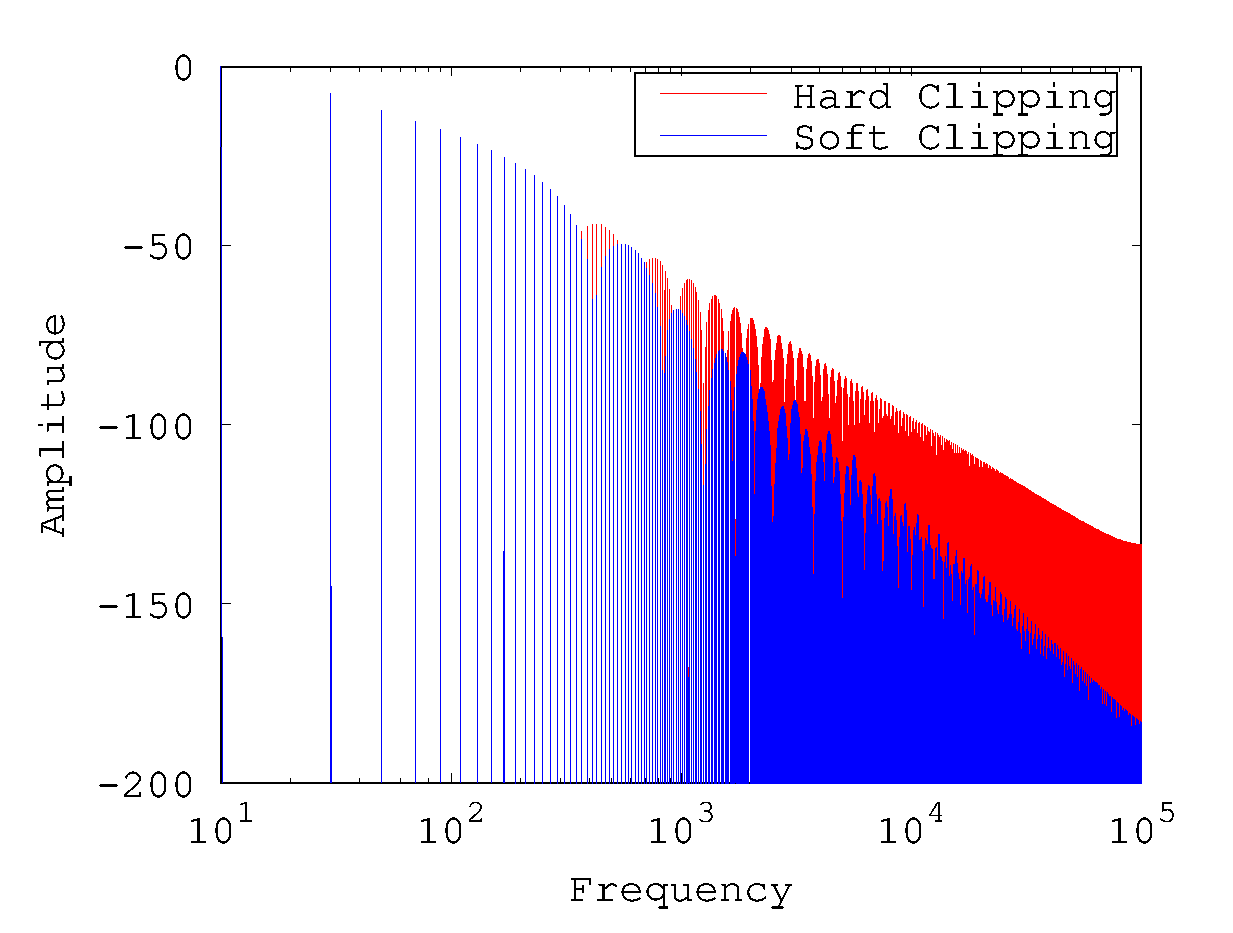
\includegraphics[width=0.6\textwidth]{chapter3/Images/ClippingSpectra.eps}
				\caption{Spectra of sinusoids clipped using Equations \ref{eq:SymmetricHardClipping} and
			                 \ref{eq:SymmetricSoftClipping}.}
				\label{fig:ClippingSpectra}
			\end{figure}

			The large amount of spectral content introduced by static nonlinearities means they are
			particularly susceptible to aliasing. Through smoothing the characteristic curve of the
			nonlinearity (making the clipper `softer') the amplitudes of generated frequencies will roll of
			more quickly. With lower levels of high order distortion the amplitudes of any aliased components
			will be reduced.

		\subsubsection*{Temporal Characteristics}
			As static nonlinearities are memoryless they can not influence the temporal evolution of signals at
			a large scale. There is a possibility to affect the attack and release times of signals slightly
			through increasing the gradient of the low amplitude section characteristic curve. As an extreme
			example consider the infinite peak clipper shown in Equation \ref{eq:InfinitePeakClipper}.

			\begin{equation}
				y[n] = \begin{cases}
					-1 & \text{if $x[n] < 0$} \\
					0 & \text{if $x[n] = 0$} \\
					1 & \text{if $x[n] > 1$}
				\end{cases}
				\label{eq:InfinitePeakClipper}
			\end{equation}
			
			Figure \ref{fig:InfinitePeakClipping} shows a signal, with attack and release sections, before and
			after infinite peak clipping. The original signal rises to it's full amplitude over two cycles and
			falls back to silence over the same time. After infinite peak clipping the attack and release have
			become instantaneous.

			\begin{figure}[h!]
				\centering
				\includegraphics[width=0.6\textwidth]{chapter3/Images/InfinitePeakClipping.eps}
				\caption{A graph showing a signal before and after infinite peak clipping.}
				\label{fig:InfinitePeakClipping}
			\end{figure}

%		\subsubsection*{Flexibility}
%			For musical signals static nonlinearities introduce a spectrally rich band of audio. The spectral
%			content of which is highly dependent on that of the input signal. The bandwidth of the new set of
%			frequencies can be easily controlled through filtering or through the techniques discussed for
%			reducing aliasing. This allows for good performance in situations where energy needs to be added to
%			a specific area of the spectrum. 
			
%		\subsubsection*{Naturalness}

	\subsection{Rectification}
	\label{sec:Excitation-Rectification}
		Rectification is a special case of static nonlinearity. Signals can be either half or full wave rectified,
		as shown in Equations \ref{eq:HalfWaveRectification} and \ref{eq:FullWaveRectification} respectively.

		\begin{equation}
			y[n] = \begin{cases}
				0 & \text{if $x[n] < 0$} \\
				x[n] & \text{otherwise}
			\end{cases}
			\label{eq:HalfWaveRectification}
		\end{equation}

		\begin{equation}
			y[n] = |x[n]|
			\label{eq:FullWaveRectification}
		\end{equation}

		\subsubsection*{Complexity}
			As with other static nonlinearities, rectifiers are very efficient. For full wave rectification
			only a single absolute value operation need be performed on each sample. Half wave rectification
			requires a comparison operation to detect negative samples before an assignment operation is
			applied.

		\subsubsection*{Homogeneity}
			One of the main advantages of rectifiers is that they are homogeneous systems. In half wave
			rectification the magnitude of negative samples is eliminated irrespective of any gain which may
			have been applied to them. In full wave rectification the absolute value of every sample is taken
			preserving their magnitude and thus any gain which has been applied.

			\note
			{
				Formal proof?
			}

		\subsubsection*{Spectral Characteristics}
			Full wave rectification can be considered as a static nonlinearity with an even characteristics
			curve. As such it only introduces even order distortion components. The Fourier coefficients of a
			rectified sine wave are shown in Equation \ref{eq:RectificationFourier}.

			\[ c_{n} = \frac{1}{2\pi} \int_{-\pi}^{\pi} |sin(x)|e^{-inx} dx \]

			\begin{equation}
				c_{n} = \begin{cases}
					\frac{2}{\pi(1 - n^{2})} & \text{when $n$ is even} \\
					0 & \text{when $n$ is odd}
				\end{cases}
				\label{eq:RectificationFourier}
			\end{equation}

			This represents all even order harmonics rolling off at approximately 12dB per octave.  As with
			other static nonlinearities rectifiers are susceptible to aliasing. The relatively shallow roll off
			of the distortion components can lead to a considerable amount of energy present in the aliased
			components of the output signal. 

			The output from a half wave rectifier has the same spectrum as that of a full wave rectifier
			but with the content of the original signal included. This can easily be shown by considering how a
			half wave rectified signal can be constructed from the original signal and a full wave rectified
			signal. Where $x(n)$, $x_{f}(n)$ and $x_{h}(n)$ represent the original signal, full wave rectified
			and half waves rectified signals respectively, their relationship can be seen in Equation
			\ref{eq:RectificationRelationship}.

			\begin{equation}
				x_{h}[n] = \frac{1}{2} \left( x_{f}[n] + x[n] \right)
				\label{eq:RectificationRelationship}
			\end{equation}

		\subsubsection*{Temporal Characteristics}
			Full wave rectifiers have no effect on the temporal characteristics of signals as all the magnitude
			of each sample is preserved. It is possible that a half wave rectifier could change the position of
			the onset of a signal by a small amount. Considering a signal which starts with a negative
			displacement. This first section of the signal would be removed, moving the onset to wherever the
			first positive displacement occurs.
			
%		\subsubsection*{Flexibility}
%			Rectifiers are useful when large amounts of even order distortion components are required. As with
%			other static nonlinearities the bandwidth of the newly introduced set of frequencies can be
%			controlled through filtering to provide more flexibility. 

%		\subsubsection*{Naturalness}

	\subsection{Integrator}
	\label{sec:Excitation-Integrator}
		Equation \ref{eq:Integrator} shows an Integrator adapted from the one described by \citet{larsen2004audio}.

		\begin{equation}
			y[n] = \begin{cases}
				0 & \text{if $x[n] > 0$ and $x[n - 1] \leq 0$} \\
				y[n - 1] + k|x[n]| & \text{otherwise}
			\end{cases}
			\label{eq:Integrator}
		\end{equation}

		Where $k$ is the integration constant, effectively setting the output gain of the system. The output signal
		is reset to 0 ofter every negative to positive zero crossing in order to prevent the sample amplitudes from
		rising indefinitely.

		\subsubsection*{Complexity}
			For each sample two comparison operations are required to detect zero crossings. This is followed
			by some simple arithmetic operations in order to integrate the signal. While this may total more
			operations than a very basic static nonlinearity it still requires very little processing power.

			Unlike static nonlinearities the integrator shown in Equation \ref{eq:Integrator} requires memory
			to store the previous output sample. 

		\subsubsection*{Homogeneity}
			Integration is a homogeneous operation. This is an advantage over certain static nonlinearities as
			though more operations are needed per sample no further work is needed to make the system
			homogeneous. If a homogeneous system is required it may be more efficient to use an integrator over
			a static nonlinearity.
		
			\note
			{
				Formal proof?
			}

		\subsubsection*{Spectral Characteristics}
			Applying Equation \ref{eq:Integrator} to a sine wave produces a signal with Fourier coefficients as
			shown in Equation \ref{eq:IntegratorFourier}.

			\[ c_{n} = \frac{kf_{s}}{2\pi} \left( \int_{0}^{\pi} (1 - cos(x))e^{-inx} dx +
							       \int_{\pi}^{2\pi} (3 + cos(x))e^{-inx} dx \right) \]

			\[ c_{-1} = - \frac{2ikf_{s}}{\pi} \]
			\[ c_{0} = 2kf_{s} \]
			\[ c_{1} = \frac{2ikf_{s}}{\pi} \]
			\begin{equation}
				c_{n} = \frac{ikf_{s}}{2\pi} \left( \frac{4n^{2} + 2e^{-i\pi n} - 2}{n^{3} - n} \right)
				\label{eq:IntegratorFourier}
			\end{equation}

			This produces all harmonics with amplitudes rolling off at approximately 6dB per octave. This
			shallow roll of make integrators very useful when a large amount of new frequency content is
			desired. Due to the shallow roll of of the distortion component's amplitudes integrators are very
			prone to aliasing.

			While integrators are homogeneous they are frequency dependant acting as low pass filters. Using
			the same integration constant a high frequency input signal will produce a lower amplitude output
			that a low frequency input. This does not affect the relatives amplitudes of frequencies in the
			output just the overall amplitude of the signal.

		\subsubsection*{Temporal Characteristics}
			Due to the inherent low pass filtering behaviour of integrators the temporal properties of
			transient signals will be altered. Attacks times will be lengthened by the attenuation of their
			high frequency components. This prevents these methods being used where it is essential that
			transients are preserved. 
			
%		\subsubsection*{Flexibility}
%			Integrators provide an efficient means to add wideband energy to the spectrum of a signal. All
%			orders of distortion are generated making this new signal spectrally dense. The bandwidth of the
%			new signal can easily be controlled through filtering improving the flexibility.

%		\subsubsection*{Naturalness}

	\subsection{Multiplier}
	\label{sec:Excitation-Multiplier}
		Multipliers are a subset of static nonlinearities in which input samples are raised to a positive integer
		power as shown in Equation \ref{eq:Multiplier}.

		\begin{equation}
			y[n] = x[n]^{h}, \quad h \in \mathbb{N}
			\label{eq:Multiplier}
		\end{equation}

		Exponential distortion extends this method by relaxing the restriction on the exponent ($h$). Allowing to
		to take any positive value. The advantages and disadvantages of this will be discussed in this section.

		\subsubsection*{Complexity}
			Being a static nonlinearity the complexity of a multiplier is very low. A single exponentiation
			operation is applied to each sample. 

		\subsubsection*{Homogeneity}
			Exponentiation is a non-homogeneous operation. Any amplitude applied to a signal before processing
			is also raised to the exponent, as shown in Equation \ref{eq:MultiplierHomogeneity}.

			\begin{equation}
				(ax[n])^{h} = a^{h}x[n]^{h}
				\label{eq:MultiplierHomogeneity}
			\end{equation}

			Unlike clippers there is no threshold parameter to change in response to the amplitude of the input
			signal. Gain stages can be added before and after the nonlinearity in order to make the systems
			response to different input amplitudes more uniform.
			
		\subsubsection*{Spectral Characteristics}
			Nonlinear processing using Equation \ref{eq:Multiplier}, in which the exponent is a positive
			integer, allows for control over the maximum order of distortion generated. The highest frequency
			present among those generated will be equal to the highest frequency in the input signal multiplied
			by the exponent. This facilitates more control over the bandwidth of the generated signal providing
			greater flexibility and minimisation of aliasing.

			If the exponent is allowed to take any positive value, control over the bandwidth of the output
			signal is lost. Non integer exponents cause higher orders of distortion to be generated. Figures
			\ref{fig:CubedSpectra} and \ref{fig:TwoAndAHalfSpectra} show the spectral effects of exponential
			distortion with integer and non integer exponents. The input signal has a fundamental frequency of
			1kHz and has energy in the first four harmonics.

			\begin{figure}[h!]
				\centering
				\includegraphics[width=0.6\textwidth]{chapter3/Images/CubedSpectra.eps}
				\caption{The spectral effects of cubing a signal with energy in its first four harmonics.}
				\label{fig:CubedSpectra}
			\end{figure}

			\begin{figure}[h!]
				\centering
				\includegraphics[width=0.6\textwidth]{chapter3/Images/RaisedToTwoAndAHalfSpectra.eps}
				\caption{The spectral effects of raising a signal with energy in its first four harmonics
					 to the power 2.5.}
				\label{fig:TwoAndAHalfSpectra}
			\end{figure}

			The highest frequency component in the original signal is 4kHz. After cubing the signal the highest
			frequency is three times this (12kHz) as seen in Figure \ref{fig:CubedSpectra}. Figure
			\ref{fig:TwoAndAHalfSpectra} shows that when the exponent is 2.5 higher frequency components are
			introduced. 

		\subsubsection*{Temporal Characteristics}
			Exponential distortion has a dynamic compression/expansion effect. For exponents greater than 1 the
			dynamics of a signal are expanded, the amplitude difference between low and high amplitude portions
			of the signal is increased. For exponents less that 1 the opposite occurs, compressing the dynamics
			of the signal. Figure \ref{fig:ExponentiationTemporalEffects} show the effects this can have on the
			attack and release portions of signals.

			\begin{figure}[h!]
				\centering
				\includegraphics[width=0.6\textwidth]{chapter3/Images/ExponentiationTemporalEffects.eps}
				\caption{The temporal effects of exponential distortion.}
				\label{fig:ExponentiationTemporalEffects}
			\end{figure}

			While the time taken for the signal to rise to or decay from maximum amplitude is not changed, the
			shape of the amplitude envelope during the attack and release portions is. 

			\note
			{ 
				Probably mention the timbral effects of this in the timbre section
				\citep{patterson1994the}.
			}

		\subsubsection*{Flexibility}
			Multipliers offer greater flexibility than the previously discussed excitation methods. Control
			over the orders of distortion introduced allows for finer shaping of a signals spectrum. The output
			of several multipliers with different exponents can be summed in order to include multiple orders
			of distortion.

			Summing multiplier outputs in this way allows for approximation of other static
			nonlinearities. A low order polynomial expression approximating the desired characteristic curve
			is calculated by linear regression as shown in Figure \ref{fig:ClippingApproximation}. The
			order of the polynomial controls the maximum order of the distortion components.

			\begin{figure}[h!]
				\centering
				\includegraphics[width=0.6\textwidth]{chapter3/Images/ClippingApproximation.eps}
				\caption{A 7\super{th} order approximation of hard clipping using linear regression.}
				\label{fig:ClippingApproximation}
			\end{figure}

			Generating characteristic curves in this way reduces the number of aliased frequencies at the cost
			of having to evaluate a more complex polynomial to calculate the output value for each sample. A
			similar approach is undertaken by \cite{fernandez-cid2001distortion} who construct characteristic
			curves from Chebyshev polynomials in order to control the highest frequencies introduced.

%		\subsubsection*{Naturalness}

	\subsection{Single Side Band Automodulation}
	\label{sec:Excitation-SSBA}
		Single sideband automodulation (SSBA) utilises the concept of single sideband modulation
		\citep{corinthios2009signals}. This allows you to apply amplitude modulation to a signal and only produce
		either the sum or difference sideband.

		A simple way to apply single sideband modulation to a signal is through construction of an analytic signal.
		An analytic signal is a complex valued signal, the real part of which is the original signal and the
		imaginary part its Hilbert transform. The analytic signal is often denoted with a subscript letter
		$a$, such that the analytic representation of the signal $x(n)$ would be denoted $x_{a}(n)$.

		\note{This Hilbert transform stuff should probably be moved elsewhere.}

		An ideal Hilbert transform alters the phase information of a signal while leaving the magnitude information
		unchanged. Any negative frequencies in the signal have their phase shifted by $\frac{\pi}{2}$ radians.  The
		phase of positive frequencies is shifted by $-\frac{\pi}{2}$ radians. The transfer function for an FIR
		implementation of a Hilbert transform is shown in Equation \ref{eq:FirHilbertTransform}.

		\begin{equation}
			H(z) = \sum_{m = -M}^{M} \frac{2}{m\pi} sin^{2} \left( \frac{m\pi}{2} \right) z^{-m}
			\label{eq:FirHilbertTransform}
		\end{equation}

		For an ideal Hilbert transform the impulse response should be infinitely long ($M = \infty$). Practicable
		approximations of an ideal Hilbert transform can be created by using a finite value for $M$. A delay of $M$
		samples must also be introduced in order to make the filter causal. As the value of $M$ is decreased this
		delay is reduced while the magnitude response of the filter deviates further from the ideal. Figure
		\ref{fig:HilbertMagnitude} shows the magnitude responses for FIR Hilbert transform filters with $M = 11$
		and $M = 101$. The filters have a bandpass response with some ripple in the pass band. As $M$ is increased
		the bandwidth of the passband is increased and the ripple reduced. The phase response of these filters
		remains ideal no matter the value of $M$, as evidenced by Figure \ref{fig:HilbertPhase}.

		\begin{figure}[h!]
			\centering
			\includegraphics[width=0.6\textwidth]{chapter3/Images/HilbertMagnitudeResponses.eps}
			\caption{Magnitude responses of FIR Hilbert transform filter with different orders.}
			\label{fig:HilbertMagnitude}
		\end{figure}

		\begin{figure}[h!]
			\centering
			\includegraphics[width=0.6\textwidth]{chapter3/Images/HilbertPhaseResponses.eps}
			\caption{Phase responses of FIR Hilbert transform filters with different orders.}
			\label{fig:HilbertPhase}
		\end{figure}

		When using Equation \ref{eq:FirHilbertTransform} a compromise needs to be made between the tolerable amount
		of delay and the accuracy of the filter's magnitude response. Increasing $M$ will give a more accurate
		filter but introduce more delay and increase the complexity of the filter. More efficient implementations
		can be build using IIR filters if some of the properties of an ideal Hilbert transform are disregarded.

		\citet{oppenheim2014discrete} suggest constructing a phase splitter. Processing audio with two parallel
		allpass IIR filters the phase responses of which differ from each other by $\frac{\pi}{2}$ radians for a
		large proportion of the spectrum. While this is not strictly a Hilbert transform it creates two signals
		which can be used as the real and imaginary part of an analytic signal. \citet{niemitalo2003hilbert}
		provides an implementation of such a pair of filters. The phase difference between these two filters is
		seen in Figure \ref{fig:IIRHilbertPhase}.

		\begin{figure}[h!]
			\centering
			\includegraphics[width=0.6\textwidth]{chapter3/Images/IIRHilbertPhaseResponses.eps}
			\caption{The phase difference between the two allpass filters proposed by
			         \citet{niemitalo2003hilbert}.}
			\label{fig:IIRHilbertPhase}
		\end{figure}

		In single sideband automodulation the analytical representation of the input signal is multiplied with
		itself in order to generate harmonics. Equation \ref{eq:SSB} shows the $h^{\text{th}}$ order single side
		band automodulation of a signal.

		\begin{equation}
			y[n] = \Re \left( x_{a}[n]^{h} \right), \quad h \in \mathbb{N}
			\label{eq:SSB}
		\end{equation}

		\subsubsection*{Complexity}
			Compared with the harmonic excitation methods discussed previously, single side band automodulation
			has greater complexity. A Hilbert transform must be applied before a complex exponentiation
			operation for each sample. The Hilbert transform filter used must give similar response for a wide
			range of frequencies so the resulting harmonic excitation gives similar results at different
			frequencies.
			
			A high order FIR Hilbert transform filter is required to give a suitably flat magnitude response.
			A lower complexity IIR phase splitter can be used in order to reduce the computational load.
			The implementations given by \citet{niemitalo2003hilbert} consists of eight biquad filters and a
			one sample delay.
			
		\subsubsection*{Homogeneity}
			As with multipliers, SSBA is a non-homogeneous process. The amplitude envelope of the $h^{th}$
			order automodulation is the amplitude envelope of the original signal raised to the power $h$. 

			\note
			{
				Formal proof?
			}

		\subsubsection*{Spectral Characteristics}
			SSBA extends the control provided by multipliers as it constrains the minimum frequency introduced
			as well as the highest. Using Equation \ref{eq:SSB} only the upper side band (the sum frequencies)
			of the modulation is produced. The highest and lowest frequency components of the output are that
			of the input signal multiplied by the exponent. Between these two frequencies lie all the other
			harmonic and intermodulation components created. This can be seen in figure \ref{fig:SSBA3Spectra},
			which shows the results of applying $3^{rd}$ order SSBA to the signal used in Figures
			\ref{fig:CubedSpectra} and \ref{fig:TwoAndAHalfSpectra}. 			
			
			\begin{figure}[h!]
				\centering
				\includegraphics[width=0.6\textwidth]{chapter3/Images/SSBA3Spectra.eps}
				\caption{The spectral effects of applying third order SSBA to a signal with energy in its 
				         first four harmonics.}
				\label{fig:SSBA3Spectra}
			\end{figure}

			If aliasing does occur it is possible for the aliased frequency to lie outside of this bandwidth.
			The amplitude of aliased frequencies can be greatly reduced through filtering. Applying a low pass
			filter with a cutoff frequency of $\frac{f_{s}}{2h}$ prior to processing will reduce the amplitude
			of any frequency content in the input which will cause aliasing when processed.

		\subsubsection*{Temporal Characteristics}
			SSBA has similar temporal effects to a multiplier using an exponent greater that 1. The signal
			undergoes dynamic expansion changing the shape of its attack and release envelopes as shown in
			Figure \ref{fig:SSBATemporalEffects}.

			\begin{figure}[h!]
				\centering
				\includegraphics[width=0.6\textwidth]{chapter3/Images/SSBATemporalEffects.eps}
				\caption{The temporal effects of SSBA.}
				\label{fig:SSBATemporalEffects}
			\end{figure}

			The restricted bandwidth of the SSBA technique's output is also apparent from this graph. The input
			is a sinusoid with a simple amplitude envelope. The output is a sinusoid with 3 times the frequency
			and an amplitude envelope equal to that of the input cubed. This is in contrast to the effect of
			the multiplier shown in Figure \ref{fig:ExponentiationTemporalEffects} where the output signal is
			no longer sinusoidal.

%		\subsubsection*{Flexibility}
%		\subsubsection*{Naturalness}

	\subsection{Instantaneous Amplitude and Phase}
	\label{sec:Excitation-IAP}
		In this method, the instantaneous amplitude and phase (IAP) of the analytic signal are calculated. These
		values are then used to aid in the construction of harmonics. The instantaneous amplitude of the analytic
		signal is found by taking its absolute value, $|x_{a}[n]|$. The instantaneous phase is found by taking the
		complex argument of the analytic signal, $\arg(x_{a}[n])$. The instantaneous phase can then be scaled in
		order to scale the frequency content of the signal independent of its amplitude. Equation \ref{eq:IAP}
		shows the $h^{\text{th}}$ order instantaneous amplitude and phase modulation of a signal.

		\begin{equation}
			y[n] = |x_{a}[n]| \cos \left( h\arg(x_{a}[n]) \right), \quad h \in \mathbb{N}
			\label{eq:IAP}
		\end{equation}

		\subsubsection*{Complexity}
			The IAP technique requires a Hilbert transform to be performed before the harmonic generation. The
			computational load of this is the same as that for the SSBA technique, an IIR phase splitter
			implementation providing a good compromise between accuracy, complexity and delay. Once an analytic
			signal has been constructed the remaining processing is applied on a sample by sample basis. 
			
		\subsubsection*{Homogeneity}
			In the IAP method the magnitude and phase information of a signal are separated. The phase
			information is scaled in order to increase the frequency while the magnitude information is left
			unaltered. This preservation of magnitude information mean that the IAP method is a homogeneous
			system.

			\note
			{
				Formal proof?
			}
			
		\subsubsection*{Spectral Characteristics}
			In contrast to the SSBA method, the IAP method is homogeneous but provides little control over the
			bandwidth of the output when the input has multiple frequency components. Figure
			\ref{fig:IAP3Spectra} shows the spectral effects of third order IAP processing on the same signal
			used when discussing previous algorithms.

			\begin{figure}[h!]
				\centering
				\includegraphics[width=0.6\textwidth]{chapter3/Images/IAP3Spectra.eps}
				\caption{The spectral effects of applying third order IAP to a signal with energy in its 
				         first four harmonics.}
				\label{fig:IAP3Spectra}
			\end{figure}

			When multiple frequency components are present in the input signal IAP processing produces energy
			at high order distortion components. As with previous algorithms it may be necessary to upsample
			the signal before precessing to avoid aliasing of these frequencies.

		\subsubsection*{Temporal Characteristics}
			The homogeneity of the system preserves the input signals amplitude envelope. Due to this the
			temporal characteristics of signals are unaffected. This can be seen in Figure
			\ref{fig:IAPTemporalEffects}, it is apparent that the frequency of the sinusoid has been altered
			and its amplitude envelope not.

			\begin{figure}[h!]
				\centering
				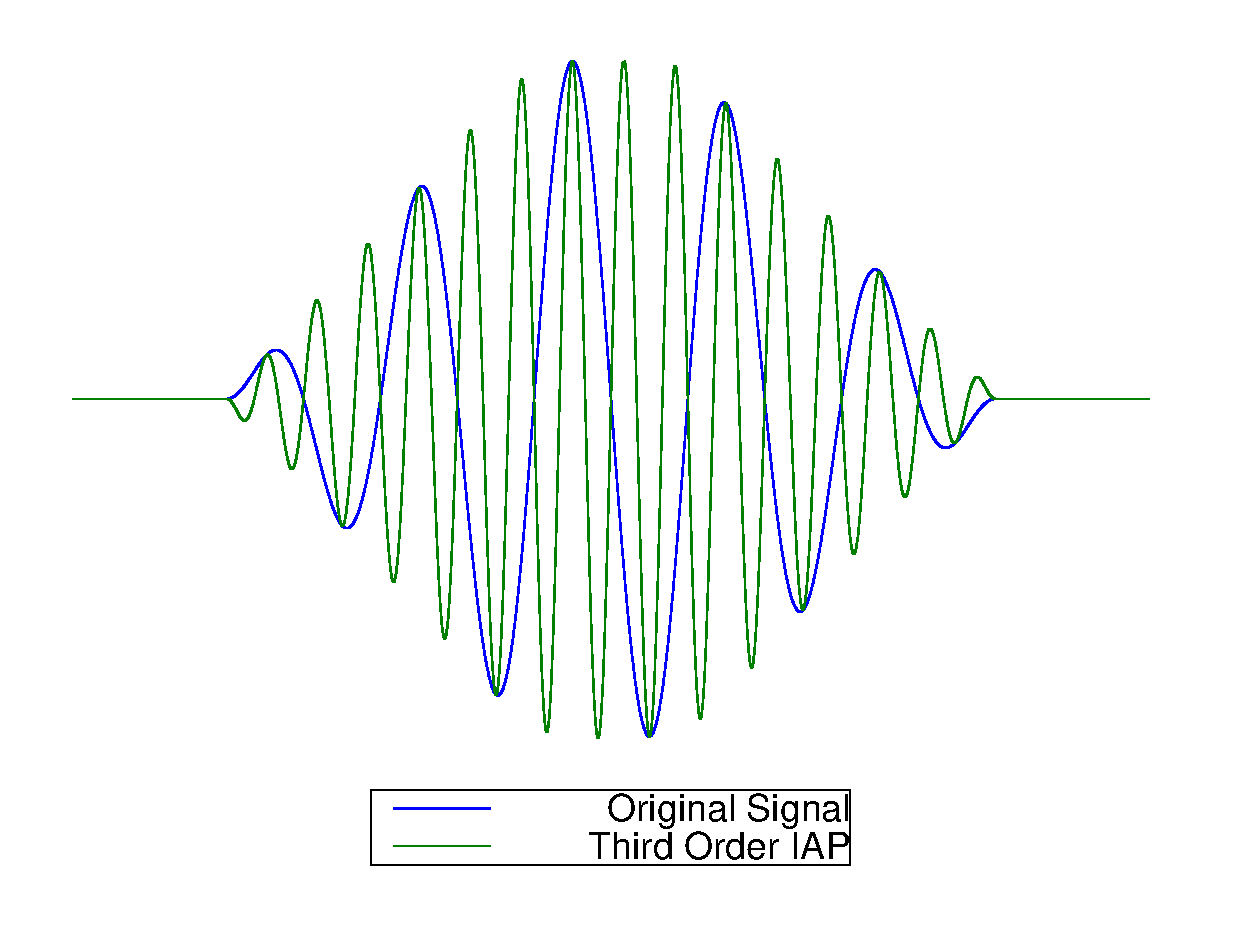
\includegraphics[width=0.6\textwidth]{chapter3/Images/IAPTemporalEffects.eps}
				\caption{The temporal effects of IAP.}
				\label{fig:IAPTemporalEffects}
			\end{figure}
			
%		\subsubsection*{Flexibility}
%		\subsubsection*{Naturalness}

	\subsection{Spectral Replication}
	\label{sec:Excitation-SpectralReplication}
		The principle behind spectral replication is to reproduce the spectral structure of a signal at higher
		frequencies as shown in Figure \ref{fig:SpectralReplication}.

		\begin{figure}[h!]
			\centering
			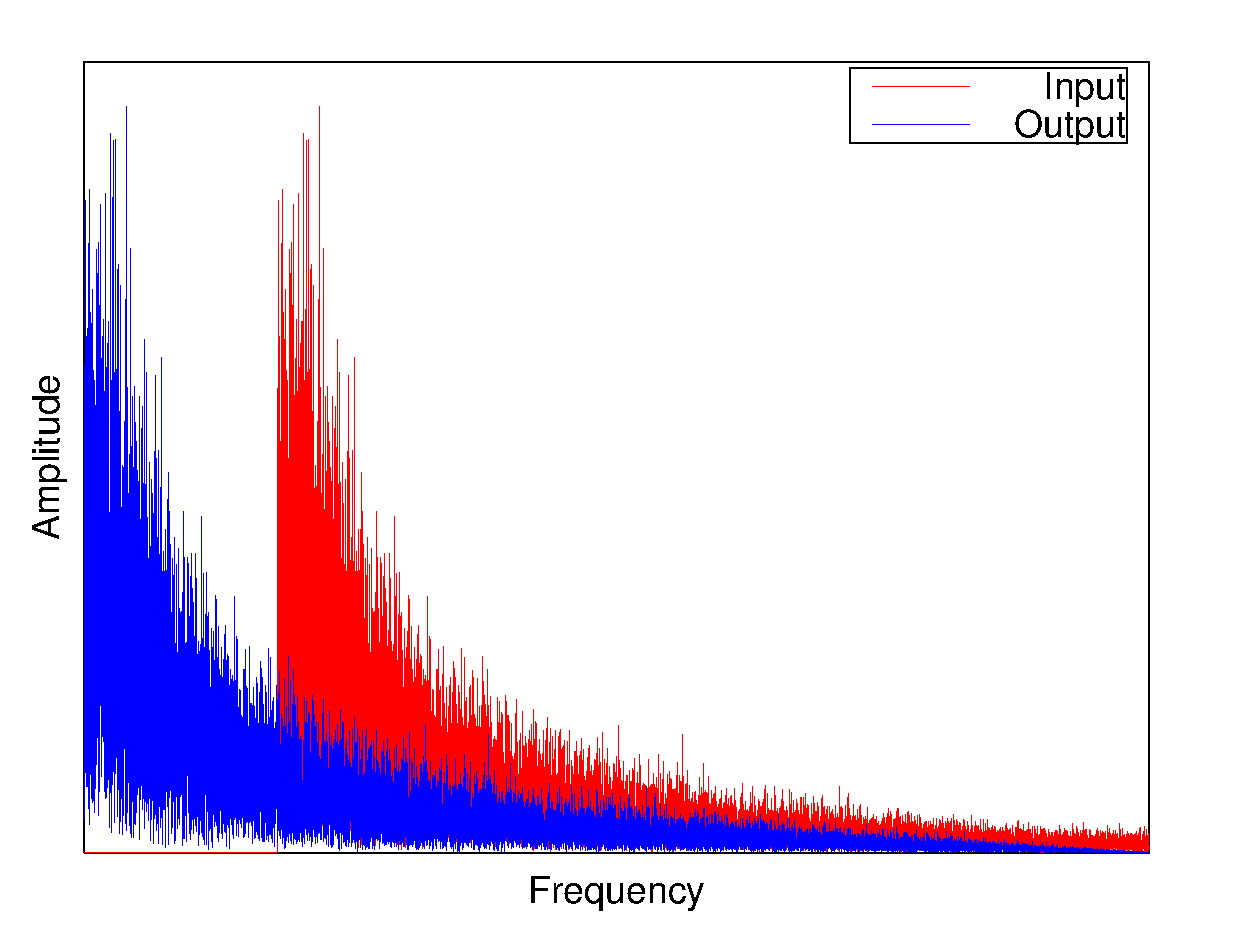
\includegraphics[width=0.6\textwidth]{chapter3/Images/SpectralReplicationSpectrum.eps}
			\caption{Reproduction of a signal at higher frequencies.}
			\label{fig:SpectralReplication}
		\end{figure}

		This spectral shift is easily implemented through the use of single side band modulation with a complex
		sinusoid as shown in Equation \ref{eq:SpectralReplication}.

		\begin{equation}
			y[n] = \Re \left( x_{a}[n] e^{2i\pi fn/ f_{s}} \right)
			\label{eq:SpectralReplication}
		\end{equation}

		Where $f$ is the amount by which the signals spectrum should be shifted.

		\subsubsection*{Complexity}
			Again, this method requires a Hilbert transform of the signal to be taken adding to the overall
			complexity of the system. After this the synthesis of a complex sinusoid needs to be carried out
			followed by the multiplication of the two complex signals on a sample by sample basis.

		\subsubsection*{Homogeneity}
			Spectral replication using Equation \ref{eq:SpectralReplication} is a homogeneous process.

			\note
			{
				Formal proof?
			}
			
		\subsubsection*{Spectral Characteristics}
			In spectral replication each frequency component is shifted by the same amount preserving the size
			of the spacings between them. This is useful for harmonic excitation of simple harmonically
			structured signals. Providing the spectrum is shifted by an integer multiple of the fundamental
			frequency any components at harmonic frequencies in the input will remain harmonic frequencies at
			the output. This process avoids the intermodulation distortion inherent to the systems discussed
			previously. 

			Due to every frequency component being shifted by an equal amount the bandwidth of the output is
			equal to that of the input. This predictability allows for easier control of the output spectrum.
			It also provides a simple method for reduction of aliasing. The highest frequency in the output
			will be that of the input plus the sift frequency $f$. Applying a low pass filter, with a cutoff
			frequency of $f_{s} - f$Hz to the input will help minimise the amplitude of any aliased frequency
			components.

		\subsubsection*{Temporal Characteristics}
			Spectral replication does not affect the temporal properties of a signal.

%		\subsubsection*{Flexibility}
%		\subsubsection*{Naturalness}

	\subsection{Spectral Folding}
	\label{sec:Excitation-SpectralFolding}
		Spectral folding uses upsampling in order to replicate parts of the spectrum at higher frequencies. In
		order for the output signal to have the same sampling frequency as the input the signal is 
		downsampled by a factor $k$ before being upsampled by the same factor. 
		
		To avoid aliasing during the downsampling phase the signal should have a low pass filter applied
		with a cutoff frequency of $\frac{f_{s}}{2k}$. Typically upsampling systems apply a low pass filter
		to remove any high frequency content introduced \citep{oppenheim2014discrete}. This is not needed for
		spectral folding as the production of high frequency energy is the desired result.

		After filtering, the downsampling and upsampling can be performed at the same time by retaining
		every $k^{th}$ sample and setting all others to zero. This is shown in Equation
		\ref{eq:SpectralFolding} where $x_{lf}[n]$ is the filtered input signal.		

		\begin{equation}
			y[n] = \begin{cases}
				x_{lf}[n] & \text{if $k \divides n$} \\
				0 & \text{otherwise}
			\end{cases}
			\label{eq:SpectralFolding}
		\end{equation}

		\subsubsection*{Complexity}
			Spectral folding using Equation \ref{eq:SpectralFolding} is relatively simple requiring only a low
			pass filter and some additional assignment operations. The complexity of the system as a whole
			largely depends on the complexity of the downsampling filter used.

		\subsubsection*{Homogeneity}
			Both downsampling and upsampling are homogeneous processes making spectral folding also
			homogeneous.

			\note
			{
				Formal proof?
			}
			
		\subsubsection*{Spectral Characteristics}
			Spectral folding with a factor $k$ results in the lowest $\frac{1}{k}$ of the input spectrum being
			repeated $k$ times in the output spectrum. Every second repetition is a mirror image of the
			original. This effect is shown in Figure \ref{fig:SpectralFolding}. 
			
			\begin{figure}[h!]
				\centering
				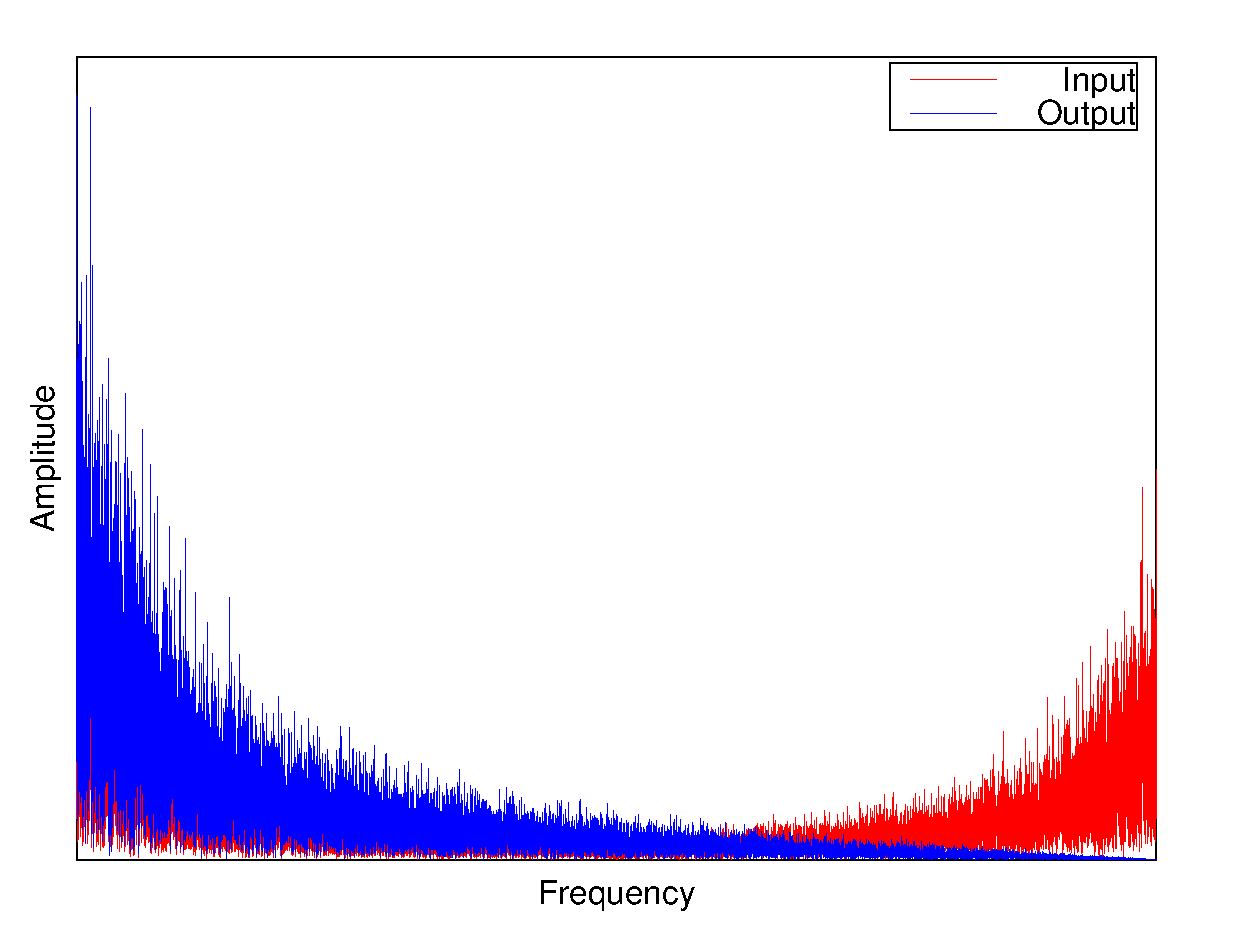
\includegraphics[width=0.6\textwidth]{chapter3/Images/SpectralFoldingSpectrum.eps}
				\caption{The spectral characteristics of spectral folding.}
				\label{fig:SpectralFolding}
			\end{figure}

			The new frequencies introduced in the output depend on the sampling rate of the signal. Unless
			$\frac{f_{s}}{2k}$ is a harmonic of the input signal there is little chance that the new
			frequencies will be harmonically related to the input.

			Other than changing the downsampling / upsampling factor, the user is given little control over the
			content of the output spectrum. The bandwidth of the output is not constricted, possibly taking up
			the entirety of the spectrum. Additional filtering is needed to shape the output spectrum as
			desired, increasing the overall complexity of the system.

		\subsubsection*{Temporal Characteristics}
			The low pass filter applied as part of the downsampling phase removes the high frequency content
			which contributes to transients in the signal. This has the effect of lengthening attack times
			similar to the effect seen in the Integrator system (Section \ref{sec:Excitation-Integrator}).

		\subsubsection*{Flexibility}
			Spectral folding is an efficient method by which to create a dense output spectrum but has many
			downsides.

%		\subsubsection*{Naturalness}

	\subsection{Spectral Stretching}
	\label{sec:Excitation-SpectralStretching}
		The principle of spectral stretching is to scale the spectrum of a signal along the frequency axis. This
		effect is shown in Figure \ref{fig:SpectralStretching}.

		\begin{figure}[h!]
			\centering
			\includegraphics[width=0.6\textwidth]{chapter3/Images/SpectralStretchingSpectrum.eps}
			\caption{The spectral characteristics of spectral stretching.}
			\label{fig:SpectralStretching}
		\end{figure}

		A typical implementation of this effect utilises a phase vocoder. The phase vocoder is an algorithm which
		allows for time stretching of a signal. It is applied by calculating the short time Fourier transform of a
		signal with a given frame and hop size. The signal is then resynthesised using a different hop size in
		order to either lengthen or shorten it. This signal can then be resampled back to the length of the
		original signal scaling the frequency content in the process. 
		
		The spectrum is scaled by a factor given in Equation \ref{eq:PhaseVocoderFactor}.

		\begin{equation}
			s = \frac{h_{s}}{h_{a}}
			\label{eq:PhaseVocoderFactor}
		\end{equation}

		Where $h_{a}$ is the hop size used when calculating the STFT and $h_{s}$ is the hop size used to
		resynthesise the signal.
		
		\subsubsection*{Complexity}
			Spectral stretching using a phase vocoder require are large amount of computation. Calculating the
			STFT involves splitting the signal into frames of which the DFT is then computed. The phase
			correction for each frame must then be computed and applied before the inverse DFT of each frame is
			taken and the frames summed back together. The resulting signal then needs to be resampled
			requiring further operations. If the scaling factor is not an integer value the resampling process
			will require additional interpolation calculations.
		
			Several steps can be taken to reduce the work needed when using a phase vocoder. The computational
			complexity of the DFT calculations can be reduced by using the fast Fourier transform
			\citep{portnoff1976implementation}. When shifting the frequencies upwards the amount of work can be
			further reduced by resampling the signal before calculating the STFT \citep{laroche1999new}. This
			way there are less frames for which the DFT need be calculated.
			
		\subsubsection*{Homogeneity}
			The phase vocoder algorithm is a homogeneous system. When processing the signal in the frequency
			domain only the phase information is altered, leaving magnitude information unchanged. 

			\note
			{
				Formal proof?
			}

		\subsubsection*{Spectral Characteristics}
			An ideal spectral stretching system would produce the result shown in Figure
			\ref{fig:SpectralStretching}. All frequency components are scaled by the same factor. For
			harmonically structured signals this has the effect of scaling the fundamental frequency.

			The phase vocoder introduces some artefacts during its operation. The process of splitting the
			signal into frames causes spectral leakage. Energy at a given frequency is spread across the nearby
			frequencies. In a signal which only has energy at harmonic frequencies, spectral stretching by an
			integer factor will produce some inharmonic content due to this effect. Spectral leakage can be
			minimised through the use of windowing functions such as the Hamming or Blackman-Harris windows. 

			Ignoring the effect of spectral leakage, the bandwidth of the output signal will be that of the
			input multiplied by the stretching factor. This allows for effective minimisation of aliasing as
			the signal can be low pass filtered before processing as done with single side band automodulation
			(Section \ref{sec:Excitation-SSBA}).
		
		\subsubsection*{Temporal Characteristics}
			A simple phase vocoder implementation produces artefacts when processing transients in a signal.
			The phase correction stage before resynthesis can have the effect of softening the attack portion.
			The exact effect had on the transient is not able to be controlled as it depends on where the
			transient lies in the STFT frame. \citet{robel2003a} proposes a method to better process transients
			with a phase vocoder. An algorithm is used to detect the presence of transients in an STFT frame.
			The phase information is then processed differently depending on the position of the transient
			within the frame.

%		\subsubsection*{Flexibility}
%		\subsubsection*{Naturalness}

\begin{landscape}
\section{Methods Comparison}
\label{sec:Excitation-Comparison}

	\begin{tabular}{|c|c|c|c|c|c|c|}
		\hline
		\bf{Method} & \bf{Complexity} & \bf{Homogeneity} & \bf{Spectral Properties} & \bf{Temporal Properties} &
		\bf{IMD} & \bf{Flexibility} \\ % & \bf{Naturalness} \\
		\hline
		Static Nonlinearity & $\mathcal{O}(n)$ & & & & & \\
		\hline
		Rectifier & $\mathcal{O}(n)$ & & & & & \\
		\hline
		Integrator & $\mathcal{O}(n)$ & & & & & \\
		\hline
		Multiplier & $\mathcal{O}(n)$ & & & & & \\
		\hline
		SSBA & $\mathcal{O}(n)$ & & & & & \\
		\hline
		IAP & $\mathcal{O}(n)$ & & & & & \\
		\hline
		Spectral Replicator & $\mathcal{O}(n)$ & & & & & \\
		\hline
		Spectral Mirror & $\mathcal{O}(n)$ & & & & & \\
		\hline
		Spectral Stretch & $\mathcal{O}(n\log{n})$ Assuming FFT used & & & & & \\
		\hline
	\end{tabular}

\end{landscape}

\section{Key Findings}
	\note
	{
		Conclude the chapter.
	}


%\section{Evaluating Excitation Methods}
%\label{sec:FeatureControl-MethodEvaluation}
%
%	\note{Homogeneity a la DAFx paper.
%	      Flexibility introduced by allowing single harmonic control a la SMC paper}
%
%	Several harmonic excitation methods were discussed in Section \ref{sec:Excitation-Methods}. When applied to the 
%	task of controlling specific audio features each of these methods has its own advantages and disadvantages.
%
%	\subsection{Homogeneity}
%	\label{sec:FeatureControl-Homogeneity}
%
%		\subsubsection*{Static Nonlinearities}		
%			As previously mentioned simple static nonlinearities are very susceptible to change in input 
%			amplitude. \citet{deman2014adaptive} counteract this issue by having the clipping threshold adapt 
%			to changes in the RMS amplitude of the input. The user is then provided with a `relative threshold' 
%			parameter on which the same setting should give similar perceptual results no matter what the input 
%			amplitude.
%
%			\note{Talk about the issues with static nonlinearities raised in \citet{enderby2012harmonic}}
%
%		\subsubsection*{Bandwidth Extension}
%			\note{Spectral mirroring, stretching and replication are all homogeneous.}
%			
%		\subsubsection*{Single Harmonic Generation}
%			Using single sideband automodulation the proportion of new frequency components in the output 
%			signal increases as the input amplitude increases. The instantaneous amplitude and phase and phase 
%			vocoder techniques are more robust in this respect.
%
%	\subsection{Flexibility}
%	\label{sec:FeatureControl-Flexibility}
%
%		\note{Flexibility is provided by individual harmonic generation \citep{enderby2013methods}}	
%
%	\subsection{Complexity}
%	\label{sec:FeatureControl-Complexity}
%		
%		\note{It is advantageous to use an algorithm that will create accurate harmonics with little analysis.
%		      Most methods don't rely on knowing the fundamental in order to generate harmonics. Spectral
%		      shifting on the other hand does.}
%
%		\note{Most of the algorithms can be easily improved through the use of a low pass filter, increasing
%	             complexity.}

\chapter{Subjective Timbre Evaluation}
\label{chap:ListeningTests}
	\todo{Come up with a better name for this chapter.}

\section{Production Environment Timbre Evaluation} % this name will probably change
\label{sec:ListeningTests-DAWBasedTimbreEvaluation}
The perceptual listening test methodologies discussed in Section \ref{sec:Timbre-ListeningTests} rely on the participants
performing a certain set of tasks. While this structure helps to reduce the number of variables in an experiment it does not
necessarily reflect the way audio is treated in a production environment.

A new methodology has been developed in which the analysis of timbre is introduced into a typical music production workflow
causing minimal interruption to the producer. This methodology aims to answer the question "What terms do music producers
use to describe the timbral transformations they apply to audio during the creation of music?". 

This section will detail what the typical production workflow is and how semantic information can be gathered.

	\subsection{Music Production Workflow}
		\todo{Find some references for this section. Probably mixing engineers handbook or something.}

		The music production workflow has four main stages:

		\begin{itemize}
			\item Recording
			\item Editing
			\item Mixing
			\item Mastering
		\end{itemize}

		At every stage of this process semantic descriptors are often used to communicate the desired timbral
		qualities of the audio. For instance one my ask that a certain microphone be used because of the `warmth' it
		adds to the recorded sound. During the mixing and mastering stages audio processing effects are applied to
		shape the timbre further.  These stages will be the focus of this section as the aim of this thesis is to
		improve the intuitiveness of these effects.

		Historically audio effects were pieces of electronic hardware through which an audio signal is passed.
		Modern music production techniques utilise Digital Audio Workstation (DAW) software. This software enables
		users to record, edit and mix multiple tracks of audio using a computer. 
		
	\subsection{Analysis of Timbre Inside the DAW}
		An ideal way to collect timbral information during music production would be to have the DAW analyse the
		audio tracks used and production techniques applied. Information which could be gathered directly from the
		DAW, with no extra input from the user, includes:

		\begin{itemize}
			\item Information about the audio processing chain:
			\begin{itemize}
				\item The effects applied to each track.
				\item The order in which these effects are applied.
				\item The parameter settings of these effects.
			\end{itemize}

			\item Features of the audio signal at every stage in the processing chain.
		\end{itemize}

		Additional information can be gathered by prompting the user for input:

		\begin{itemize}
			\item The genre of music being produced.
			\item The content of the separate audio tracks (what instruments etc.).
			\item Semantic terms which describe the timbral transformations applied by each audio
			      effect.
		\end{itemize}

		Achieving this would require the creation of a new DAW. This would be impractical for the current research.
		DAWs are very comprehensive software packages which perform many more tasks than the application of effects
		to audio (project management, audio editing functionality etc.). A lot of effort would be expended in
		implementing these features before any timbral data could be collected.  Music producers also tend to have a
		preferred DAW with which they work most fluidly. Convincing producers to use a new DAW, for the purposes of
		research, would be a difficult task.

		Third party developers can produce extensions to DAWs known as plug-ins. Plug-Ins provide additional audio
		processing functionality to the DAW environment. They can optionally expose their own parameters which users
		can adjust to achieve their desired effect. There are several different formats in which audio plug-ins can
		be distributed (VST, AU etc.). Most of the commonly used DAWs support plug-ins in one or more of these
		formats.

		Audio plug-ins provide a good platform to allow producers to provide semantic terms and audio feature
		information from within their preferred DAW. As part of this research a suite of audio plug-ins which
		extract this information have been developed. They have been release under the title Semantic Audio Feature
		Extraction (SAFE) Plug-Ins.

	\subsection{SAFE Plug-Ins}
		The SAFE plug-ins consist of four commonly used audio effects: Equaliser, Distortion, Compressor and Reverb.
		As part of the plug-ins's interface the user has the option to save semantic terms. The interface for the
		SAFE Distortion is shown in Figure \ref{fig:SAFE-Distortion}. Upon saving terms the plug-in will analyse the
		audio at its inputs and outputs. When the analysis is completed the results are stored, containing:

		\begin{itemize}
			\item The users description of the timbre.
			\item The plug-in's current parameter settings.
			\item The features of the audio before and after processing.
			\item Some additional data about the user and the track being worked on.
			\begin{itemize}
				\item The genre.
				\item The instrument.
				\item The users age.
				\item The users location.
				\item The users primary language.
				\item The number of year experience the user has in music production.
			\end{itemize}
		\end{itemize}

		\begin{figure}[h!]
			\centering
			\includegraphics[width=0.8\textwidth]{chapter4/Images/SAFEDistortion.png}
			\caption{The Interface for the SAFE Distortion Plug-In}
			\label{fig:SAFE-Distortion}
		\end{figure}

		The LibXtract library \citep{bullock2007libxtract} is used in the analysis of the audio. Every scalar
		feature available within LibXtract is calculated along with the MFCCs and Bark Band Coefficients. In total
		five seconds of audio is analysed in frames of 4096 samples each.

		\note{Why 4096 samples? The real reason is because LibXtract works better that way. Will that cut the
		mustard?}

		One disadvantage in using plug-ins is that they cannot gather information about the processing chain they
		may be a part of. The timbral transformation the user is describing may be the result of several effects
		working together. This can be mitigated somewhat by asking users to describe only the effect the plug-in in
		question is providing.

		The SAFE plug-ins also suffer from the same issues other distributed tests do. The researcher forfeits
		control over the listening environment in order to gather results from a much larger sample of people. In
		fact they provide even lest control that methodologies like that used in the Social EQ project
		\citep{cartwright2013socialeq} in that the choice of audio samples being used is decided by the test
		subject. 

\section{Analysis}
\label{sec:ListeningTests-Analysis}

	\begin{figure}[h!]
		\centering
		\subfloat[Individual Transforms]
		{
			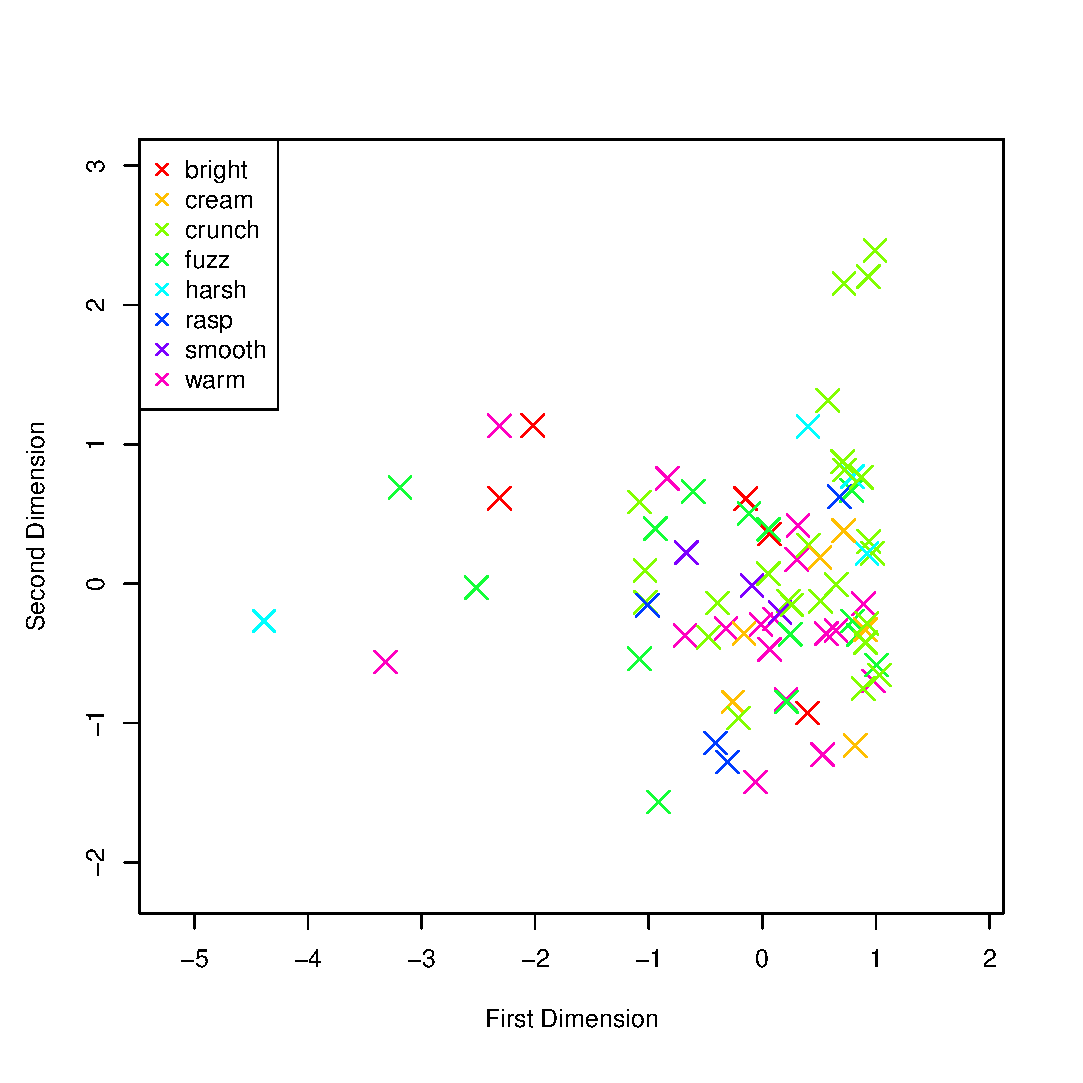
\includegraphics[width=0.45\textwidth]{chapter4/Images/DistortionProcessedMDS.eps}
			\label{fig:DistortionProcessedMDS}
		}
		\qquad
		\subfloat[Descriptor Centroids]
		{
			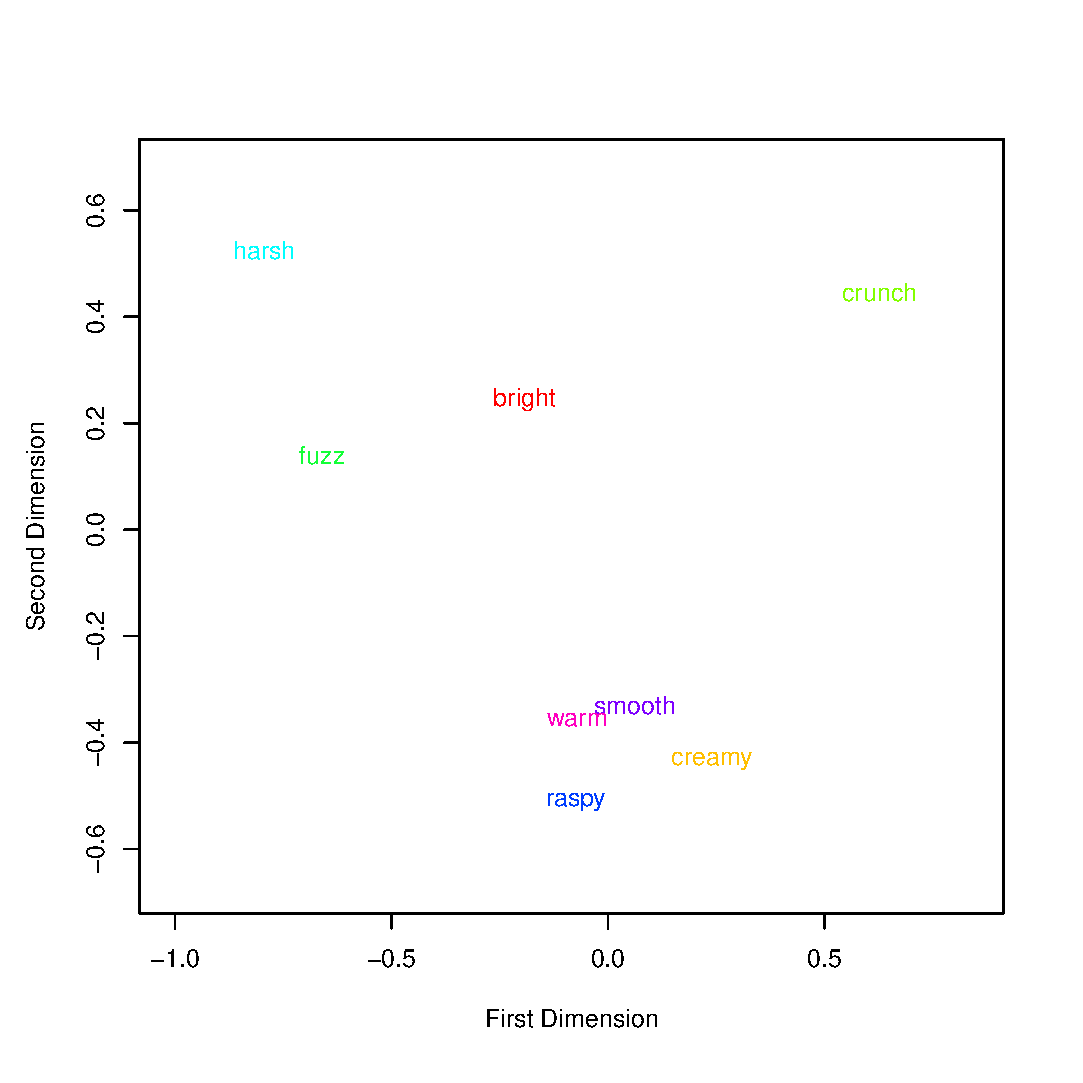
\includegraphics[width=0.45\textwidth]{chapter4/Images/DistortionProcessedCentroidsMDS.eps}
			\label{fig:DistortionProcessedCentroidsMDS}
		}
		\caption{Timbre Space for the Processed Features form the Distortion.}
		\label{fig:DistortionProcessedMDSs}
	\end{figure}

	\begin{table}[h!]
		\centering
		\begin{tabular}{|c|c|c|}
			\hline
			\bf{Feature} & \bf{Correlation} & \bf{p-value} \\
			\hline
			\hline
			Irregularity K & -0.981702638254498 & 5.86525860866353e-37 \\
			\hline
			Peak Irregularity K & -0.962036042628834 & 2.73321934750131e-29 \\
			\hline
			Bark Coefficient 6 & -0.959036054870656 & 1.70190172876899e-28 \\
			\hline
			Peak Spectral Kurtosis & -0.940033366324044 & 1.55053342301828e-24 \\
			\hline
			Bark Coefficient 7 & -0.936553028504178 & 5.93192971807379e-24 \\
			\hline
			Harmonic Irregularity K & -0.933019146143437 & 2.14810473054194e-23 \\
			\hline
			Harmonic Spectral Kurtosis & -0.924326438294474 & 3.85764808897598e-22 \\
			\hline
			Bark Coefficient 5 & -0.922957072163232 & 5.89092885576859e-22 \\
			\hline
			Peak Spectral Skewness & -0.920984402717623 & 1.06945158126544e-21 \\
			\hline
			Bark Coefficient 8 & -0.914782358316355 & 6.33230467348598e-21 \\
			\hline
		\end{tabular}
		\caption{Significant Features for Dimension 1 of the Timbre Spaces Shown in Figure 
			 \ref{fig:DistortionProcessedMDSs}.}
		\label{tab:DistortionProcessedFeaturesDim1}
	\end{table}

	\begin{table}[h!]
		\centering
		\begin{tabular}{|c|c|c|}
			\hline
			\bf{Feature} & \bf{Correlation} & \bf{p-value} \\
			\hline
			\hline
			Spectral Centroid & 0.934357264112107 & 0 \\
			\hline
			Spectral Roll Off & 0.920245205497915 & 0 \\
			\hline
			MFCC 1 & -0.896491813212876 & 5.98001677533564e-19 \\
			\hline
			Spectral Slope & 0.883921167187462 & 0 \\
			\hline
			Peak Spectral Standard Deviation & 0.85800083369724 & 8.88178419700125e-16 \\
			\hline
			Harmonic Spectral Standard Deviation & 0.856326749640604 & 1.11022302462516e-15 \\
			\hline
			Harmonic Spectral Centroid & 0.847853863903556 & 4.21884749357559e-15 \\
			\hline
			Peak Spectral Centroid & 0.846379278425876 & 5.10702591327572e-15 \\
			\hline
		\end{tabular}
		\caption{Significant Features for Dimension 2 of the Timbre Spaces Shown in Figure 
			 \ref{fig:DistortionProcessedMDSs}.}
		\label{tab:DistortionProcessedFeaturesDim2}
	\end{table}

	\begin{figure}[h!]
		\centering
		\subfloat[Individual Transforms]
		{
			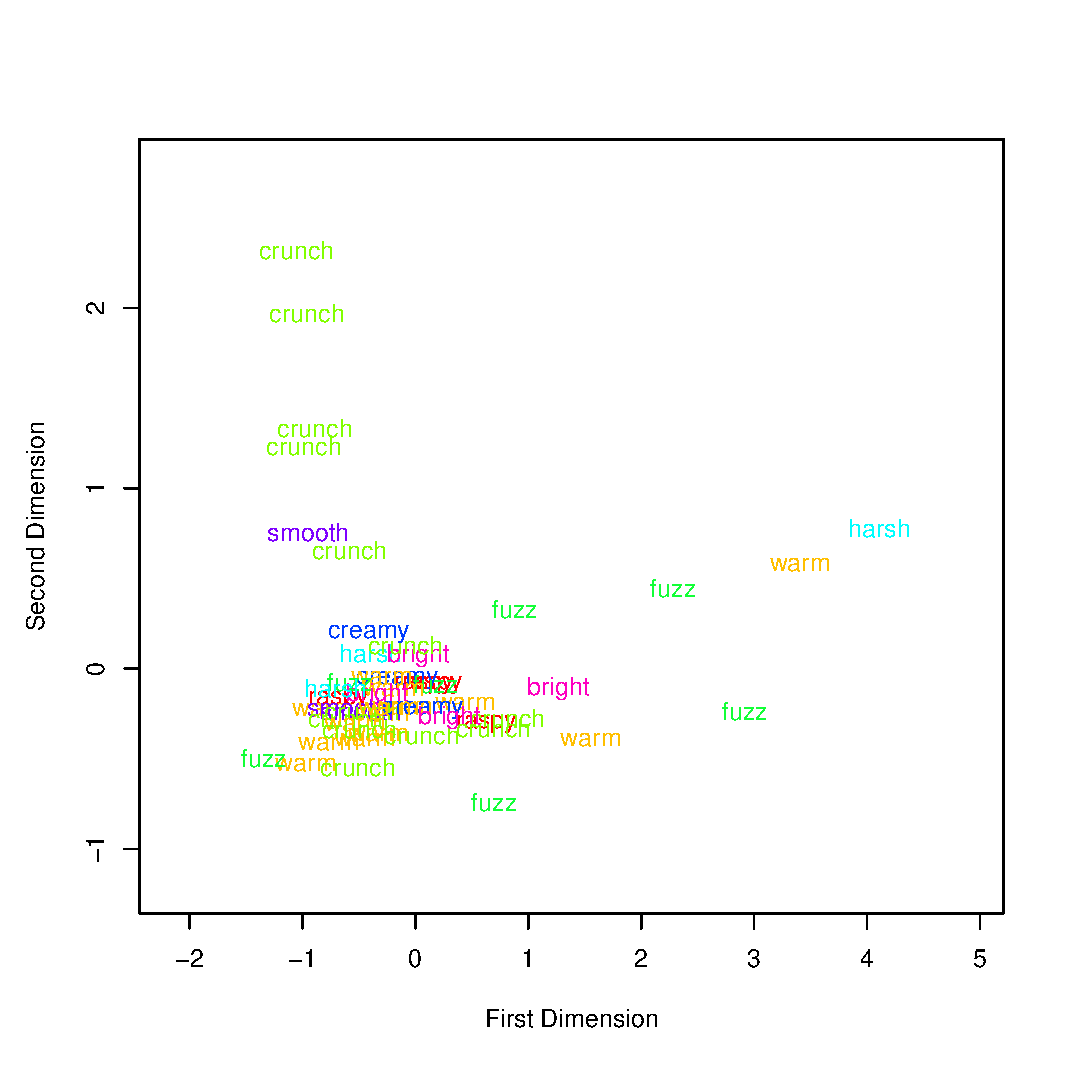
\includegraphics[width=0.45\textwidth]{chapter4/Images/DistortionDifferenceMDS.eps}
			\label{fig:DistortionDifferenceMDS}
		}
		\qquad
		\subfloat[Descriptor Centroids]
		{
			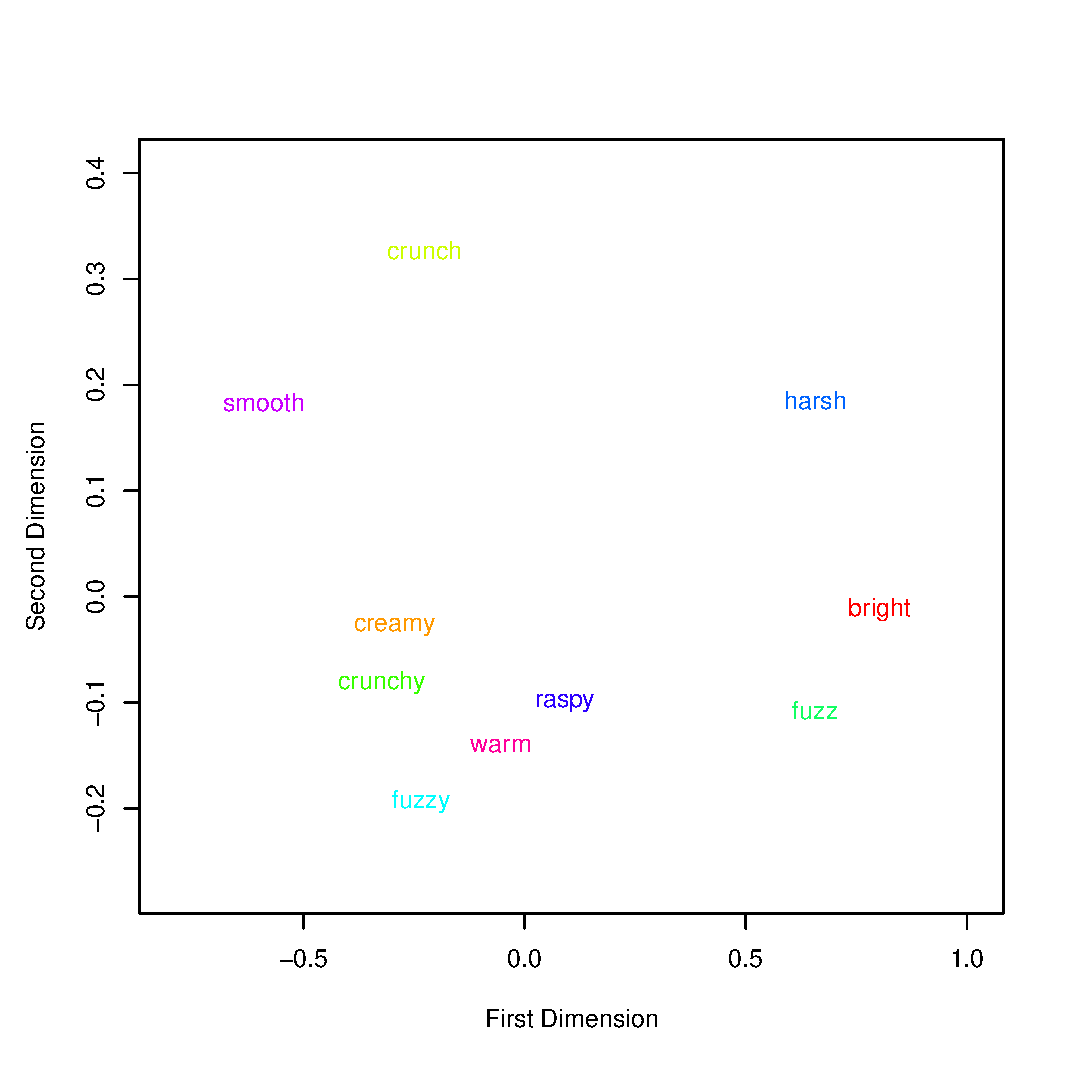
\includegraphics[width=0.45\textwidth]{chapter4/Images/DistortionDifferenceCentroidsMDS.eps}
			\label{fig:DistortionDifferenceCentroidsMDS}
		}
		\caption{Timbre Space for the Feature Differences form the Distortion.}
		\label{fig:DistortionDifferenceMDSs}
	\end{figure}

	\begin{table}[h!]
		\centering
		\begin{tabular}{|c|c|c|}
			\hline
			\bf{Feature} & \bf{Correlation} & \bf{p-value} \\
			\hline
			\hline
			Irregularity K & -0.985498074073924 & 2.05802067103551e-39 \\
			\hline
			Peak Irregularity K & -0.965585436473341 & 2.57014502660263e-30 \\
			\hline
			Bark Coefficient 6 & -0.95894018547053 & 1.8002297365022e-28 \\
			\hline
			Bark Coefficient 7 & -0.957021574844167 & 5.39083077911368e-28 \\
			\hline
			Bark Coefficient 15 & -0.952417240055253 & 6.18694971512614e-27 \\
			\hline
			Bark Coefficient 8 & -0.951360019811739 & 1.04712187507916e-26 \\
			\hline
			Bark Coefficient 9 & -0.951137188781872 & 1.16818996425268e-26 \\
			\hline
			Harmonic Irregularity K & -0.949155160917441 & 3.02442464624862e-26 \\
			\hline
			Bark Coefficient 10 & -0.937968421097708 & 3.46968829494617e-24 \\
			\hline
			Bark Coefficient 5 & -0.934441590399684 & 1.29078670910454e-23 \\
			\hline
		\end{tabular}
		\caption{Significant Features for Dimension 1 of the Timbre Spaces Shown in Figure 
			 \ref{fig:DistortionDifferenceMDSs}.}
		\label{tab:DistortionDifferenceFeatures}
	\end{table}

	\begin{table}[h!]
		\centering
		\begin{tabular}{|c|c|c|}
			\hline
			\bf{Feature} & \bf{Correlation} & \bf{p-value} \\
			\hline
			\hline
			Spectral Variance & -0.875525916695384 & 4.27315930700177e-17 \\
			\hline
			Spectral Roll Off & -0.8728405861589 & 6.98033103314871e-17 \\
			\hline
			Harmonic Spectral Centroid & -0.868256190058225 & 1.57333943755696e-16 \\
			\hline
			Harmonic Spectral Standard Deviation & -0.865564070871415 & 2.50031776893959e-16 \\
			\hline
			Peak Spectral Centroid & -0.850640310222172 & 2.752907039677e-15 \\
			\hline
			Spectral Centroid & -0.843402134079256 & 8.0379337150603e-15 \\
			\hline
			Peak Spectral Standard Deviation & -0.822865543302491 & 1.28007959107212e-13 \\
			\hline
			Peak Spectral Variance & -0.817293786410897 & 2.55259503107424e-13 \\
			\hline
			Harmonic Spectral Variance & -0.812345974117126 & 4.62139755362114e-13 \\
			\hline
		\end{tabular}
		\caption{Significant Features for Dimension 2 of the Timbre Spaces Shown in Figure 
			 \ref{fig:DistortionDifferenceMDSs}.}
		\label{tab:DistortionDifferenceFeatures}
	\end{table}

	\begin{figure}[h!]
		\centering
		\subfloat[Individual Transforms]
		{
			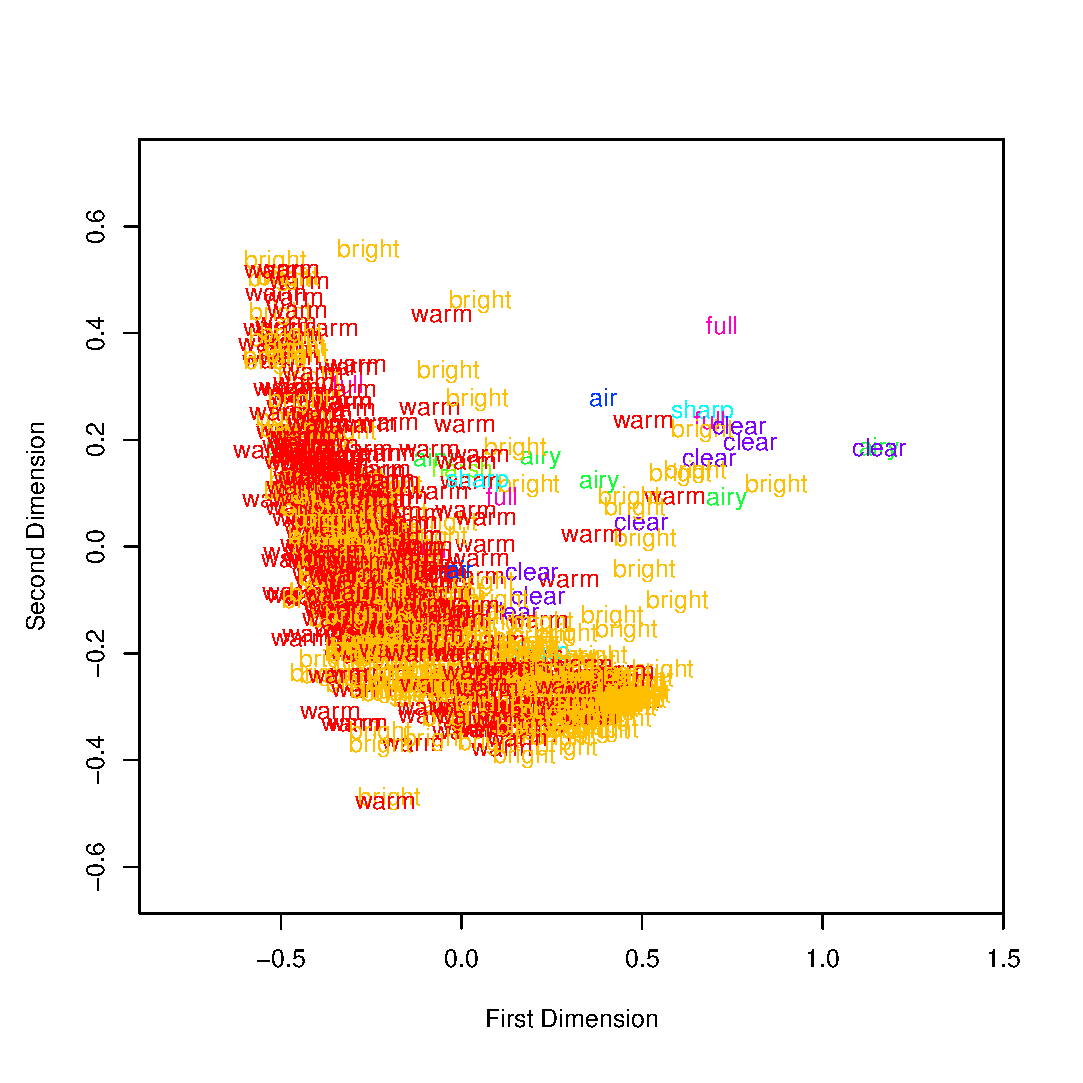
\includegraphics[width=0.45\textwidth]{chapter4/Images/EqualiserProcessedMDS.eps}
			\label{fig:EqualiserProcessedMDS}
		}
		\qquad
		\subfloat[Descriptor Centroids]
		{
			\includegraphics[width=0.45\textwidth]{chapter4/Images/EqualiserProcessedCentroidsMDS.eps}
			\label{fig:EqualiserProcessedCentroidsMDS}
		}
		\caption{Timbre Space for the Processed Features form the Equaliser.}
		\label{fig:EqualiserProcessedMDSs}
	\end{figure}

	\begin{table}[h!]
		\centering
		\begin{tabular}{|c|c|c|}
			\hline
			\bf{Feature} & \bf{Correlation} & \bf{p-value} \\
			\hline
			\hline
			Peak Tristimulus 2 & 0.855583627112928 & 0 \\
			\hline
			Spectral Crest & 0.846391686145526 & 0 \\
			\hline
			Harmonic Tristimulus 2 & 0.843557935487663 & 0 \\
			\hline
			Harmonic Spectral Standard Deviation & -0.827375175520425 & 1.94505570441165e-223 \\
			\hline
			Peak Spectral Standard Deviation & -0.82480168108147 & 7.20182231471735e-221 \\
			\hline
			Bark Coefficient 17 & -0.812395528135387 & 4.72470887847481e-209 \\
			\hline
			Bark Coefficient 14 & -0.806923230960388 & 4.07779342479812e-204 \\
			\hline
			Peak Spectral Centroid & -0.806540090277105 & 8.91420489743429e-204 \\
			\hline
			Harmonic Spectral Centroid & -0.803467926387208 & 4.42924954070955e-201 \\
			\hline
		\end{tabular}
		\caption{Significant Features for Dimension 1 of the Timbre Spaces Shown in Figure 
			 \ref{fig:EqualiserProcessedMDSs}.}
		\label{tab:EqualiserProcessedFeaturesDim1}
	\end{table}

	\begin{table}[h!]
		\centering
		\begin{tabular}{|c|c|c|}
			\hline
			\bf{Feature} & \bf{Correlation} & \bf{p-value} \\
			\hline
			\hline
			Spectral Skewness & 0.81909614086231 & 0 \\
			\hline
			Spectral Kurtosis & 0.80093620277201 & 0 \\
			\hline
		\end{tabular}
		\caption{Significant Features for Dimension 2 of the Timbre Spaces Shown in Figure 
			 \ref{fig:EqualiserProcessedMDSs}.}
		\label{tab:EqualiserProcessedFeaturesDim2}
	\end{table}

	\begin{figure}[h!]
		\centering
		\subfloat[Individual Transforms]
		{
			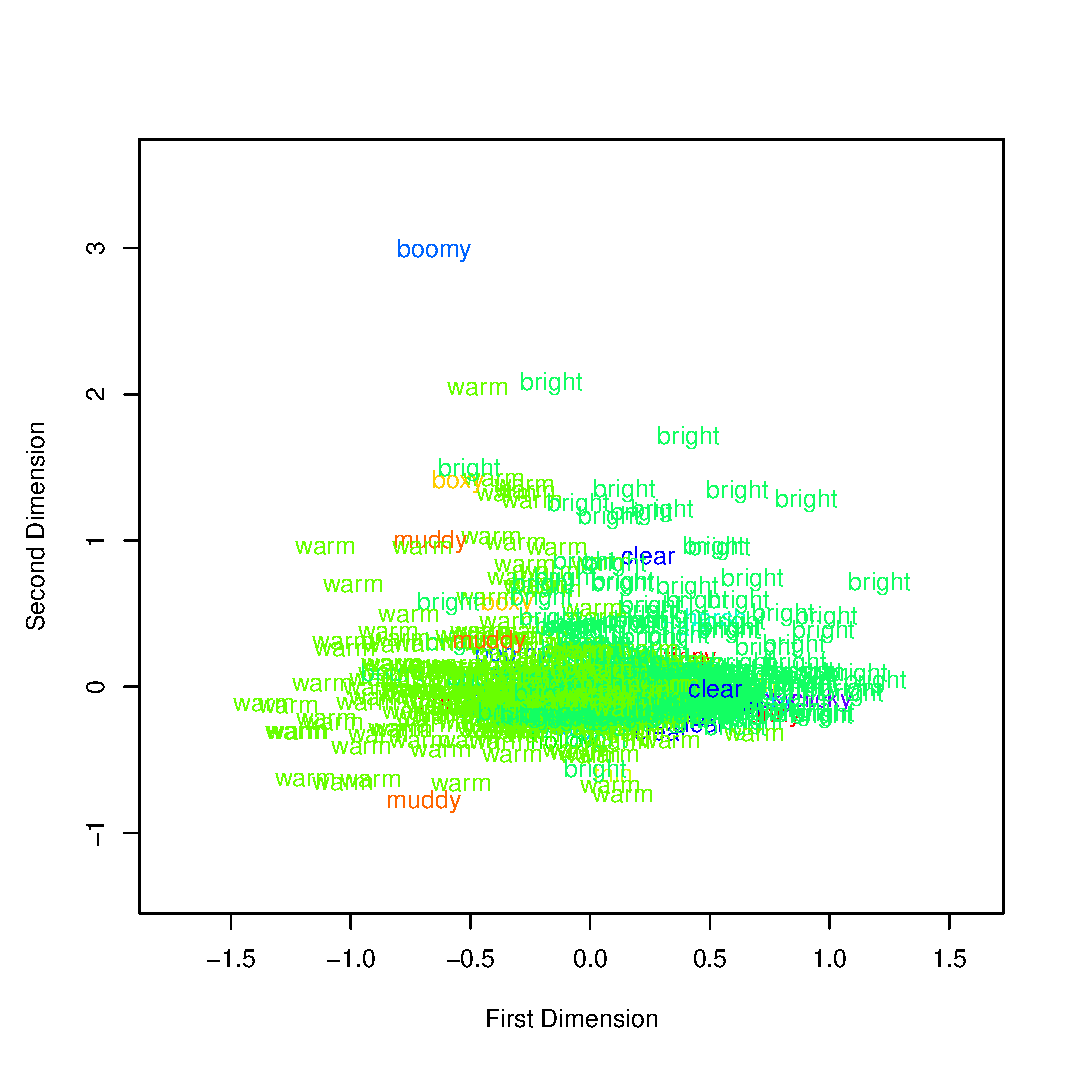
\includegraphics[width=0.45\textwidth]{chapter4/Images/EqualiserDifferenceMDS.eps}
			\label{fig:EqualiserDifferenceMDS}
		}
		\qquad
		\subfloat[Descriptor Centroids]
		{
			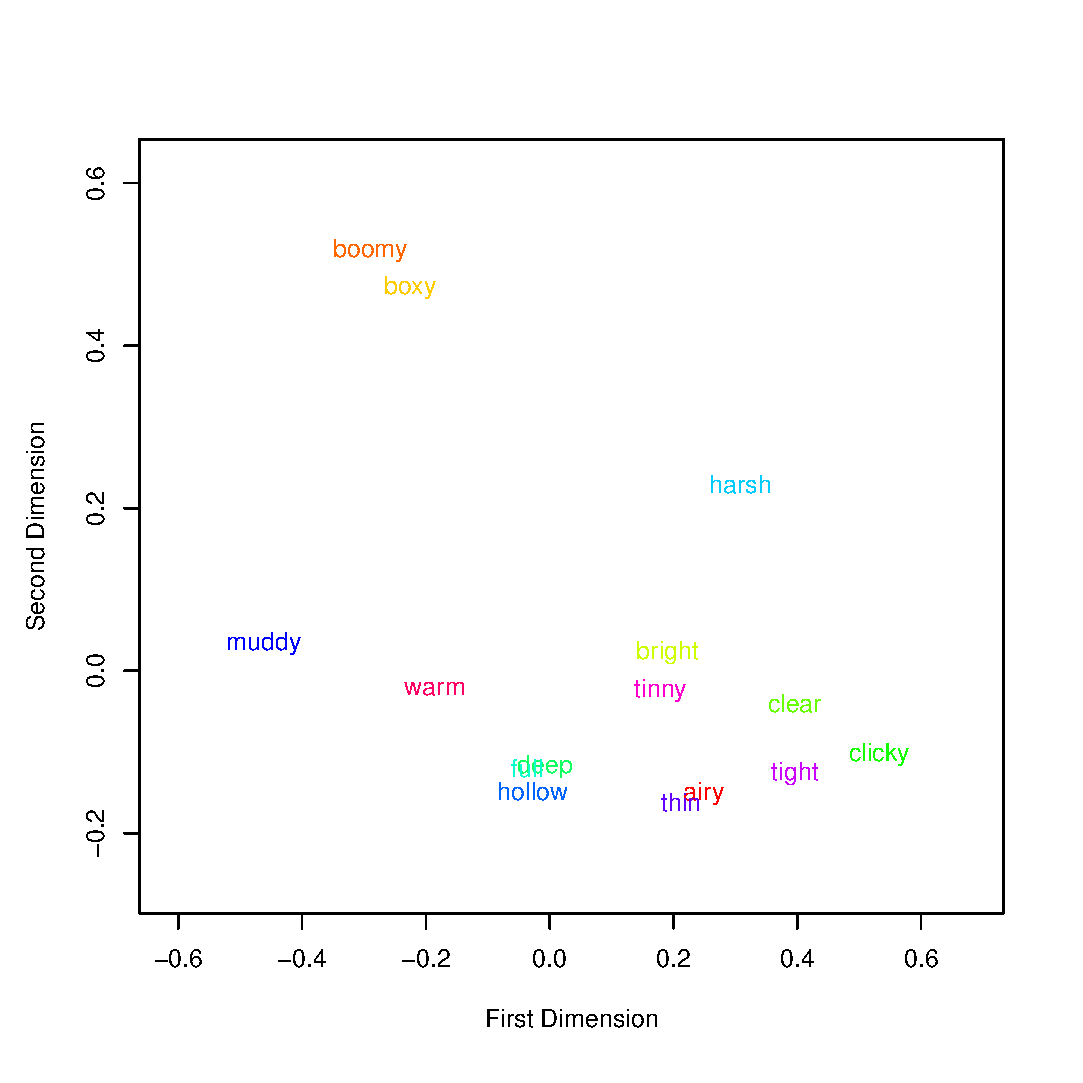
\includegraphics[width=0.45\textwidth]{chapter4/Images/EqualiserDifferenceCentroidsMDS.eps}
			\label{fig:EqualiserDifferenceCentroidsMDS}
		}
		\caption{Timbre Space for the Feature Differences form the Equaliser.}
		\label{fig:EqualiserDifferenceMDSs}
	\end{figure}

	\begin{table}[h!]
		\centering
		\begin{tabular}{|c|c|c|}
			\hline
			\bf{Feature} & \bf{Correlation} & \bf{p-value} \\
			\hline
			\hline
			Peak Tristimulus 2 & -0.890277830827284 & 3.45856612780454e-303 \\
			\hline
			Noisiness & -0.88597695501459 & 2.88937242814623e-296 \\
			\hline
			Harmonic Tristimulus 2 & -0.885741541888379 & 6.78585002438152e-296 \\
			\hline
			Harmonic Tristimulus 1 & -0.853307554457384 & 2.14548358937076e-251 \\
			\hline
			Peak Tristimulus 1 & -0.849822882281384 & 2.91473980458935e-247 \\
			\hline
			Fundamental & -0.816606742868406 & 1.74533328383416e-212 \\
			\hline
		\end{tabular}
		\caption{Significant Features for Dimension 1 of the Timbre Spaces Shown in Figure 
			 \ref{fig:EqualiserDifferenceMDSs}.}
		\label{tab:EqualiserDifferenceFeatures}
	\end{table}

	\begin{table}[h!]
		\centering
		\begin{tabular}{|c|c|c|}
			\hline
			\bf{Feature} & \bf{Correlation} & \bf{p-value} \\
			\hline
			\hline
			Irregularity K & 0.966464851638525 & 0 \\
			\hline
			Spectral Skewness & 0.942017154084719 & 0 \\
			\hline
			Spectral Kurtosis & 0.926960543352505 & 0 \\
			\hline
			Peak Irregularity K & 0.923930211100233 & 0 \\
			\hline
			Harmonic Irregularity K & 0.87430845721457 & 0 \\
			\hline
			Harmonic Spectral Kurtosis & 0.864277303727579 & 0 \\
			\hline
			Bark Coefficient 8 & 0.82502660118746 & 0 \\
			\hline
			Bark Coefficient 9 & 0.814424386595492 & 0 \\
			\hline
			Bark Coefficient 7 & 0.803206404903236 & 0 \\
			\hline
		\end{tabular}
		\caption{Significant Features for Dimension 2 of the Timbre Spaces Shown in Figure 
			 \ref{fig:EqualiserDifferenceMDSs}.}
		\label{tab:EqualiserDifferenceFeatures}
	\end{table}

%Review of existing harmonic excitation.
%	Nonlinear Systems
%		Traditional Metrics (THD, IMD)
%		Minimisation of Nonlinear Distortion
%		Advent of "Nonlinear Niceness"
%	Timbre of nonlinear distortions (Martens and Marui type shit)
%	Uses of Harmonic Excitation
%	Harmonic Generation Methods
%		Static Nonlinearities
%		Bandwidth Extension (high frequency reconstruction)
%		Individual Harmonic Generation (SMC paper)
%		Psychoacoustic Enhancers

\chapter{Evaluation of Harmonic Excitation Algorithms}
\label{chap:ExcitationEvaluation}

\section{Evaluation Criteria for Harmonic Excitation Methods} % section name not very clear
\label{sec:ExcitationEvaluation-Evaluation}
	Harmonic excitation algorithms developed for the applications discussed in the Section
	\ref{sec:ExcitationEvaluation-Uses} are specialised to perform a particular task. As this work is concerned with
	the application of harmonic excitation to real time timbral control some of the algorithms in the literature may
	not be applicable. In this section a set of criteria for assessing the suitability of a harmonic excitation
	algorithms for use in this work are suggested.  These criteria are then used to asses various algorithms in Section
	\ref{sec:ExcitationEvaluation-Methods}. 

	To prove useful for real time timbral control a harmonic excitation algorithm should provide efficient, intuitive
	control over where energy is introduced to a signal. This behaviour can be split into the following areas:

	\begin{itemize}
		\item Low Complexity.
		\item Homogeneity
		\item Spectral Characteristics.
		\item Temporal Characteristics.
		\item Flexibility.
%		\item Naturalness.
	\end{itemize}

	The following sections will discuss what behaviour is desirable in these areas.

	\subsection{Complexity}
	\label{sec:ExcitationEvaluation-Evaluation-Complexity}
		Audio effects are typically required to operate in real time. This speeds up music production as effect
		parameters can be adjusted while audio is playing and the results heard immediately. In order to achieve
		this, effects must process audio with minimal latency. 

		In order to ease the computational load on the processor, audio processing if often done in blocks. A
		certain number of samples are recorded into a buffer and then all processed at once. This introduces some
		latency into the system, the processing buffer must be filled with samples from the input before an output
		can be produced. The larger the processing buffer size the more latency but the less the computational load
		as the cost of constructing and moving buffers is amortised across a greater number of samples. Any
		processing applied to the block of audio must be completed within the allowed latency time. If not there
		will be gaps between blocks during playback causing audible anomalies.

		For real time audio effects it is crucial to keep throughput latency to a minimum. \citet{lester2007the}
		suggest that, depending on the scenario, latencies as small as 1.4ms could be deemed unacceptable. In order
		to keep latency to a minimum, processing algorithms should be able to run in real time when using a small
		buffer size.

	\subsection{Homogeneity}
	\label{sec:ExcitationEvaluation-Evaluation-Homogeneity}
		In order to be intuitive an audio effect it should produce a similar perceptual effect across a wide range
		of input signals. Often this is not the case with traditional audio signal processing methods. Take the EQ
		for example. We can set up an EQ to boost some frequencies in a desired range. The spectra of signals with
		energy in this frequency range will be altered while those of signals with no energy in that band will be
		unaffected. This problem is compounded when the effect being applied is non-homogeneous.
		
		Nonlinear systems are typically non-homogeneous. This is undesirable when using them to achieve timbral
		control as it means the effects are less easy to predict. Different timbral transformations could be
		applied to the same signal if its amplitude is changed slightly. From a user point of view this makes
		control of the system less intuitive as control parameters can change function depending on signal level.

		In section \ref{sec:ExcitationEvaluation-Methods} the homogeneity of various nonlinear systems is
		discussed. For those which are non-homogeneous methods by which they can be made homogeneous are suggested.

	\subsection{Spectral Characteristics}
	\label{sec:ExcitationEvaluation-Evaluation-SpectralCharacteristics}
		All the systems discussed in this chapter introduce new spectral content to a signal. For timbral control
		it is desirable to have precise control over which frequencies are introduced. Depending on the algorithm
		wide bands of energy or individual harmonics can be excited.
		
		This content can be ascribed to three different groups:

		\begin{itemize}
			\item Harmonic Distortion
			\item Intermodulation Distortion
			\item Aliasing
		\end{itemize}

		These groups are all produced via different mechanisms. 

		\subsubsection*{Harmonic Distortion}
			Harmonic distortion typically refers to the harmonic frequency content generated when a sinusoidal
			signal undergoes nonlinear processing. This content is equivalent to the cross modulation
			components introduced by modulating the signal with itself. This mechanism also operates on more
			complex signals: each individual frequency component being modulated by itself and generating its
			own set of harmonics.

%			The spectral effects of harmonic distortion are easy to predict. The response of a system to a
%			sinusoidal input can be measured. Then, taking into account any frequency dependence the system may
%			have, a general model of how the system will respond to a sinusoid of any frequency can be
%			constructed.

		\subsubsection*{Intermodulation Distortion}
			Intermodulation distortion occurs when signals with two or more frequency components undergo
			nonlinear processing. New frequency components are generated equivalent to the cross modulation
			components of each combination of frequency components modulating each other. The more complex the
			spectrum of a signal the more intermodulation components will be introduced. Unlike with harmonic
			distortion it is difficult to generalise the intermodulation components produced by a system. 

		\subsubsection*{Aliasing}
			Aliasing arises due to the discrete nature of digital audio signals. The sampling frequency of a
			discrete signal imposes a restriction on the highest frequency which can be represented. This
			frequency is known as the Nyquist frequency ($f_{N}$) and can be calculated using Equation
			\ref{eq:nyquist}.

			\begin{equation}
				f_{N} = \frac{f_{s}}{2}
				\label{eq:nyquist}
			\end{equation}

			Where $f_{s}$ is the sampling rate of the signal.

			When sampling a signal, frequency content above the Nyquist is represented as alias frequencies
			within the bandwidth allowed by the sampling frequency. The alias frequency can be calculated using
			Equation \ref{eq:aliasing}.

			\begin{equation}
				f_{alias} = \abs{f - f_{s}\floor{\frac{f}{f_{s}} + \frac{1}{2}}}
				\label{eq:aliasing}
			\end{equation}

			Where $f$ is the original frequency.

			The new frequency content introduced to a discrete signal via nonlinear processing is also subject
			to aliasing. This can cause problems in the uniformity of behaviour of a system in different
			scenarios as the spectral content introduced will depend on the sampling frequency of the signal
			being processed. Thus the perceived timbral transformation may also depend on the sampling
			frequency.

			There are two common methods to avoid unwanted aliasing distortion in nonlinear effects:

			\citep{vetter2013estimation} upsample signals by a factor of 32 prior to applying the nonlinearity.
			Afterwards the signal is downsampled to the original sampling frequency. This method relies on the
			use of a nonlinearity which produces harmonics whose amplitudes decrease as their frequencies
			increase. This way upsampling can be applied such that only the low amplitude, high frequency,
			partials are aliased. The upsampling factor can be chosen such that these aliased partials are
			rendered inaudible.

			Upsampling does however increase the computational complexity of the system. Along with the extra
			overhead of upsampling and downsampling the signal, there is also a larger number of samples to
			process.

			For certain excitation methods it may be possible to reduce aliasing by changing properties of the
			processing algorithm. Details of these techniques will be discussed where appropriate in Section
			\ref{sec:ExcitationEvaluation-Methods}.

	\subsection{Temporal Characteristics}
	\label{sec:ExcitationEvaluation-Evaluation-TemporalCharacteristics}
		\citet{larsen2004audio} discuss the temporal effects of several bandwidth extension algorithms. Their
		primary concern however is ensuring that as little alteration is made to the temporal envelope of a signal
		as possible. For timbral manipulation it is not necessary to be this restrictive. As discussed in Section
		\ref{sec:Timbre-LowLevelFeatures} one of the properties of a signal which contributes to its timbre is how
		it evolves over time. As with other aspects of excitation algorithms it is more important that the temporal
		characteristics are predictable and consistent across a wide range of signals.

	\subsection{Flexibility}
	\label{sec:ExcitationEvaluation-Evaluation-Flexibility}
		Each excitation method allows for different amounts of control over the spectral content introduced. Finer
		control of this allows a method to be used in a wider range of situations. The flexibility of a method
		describes how well it can be adapted for different processing needs and how applicable it is across a wide
		range of input signals.

%	\subsection{Naturalness}
%	\label{sec:ExcitationEvaluation-Evaluation-Naturalness}

\section{Harmonic Generation Methods}
\label{sec:ExcitationEvaluation-Methods}
	\note
	{
		Introduce all methods and then compare each under each criteria. 
	}

	Several harmonic excitation algorithms have been proposed in the literature. In the section these algorithms are
	evaluated against the criteria given in Section \ref{sec:ExcitationEvaluation-Evaluation}. Techniques for improving
	performance with regard to particular criteria are suggested and discussed. 

	\subsection{Static Nonlinearities}
	\label{sec:ExcitationEvaluation-Methods-Statics}
		Static nonlinearities are simple mappings between input value and output value. A very simple class of
		static nonlinearities is the peak clipper. This class of effects limits the magnitude of samples to being
		at or below a given clipping threshold value. Peak clippers are typically piecewise functions comprising of
		three sections:

		\begin{enumerate}
			\item A linear section. Applied to low magnitude samples.
			\item A transition section, often called the `knee'. This refers to the nonlinear part of the
				function for samples with magnitude below the clipping threshold.
			\item A clipping section. Limiting the magnitude of samples above the clipping threshold.
		\end{enumerate}

		One of the simplest peak clippers is the symmetric hard clipper shown in Equation
		\ref{eq:SymmetricHardClipping}.

		\begin{equation}
			y[n] = \begin{cases}
				t\sgn(x[n]) & \text{if $\abs{x[n]} > t$} \\
				x[n] & \text{otherwise}
			\end{cases}, \quad t \geq 0
			\label{eq:SymmetricHardClipping}
		\end{equation}

		Where $t$ is the threshold value at which to clip the signal. Peak clippers are described as symmetric if
		the underlying function is odd. Clippers which use non odd functions are referred to as asymmetric.

		Equation \ref{eq:SymmetricHardClipping} describes a hard clipper due to the lack of a transition section.
		Soft clippers apply a nonlinear function to medium magnitude samples in order to smooth the transition
		between linear and clipping sections. Equation \ref{eq:SymmetricSoftClipping} shows a soft clipper adapted
		from one given by \citet{dutilleux2011nonlinear}. Figure \ref{fig:Clipping} shows the characteristic curves
		for the clippers given in Equations \ref{eq:SymmetricHardClipping} and \ref{eq:SymmetricSoftClipping}.

		\begin{equation}
			y[n] = \begin{cases}
				t\sgn(x[n]) & \text{if $\abs{x[n]} > t$} \\
				t\sgn(x[n]) \left( 1 - \frac{4}{3} \left( 1 - \abs{\frac{x[n]}{t}} \right)^{2}
				           \right) & \text{if $\frac{t}{2} \leq \abs{x[n]} \leq t$} \\
				\frac{4x[n]}{3} & \text{otherwise}
			\end{cases}, \quad t \geq 0
			\label{eq:SymmetricSoftClipping}
		\end{equation}

		\begin{figure}[h!]
			\centering
			\includegraphics[width=0.6\textwidth]{chapter5/Images/Clipping.eps}
			\caption{Characteristic curves for \ref{eq:SymmetricHardClipping} and
				 \ref{eq:SymmetricSoftClipping} with a threshold of 0.5.}
			\label{fig:Clipping}
		\end{figure}

		\subsubsection*{Complexity}
			Most static nonlinearities only involve a few simple operations for each sample of the input
			signal. The hard clipper from Equation \ref{eq:SymmetricHardClipping} involves only comparisons and
			assignments. A soft clipper could also involve some multiplication and addition.
			
			As each sample is processed individually these algorithms have linear complexity.

		\subsubsection*{Homogeneity}
			The homogeneity of a static nonlinearity depends on the nonlinear function used. For different
			input amplitudes the set of harmonics generated by a given static nonlinearity will change. The
			ways in which this set of harmonics changes was investigated by \citet{enderby2012harmonic}.

			In that study the effects of several soft clippers on sinusoidal inputs were analysed. The levels
			of individual harmonics are plotted as a function of input amplitude. Figures
			\ref{fig:HardClippingHarmonics} and \ref{fig:SoftClippingHarmonics} show these plots for the
			clipping functions described previously.

			\begin{figure}[h!]
				\centering
				\includegraphics[width=0.6\textwidth]{chapter5/Images/HardClippingHarmonics.eps}
				\caption{Individual harmonic distortion levels for Equation \ref{eq:SymmetricHardClipping}
					 with a threshold of 0.5.}
				\label{fig:HardClippingHarmonics}
			\end{figure}

			\begin{figure}[h!]
				\centering
				\includegraphics[width=0.6\textwidth]{chapter5/Images/SoftClippingHarmonics.eps}
				\caption{Individual harmonic distortion levels for Equation \ref{eq:SymmetricSoftClipping}
					 with a threshold of 0.5.}
				\label{fig:SoftClippingHarmonics}
			\end{figure}

			The first thing to note is that new harmonic components are only introduced once the input
			amplitude extends out of the linear section of the characteristic curve. Once input amplitude
			reaches a sufficient level harmonics are introduced but their amplitudes all vary independently.

			This behaviour can be improved on through the use of a different clipping function. Equation
			\ref{eq:SymmetricExponentialClipping} shows a function used to apply exponential clipping to a
			signal.
			
			\begin{equation}
				y[n] = \begin{cases}
					t\sgn(x[n]) & \text{if $\abs{x[n]} > t$} \\
					t\sgn(x[n]) \left(1 - \abs{\frac{x[n]}{t} - \sgn(x[n])}^{E} \right) &
						\text{otherwise}
				\end{cases}, \quad t \geq 0 \ \text{and} \ E > 1
				\label{eq:SymmetricExponentialClipping}
			\end{equation}

			Where $E$ is a second parameter called the exponent. One advantage of this clipper is that it has
			no linear section. This means that harmonics are generated for input signals of any amplitude.
			Another advantage is that the levels of the generated harmonics vary more uniformly with input
			amplitude as shown in Figure \ref{fig:ExponentialClippingHarmonics}.

			\begin{figure}[h!]
				\centering
				\includegraphics[width=0.6\textwidth]{chapter5/Images/ExponentialClippingHarmonics.eps}
				\caption{Individual harmonic distortion levels for Equation
					 \ref{eq:SymmetricExponentialClipping} with a threshold of 0.5 and an 
				         exponent of 5.}
				\label{fig:ExponentialClippingHarmonics}
			\end{figure}

			The non-homogeneity of simple clipping systems can be counteracted by introducing gain stages
			either side of the clipping stage. The first gain stage scales the signal so that the clipping
			stage will always clip the same proportion of the signal. The second gain stage scales the signal
			back to the original input amplitude. Analogously the clipping function can be scaled so as to
			always clip the same proportion of the signal, as done by \citet{deman2014adaptive}.

		\subsubsection*{Spectral Characteristics}
			The spectral characteristics depend on the function applied to the signal. If an odd function is
			used only odd order components will be produced. Using an even function only even order components
			are generated. 

			The symmetric clippers discussed previously all use odd functions. It is evident from the harmonic
			amplitude plots (Figures \ref{fig:HardClippingHarmonics}, \ref{fig:SoftClippingHarmonics} and
			\ref{fig:ExponentialClippingHarmonics}) that only odd order harmonics have been introduced to the
			signal. In order to generate even order harmonics these clipping function need to be made
			asymmetric. This is easily done by clipping negative and positive portions of the input signal at
			different thresholds. For example, Equation \ref{eq:SymmetricHardClipping} can be modified to allow
			for asymmetric clipping giving Equation \ref{eq:AsymmetricHardClipping}.
			
			\begin{equation}
				y[n] = \begin{cases}
					t_{+} & \text{if $x[n] > t_{+}$} \\
					t_{-} & \text{if $x[n] < t_{-}$} \\
					x[n] & \text{otherwise}
				\end{cases}, \quad t_{-} < t_{+}
				\label{eq:AsymmetricHardClipping}
			\end{equation}

			Where $t_{+}$ and $t_{-}$ are the clipping thresholds for positive and negative portions of the
			signal respectively.	

			Figure \ref{fig:AsymmetricHardClippingHarmonics} show the harmonic amplitude plot for Equation
			\ref{eq:AsymmetricHardClipping} with $t_{+} = 0.5$ and $t_{-} = -0.3$. While the system is still
			non-homogeneous there is a greater amount of new harmonic content.

			\begin{figure}[h!]
				\centering
				\includegraphics[width=0.6\textwidth]{chapter5/Images/AsymmetricHardClippingHarmonics.eps}
				\caption{Individual harmonic distortion levels for Equation
					 \ref{eq:AsymmetricHardClipping} with thresholds of -0.3 and 0.5.}
				\label{fig:AsymmetricHardClippingHarmonics}
			\end{figure}

			The amplitudes of the generated harmonics will roll off at differing rates depending on the
			properties of the output signal. The spectrum will roll off at $6(n+1)$dB per octave when
			the $n$\super{th} derivative of the output signal is discontinuous \citep{kraght2000aliasing}.

			Hard clippers introduce discontinuities to the first derivative of a signal and so will introduce
			harmonics whose amplitudes will roll off at 12dB per octave. Signals clipped by Equation
			\ref{eq:SymmetricSoftClipping} are continuous in the first derivative and so produce harmonics
			which roll off at a faster rate. This can be seen in Figure \ref{fig:ClippingSpectra}.

			\begin{figure}[h!]
				\centering
				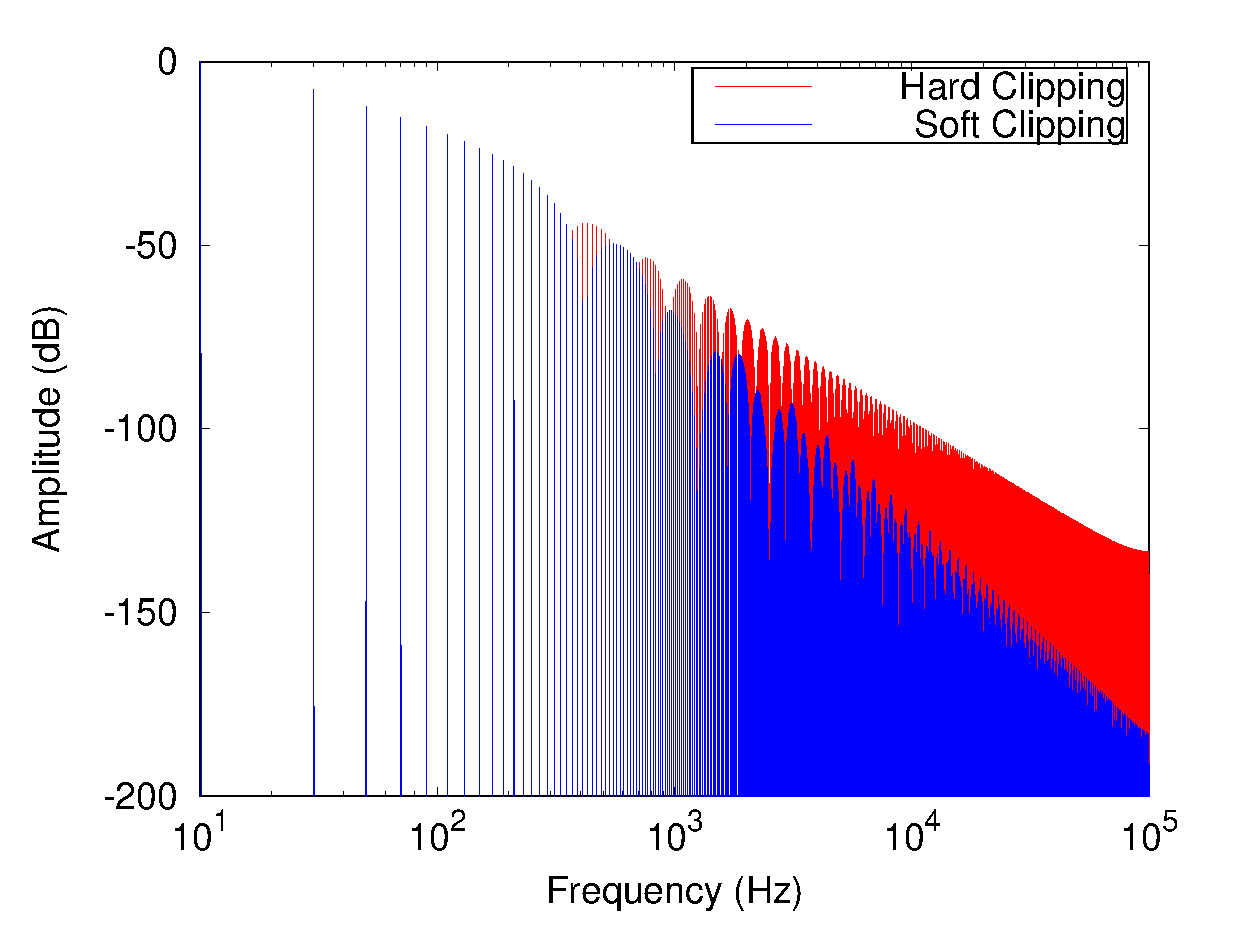
\includegraphics[width=0.6\textwidth]{chapter5/Images/ClippingSpectra.eps}
				\caption{Spectra of sinusoids clipped using Equations \ref{eq:SymmetricHardClipping} and
			                 \ref{eq:SymmetricSoftClipping}.}
				\label{fig:ClippingSpectra}
			\end{figure}

			The large amount of spectral content introduced by static nonlinearities means they are
			particularly susceptible to aliasing. Through smoothing the characteristic curve of the
			nonlinearity (making the clipper `softer') the amplitudes of generated frequencies will roll of
			more quickly. With lower levels of high order distortion the amplitudes of any aliased components
			will be reduced.

		\subsubsection*{Temporal Characteristics}
			As static nonlinearities are memoryless they can not influence the temporal evolution of signals at
			a large scale. There is a possibility to affect the attack and release times of signals slightly
			through increasing the gradient of the low amplitude section characteristic curve. As an extreme
			example consider the infinite peak clipper shown in Equation \ref{eq:InfinitePeakClipper}.

			\begin{equation}
				y[n] = \begin{cases}
					-1 & \text{if $x[n] < 0$} \\
					0 & \text{if $x[n] = 0$} \\
					1 & \text{if $x[n] > 1$}
				\end{cases}
				\label{eq:InfinitePeakClipper}
			\end{equation}
			
			Figure \ref{fig:InfinitePeakClipping} shows a signal, with attack and release sections, before and
			after infinite peak clipping. The original signal rises to its full amplitude over two cycles and
			falls back to silence over the same time. After infinite peak clipping the attack and release have
			become instantaneous.

			\begin{figure}[h!]
				\centering
				\includegraphics[width=0.6\textwidth]{chapter5/Images/InfinitePeakClipping.eps}
				\caption{A graph showing a signal before and after infinite peak clipping.}
				\label{fig:InfinitePeakClipping}
			\end{figure}

%		\subsubsection*{Flexibility}
%			For musical signals static nonlinearities introduce a spectrally rich band of audio. The spectral
%			content of which is highly dependent on that of the input signal. The bandwidth of the new set of
%			frequencies can be easily controlled through filtering or through the techniques discussed for
%			reducing aliasing. This allows for good performance in situations where energy needs to be added to
%			a specific area of the spectrum. 
			
%		\subsubsection*{Naturalness}

	\subsection{Rectification}
	\label{sec:ExcitationEvaluation-Methods-Rectification}
		Rectification is a special case of static nonlinearity. Signals can be either half or full wave rectified,
		as shown in Equations \ref{eq:HalfWaveRectification} and \ref{eq:FullWaveRectification} respectively.

		\begin{equation}
			y[n] = \begin{cases}
				0 & \text{if $x[n] < 0$} \\
				x[n] & \text{otherwise}
			\end{cases}
			\label{eq:HalfWaveRectification}
		\end{equation}

		\begin{equation}
			y[n] = \abs{x[n]}
			\label{eq:FullWaveRectification}
		\end{equation}

		\subsubsection*{Complexity}
			As with other static nonlinearities, rectifiers are very efficient. For full wave rectification
			only a single absolute value operation need be performed on each sample. Half wave rectification
			requires a comparison operation to detect negative samples before an assignment operation is
			applied.

		\subsubsection*{Homogeneity}
			One of the main advantages of rectifiers is that they are exhibit positive homogeneity (they
			satisfy Equation \ref{eq:homogeneity} only for non-negative values of $a$). For full wave
			rectification this can be summarised using Equation \ref{eq:FullWaveRectificationHomogeneity}.

			\begin{equation}
				\abs{ax[n]} = a\abs{x[n]}, \quad \forall a \in \textbf{R}_{\geq 0}
				\label{eq:FullWaveRectificationHomogeneity}
			\end{equation}

			Half wave rectification is not homogeneous for negative values of $a$ as the negative portions of
			the input signal are zeroed. If a negative gain is applied prior to this process, what were the
			positive portions of the input signal will be zeroed.

		\subsubsection*{Spectral Characteristics}
			Full wave rectification can be considered as a static nonlinearity with an even characteristics
			curve. As such it only introduces even order distortion components. The Fourier coefficients of a
			rectified sine wave are shown in Equation \ref{eq:RectificationFourier}.

			\[ c_{n} = \frac{1}{2\pi} \int_{-\pi}^{\pi} \abs{sin(x)}e^{-inx} dx \]

			\begin{equation}
				c_{n} = \begin{cases}
					\frac{2}{\pi(1 - n^{2})} & \text{when $n$ is even} \\
					0 & \text{when $n$ is odd}
				\end{cases}
				\label{eq:RectificationFourier}
			\end{equation}

			This represents all even order harmonics rolling off at approximately 12dB per octave.  As with
			other static nonlinearities rectifiers are susceptible to aliasing. The relatively shallow roll off
			of the distortion components can lead to a considerable amount of energy present in the aliased
			components of the output signal. 

			The output from a half wave rectifier has the same spectrum as that of a full wave rectifier
			but with the content of the original signal included. This can easily be shown by considering how a
			half wave rectified signal can be constructed from the original signal and a full wave rectified
			signal. Where $x(n)$, $x_{f}(n)$ and $x_{h}(n)$ represent the original signal, full wave rectified
			and half waves rectified signals respectively, their relationship can be seen in Equation
			\ref{eq:RectificationRelationship}.

			\begin{equation}
				x_{h}[n] = \frac{1}{2} \left( x_{f}[n] + x[n] \right)
				\label{eq:RectificationRelationship}
			\end{equation}

		\subsubsection*{Temporal Characteristics}
			Full wave rectifiers have no effect on the temporal characteristics of signals as all the magnitude
			of each sample is preserved. It is possible that a half wave rectifier could change the position of
			the onset of a signal by a small amount. Considering a signal which starts with a negative
			displacement. This first section of the signal would be removed, moving the onset to wherever the
			first positive displacement occurs.
			
%		\subsubsection*{Flexibility}
%			Rectifiers are useful when large amounts of even order distortion components are required. As with
%			other static nonlinearities the bandwidth of the newly introduced set of frequencies can be
%			controlled through filtering to provide more flexibility. 

%		\subsubsection*{Naturalness}

	\subsection{Integrator}
	\label{sec:ExcitationEvaluation-Methods-Integrator}
		Equation \ref{eq:Integrator} shows an Integrator adapted from the one described by \citet{larsen2004audio}.

		\begin{equation}
			y[n] = \begin{cases}
				0 & \text{if $x[n] > 0$ and $x[n - 1] \leq 0$} \\
				y[n - 1] + k\abs{x[n]} & \text{otherwise}
			\end{cases}
			\label{eq:Integrator}
		\end{equation}

		Where $k$ is the integration constant, effectively setting the output gain of the system. The output signal
		is reset to 0 ofter every negative to positive zero crossing in order to prevent the sample amplitudes from
		rising indefinitely.

		\subsubsection*{Complexity}
			For each sample two comparison operations are required to detect zero crossings. This is followed
			by some simple arithmetic operations in order to integrate the signal. While this may total more
			operations than a very basic static nonlinearity it still requires very little processing power.

			Unlike static nonlinearities the integrator shown in Equation \ref{eq:Integrator} requires memory
			to store the previous output sample. 

		\subsubsection*{Homogeneity}
			Integration is a homogeneous operation. This is an advantage over certain static nonlinearities as
			though more operations are needed per sample no further work is needed to make the system
			homogeneous. If a homogeneous system is required it may be more efficient to use an integrator over
			a static nonlinearity.
		
			\note
			{
				Formal proof?
			}

		\subsubsection*{Spectral Characteristics}
			Applying Equation \ref{eq:Integrator} to a sine wave produces a signal with Fourier coefficients as
			shown in Equation \ref{eq:IntegratorFourier}.

			\[ c_{n} = \frac{kf_{s}}{2\pi} \left( \int_{0}^{\pi} (1 - cos(x))e^{-inx} dx +
							       \int_{\pi}^{2\pi} (3 + cos(x))e^{-inx} dx \right) \]

			\[ c_{-1} = - \frac{2ikf_{s}}{\pi} \]
			\[ c_{0} = 2kf_{s} \]
			\[ c_{1} = \frac{2ikf_{s}}{\pi} \]
			\begin{equation}
				c_{n} = \frac{ikf_{s}}{2\pi} \left( \frac{4n^{2} + 2e^{-i\pi n} - 2}{n^{3} - n} \right)
				\label{eq:IntegratorFourier}
			\end{equation}

			This produces all harmonics with amplitudes rolling off at approximately 6dB per octave. This
			shallow roll of make integrators very useful when a large amount of new frequency content is
			desired. Due to the shallow roll of of the distortion component's amplitudes integrators are very
			prone to aliasing.

			While integrators are homogeneous they are frequency dependant acting as low pass filters. Using
			the same integration constant a high frequency input signal will produce a lower amplitude output
			than a low frequency input. This does not affect the relatives amplitudes of frequencies in the
			output just the overall amplitude of the signal.

		\subsubsection*{Temporal Characteristics}
			Due to the inherent low pass filtering behaviour of integrators the temporal properties of
			transient signals will be altered. Attacks times will be lengthened by the attenuation of their
			high frequency components. This prevents these methods being used where it is essential that
			transients are preserved. 
			
%		\subsubsection*{Flexibility}
%			Integrators provide an efficient means to add wideband energy to the spectrum of a signal. All
%			orders of distortion are generated making this new signal spectrally dense. The bandwidth of the
%			new signal can easily be controlled through filtering improving the flexibility.

%		\subsubsection*{Naturalness}

	\subsection{Multiplier}
	\label{sec:ExcitationEvaluation-Methods-Multiplier}
		Multipliers are a subset of static nonlinearities in which input samples are raised to a positive integer
		power as shown in Equation \ref{eq:Multiplier}.

		\begin{equation}
			y[n] = x[n]^{h}, \quad h \in \textbf{N}
			\label{eq:Multiplier}
		\end{equation}

		Exponential distortion extends this method by relaxing the restriction on the exponent ($h$), allowing it
		to take any positive value. The advantages and disadvantages of this will be discussed in this section.

		\subsubsection*{Complexity}
			Being a static nonlinearity the complexity of a multiplier is very low. A single exponentiation
			operation is applied to each sample. 

		\subsubsection*{Homogeneity}
			Exponentiation is a non-homogeneous operation. Any amplitude applied to a signal before processing
			is also raised to the exponent, as shown in Equation \ref{eq:MultiplierHomogeneity}.

			\begin{equation}
				(ax[n])^{h} = a^{h}x[n]^{h}
				\label{eq:MultiplierHomogeneity}
			\end{equation}

			Unlike clippers there is no threshold parameter to change in response to the amplitude of the input
			signal. Gain stages can be added before and after the nonlinearity in order to make the systems
			response to different input amplitudes more uniform.
			
		\subsubsection*{Spectral Characteristics}
			Nonlinear processing using Equation \ref{eq:Multiplier}, in which the exponent is a positive
			integer, allows for control over the maximum order of distortion generated. The highest frequency
			present among those generated will be equal to the highest frequency in the input signal multiplied
			by the exponent. This facilitates more control over the bandwidth of the generated signal providing
			greater flexibility and minimisation of aliasing.

			If the exponent is allowed to take any positive value, control over the bandwidth of the output
			signal is lost. Non integer exponents cause higher orders of distortion to be generated. Figures
			\ref{fig:CubedSpectra} and \ref{fig:TwoAndAHalfSpectra} show the spectral effects of exponential
			distortion with integer and non integer exponents. The input signal has a fundamental frequency of
			1kHz and has energy in the first four harmonics.

			\begin{figure}[h!]
				\centering
				\includegraphics[width=0.6\textwidth]{chapter5/Images/CubedSpectra.eps}
				\caption{The spectral effects of cubing a signal with energy in its first four harmonics.}
				\label{fig:CubedSpectra}
			\end{figure}

			\begin{figure}[h!]
				\centering
				\includegraphics[width=0.6\textwidth]{chapter5/Images/RaisedToTwoAndAHalfSpectra.eps}
				\caption{The spectral effects of raising a signal with energy in its first four harmonics
					 to the power 2.5.}
				\label{fig:TwoAndAHalfSpectra}
			\end{figure}

			The highest frequency component in the original signal is 4kHz. After cubing the signal the highest
			frequency is three times this (12kHz) as seen in Figure \ref{fig:CubedSpectra}. Figure
			\ref{fig:TwoAndAHalfSpectra} shows that when the exponent is 2.5 higher frequency components are
			introduced. 

		\subsubsection*{Temporal Characteristics}
			Exponential distortion has a dynamic compression/expansion effect. For exponents greater than 1 the
			dynamics of a signal are expanded, the amplitude difference between low and high amplitude portions
			of the signal is increased. For exponents less that 1 the opposite occurs, compressing the dynamics
			of the signal. Figure \ref{fig:ExponentiationTemporalEffects} show the effects this can have on the
			attack and release portions of signals.

			\begin{figure}[h!]
				\centering
				\includegraphics[width=0.6\textwidth]{chapter5/Images/ExponentiationTemporalEffects.eps}
				\caption{The temporal effects of exponential distortion.}
				\label{fig:ExponentiationTemporalEffects}
			\end{figure}

			While the time taken for the signal to rise to or decay from maximum amplitude is not changed, the
			shape of the amplitude envelope during the attack and release portions is. 

		\subsubsection*{Flexibility}
			Multipliers offer greater flexibility than the previously discussed excitation methods. Control
			over the orders of distortion introduced allows for finer shaping of a signals spectrum. The output
			of several multipliers with different exponents can be summed in order to include multiple orders
			of distortion.

			Summing multiplier outputs in this way allows for approximation of other static
			nonlinearities. A low order polynomial expression approximating the desired characteristic curve
			is calculated by linear regression as shown in Figure \ref{fig:ClippingApproximation}. The
			order of the polynomial controls the maximum order of the distortion components.

			\begin{figure}[h!]
				\centering
				\includegraphics[width=0.6\textwidth]{chapter5/Images/ClippingApproximation.eps}
				\caption{A 7\super{th} order approximation of hard clipping using linear regression.}
				\label{fig:ClippingApproximation}
			\end{figure}

			Generating characteristic curves in this way reduces the number of aliased frequencies at the cost
			of having to evaluate a more complex polynomial to calculate the output value for each sample. A
			similar approach is undertaken by \cite{fernandez-cid2001distortion} who construct characteristic
			curves from Chebyshev polynomials in order to control the highest frequencies introduced.

%		\subsubsection*{Naturalness}

	\subsection{Single Side Band Automodulation}
	\label{sec:ExcitationEvaluation-Methods-SSBA}
		Single sideband automodulation (SSBA) utilises the concept of single sideband modulation
		\citep{corinthios2009signals}. This allows you to apply amplitude modulation to a signal and only produce
		either the sum or difference sideband.

		A simple way to apply single sideband modulation to a signal is through construction of an analytic signal.
		An analytic signal is a complex valued signal, the real part of which is the original signal and the
		imaginary part its Hilbert transform. The analytic signal is often denoted with a subscript letter
		$a$, such that the analytic representation of the signal $x(n)$ would be denoted $x_{a}(n)$.

		An ideal Hilbert transform alters the phase information of a signal while leaving the magnitude information
		unchanged. Any negative frequencies in the signal have their phase shifted by $\frac{\pi}{2}$ radians.  The
		phase of positive frequencies is shifted by $-\frac{\pi}{2}$ radians. The transfer function for an FIR
		implementation of a Hilbert transform is shown in Equation \ref{eq:FirHilbertTransform}.

		\begin{equation}
			H(z) = \sum_{m = -M}^{M} \frac{2}{m\pi} sin^{2} \left( \frac{m\pi}{2} \right) z^{-m}
			\label{eq:FirHilbertTransform}
		\end{equation}

		For an ideal Hilbert transform the impulse response should be infinitely long ($M = \infty$). Practicable
		approximations of an ideal Hilbert transform can be created by using a finite value for $M$. A delay of $M$
		samples must also be introduced in order to make the filter causal. As the value of $M$ is decreased this
		delay is reduced while the magnitude response of the filter deviates further from the ideal. Figure
		\ref{fig:HilbertMagnitude} shows the magnitude responses for FIR Hilbert transform filters with $M = 11$
		and $M = 101$. The filters have a bandpass response with some ripple in the pass band. As $M$ is increased
		the bandwidth of the passband is increased and the ripple reduced. The phase response of these filters
		remains ideal no matter the value of $M$, as evidenced by Figure \ref{fig:HilbertPhase}.

		\begin{figure}[h!]
			\centering
			\includegraphics[width=0.6\textwidth]{chapter5/Images/HilbertMagnitudeResponses.eps}
			\caption{Magnitude responses of FIR Hilbert transform filter with different orders.}
			\label{fig:HilbertMagnitude}
		\end{figure}

		\begin{figure}[h!]
			\centering
			\includegraphics[width=0.6\textwidth]{chapter5/Images/HilbertPhaseResponses.eps}
			\caption{Phase responses of FIR Hilbert transform filters with different orders.}
			\label{fig:HilbertPhase}
		\end{figure}

		When using Equation \ref{eq:FirHilbertTransform} a compromise needs to be made between the tolerable amount
		of delay and the accuracy of the filter's magnitude response. Increasing $M$ will give a more accurate
		filter but introduce more delay and increase the complexity of the filter. More efficient implementations
		can be build using IIR filters if some of the properties of an ideal Hilbert transform are disregarded.

		\citet{oppenheim2014discrete} suggest constructing a phase splitter: processing audio with two parallel
		allpass IIR filters the phase responses of which differ from each other by $\frac{\pi}{2}$ radians for a
		large proportion of the spectrum. While this is not strictly a Hilbert transform it creates two signals
		which can be used as the real and imaginary part of an analytic signal. \citet{niemitalo2003hilbert}
		provides an implementation of such a pair of filters. The phase difference between these two filters is
		seen in Figure \ref{fig:IIRHilbertPhase}.

		\begin{figure}[h!]
			\centering
			\includegraphics[width=0.6\textwidth]{chapter5/Images/IIRHilbertPhaseResponses.eps}
			\caption{The phase difference between the two allpass filters proposed by
			         \citet{niemitalo2003hilbert}.}
			\label{fig:IIRHilbertPhase}
		\end{figure}

		In single sideband automodulation the analytical representation of the input signal is multiplied with
		itself in order to generate harmonics. Equation \ref{eq:SSB} shows the $h$\super{th} order single side
		band automodulation of a signal.

		\begin{equation}
			y[n] = \Re \left( x_{a}[n]^{h} \right), \quad h \in \textbf{N}
			\label{eq:SSB}
		\end{equation}

		\subsubsection*{Complexity}
			Compared with the harmonic excitation methods discussed previously, single sideband automodulation
			has greater complexity. A Hilbert transform must be applied before a complex exponentiation
			operation for each sample. The Hilbert transform filter used must give similar response for a wide
			range of frequencies so the resulting harmonic excitation gives similar results at different
			frequencies.
			
			A high order FIR Hilbert transform filter is required to give a suitably flat magnitude response.
			A lower complexity IIR phase splitter can be used in order to reduce the computational load.
			The implementations given by \citet{niemitalo2003hilbert} consists of eight biquad filters and a
			one sample delay.
			
		\subsubsection*{Homogeneity}
			As with multipliers, SSBA is a non-homogeneous process. The amplitude envelope of the $h$\super{th}
			order automodulation is the amplitude envelope of the original signal raised to the power $h$. 

			\note
			{
				Formal proof?
			}

		\subsubsection*{Spectral Characteristics}
			SSBA extends the control provided by multipliers as it constrains the minimum frequency introduced
			as well as the highest. Using Equation \ref{eq:SSB} only the upper sideband (the sum frequencies)
			of the modulation is produced. The highest and lowest frequency components of the output are that
			of the input signal multiplied by the exponent. Between these two frequencies lie all the other
			harmonic and intermodulation components created. This can be seen in figure \ref{fig:SSBA3Spectra},
			which shows the results of applying $3^{rd}$ order SSBA to the signal used in Figures
			\ref{fig:CubedSpectra} and \ref{fig:TwoAndAHalfSpectra}. 			
			
			\begin{figure}[h!]
				\centering
				\includegraphics[width=0.6\textwidth]{chapter5/Images/SSBA3Spectra.eps}
				\caption{The spectral effects of applying third order SSBA to a signal with energy in its 
				         first four harmonics.}
				\label{fig:SSBA3Spectra}
			\end{figure}

			If aliasing does occur it is possible for the aliased frequency to lie outside of this bandwidth.
			The amplitude of aliased frequencies can be greatly reduced through filtering. Applying a low pass
			filter with a cutoff frequency of $\frac{f_{s}}{2h}$ prior to processing will reduce the amplitude
			of any frequency content in the input which will cause aliasing when processed.

		\subsubsection*{Temporal Characteristics}
			SSBA has similar temporal effects to a multiplier using an exponent greater that 1. The signal
			undergoes dynamic expansion changing the shape of its attack and release envelopes as shown in
			Figure \ref{fig:SSBATemporalEffects}.

			\begin{figure}[h!]
				\centering
				\includegraphics[width=0.6\textwidth]{chapter5/Images/SSBATemporalEffects.eps}
				\caption{The temporal effects of SSBA.}
				\label{fig:SSBATemporalEffects}
			\end{figure}

			The restricted bandwidth of the SSBA technique's output is also apparent from this graph. The input
			is a sinusoid with a simple amplitude envelope. The output is a sinusoid with 3 times the frequency
			and an amplitude envelope equal to that of the input cubed. This is in contrast to the effect of
			the multiplier shown in Figure \ref{fig:ExponentiationTemporalEffects} where the output signal is
			no longer sinusoidal.

%		\subsubsection*{Flexibility}
%		\subsubsection*{Naturalness}

	\subsection{Instantaneous Amplitude and Phase}
	\label{sec:ExcitationEvaluation-Methods-IAP}
		In this method, the instantaneous amplitude and phase (IAP) of the analytic signal are calculated. These
		values are then used to aid in the construction of harmonics. The instantaneous amplitude of the analytic
		signal is found by taking its absolute value, $\abs{x_{a}[n]}$. The instantaneous phase is found by taking
		the complex argument of the analytic signal, $\arg(x_{a}[n])$. The instantaneous phase can then be scaled
		in order to scale the frequency content of the signal independent of its amplitude. Equation \ref{eq:IAP}
		shows the $h$\super{th} order instantaneous amplitude and phase modulation of a signal.

		\begin{equation}
			y[n] = \abs{x_{a}[n]} \cos \left( h\arg(x_{a}[n]) \right), \quad h \in \textbf{N}
			\label{eq:IAP}
		\end{equation}

		\subsubsection*{Complexity}
			The IAP technique requires a Hilbert transform to be performed before the harmonic generation. The
			computational load of this is the same as that for the SSBA technique, an IIR phase splitter
			implementation providing a good compromise between accuracy, complexity and delay. Once an analytic
			signal has been constructed the remaining processing is applied on a sample by sample basis. 
			
		\subsubsection*{Homogeneity}
			In the IAP method the magnitude and phase information of a signal are separated. The phase
			information is scaled in order to increase the frequency while the magnitude information is left
			unaltered. This preservation of magnitude information mean that the IAP method is a homogeneous
			system.

			\note
			{
				Formal proof?
			}
			
		\subsubsection*{Spectral Characteristics}
			In contrast to the SSBA method, the IAP method is homogeneous but provides little control over the
			bandwidth of the output when the input has multiple frequency components. Figure
			\ref{fig:IAP3Spectra} shows the spectral effects of third order IAP processing on the same signal
			used when discussing previous algorithms.

			\begin{figure}[h!]
				\centering
				\includegraphics[width=0.6\textwidth]{chapter5/Images/IAP3Spectra.eps}
				\caption{The spectral effects of applying third order IAP to a signal with energy in its 
				         first four harmonics.}
				\label{fig:IAP3Spectra}
			\end{figure}

			When multiple frequency components are present in the input signal IAP processing produces energy
			at high order distortion components. As with previous algorithms it may be necessary to upsample
			the signal before precessing to avoid aliasing of these frequencies.

		\subsubsection*{Temporal Characteristics}
			The homogeneity of the system preserves the input signals amplitude envelope. Due to this the
			temporal characteristics of signals are unaffected. This can be seen in Figure
			\ref{fig:IAPTemporalEffects}, it is apparent that the frequency of the sinusoid has been altered
			and its amplitude envelope not.

			\begin{figure}[h!]
				\centering
				\includegraphics[width=0.6\textwidth]{chapter5/Images/IAPTemporalEffects.eps}
				\caption{The temporal effects of IAP.}
				\label{fig:IAPTemporalEffects}
			\end{figure}
			
%		\subsubsection*{Flexibility}
%		\subsubsection*{Naturalness}

	\subsection{Spectral Replication}
	\label{sec:ExcitationEvaluation-Methods-SpectralReplication}
		The principle behind spectral replication is to reproduce the spectral structure of a signal at higher
		frequencies as shown in Figure \ref{fig:SpectralReplication}.

		\begin{figure}[h!]
			\centering
			\includegraphics[width=0.6\textwidth]{chapter5/Images/SpectralReplicationSpectrum.eps}
			\caption{Reproduction of a signal at higher frequencies.}
			\label{fig:SpectralReplication}
		\end{figure}

		This spectral shift is easily implemented through the use of single sideband modulation with a complex
		sinusoid as shown in Equation \ref{eq:SpectralReplication}.

		\begin{equation}
			y[n] = \Re \left( x_{a}[n] e^{2i\pi fn/ f_{s}} \right)
			\label{eq:SpectralReplication}
		\end{equation}

		Where $f$ is the amount by which the signals spectrum should be shifted.

		\subsubsection*{Complexity}
			Again, this method requires a Hilbert transform of the signal to be taken adding to the overall
			complexity of the system. After this the synthesis of a complex sinusoid needs to be carried out
			followed by the multiplication of the two complex signals on a sample by sample basis.

		\subsubsection*{Homogeneity}
			Spectral replication using Equation \ref{eq:SpectralReplication} is a homogeneous process.

			\note
			{
				Formal proof?
			}
			
		\subsubsection*{Spectral Characteristics}
			In spectral replication each frequency component is shifted by the same amount preserving the size
			of the spacings between them. This is useful for harmonic excitation of simple harmonically
			structured signals. Providing the spectrum is shifted by an integer multiple of the fundamental
			frequency any components at harmonic frequencies in the input will remain harmonic frequencies at
			the output. This process avoids the intermodulation distortion inherent to the systems discussed
			previously. 

			Due to every frequency component being shifted by an equal amount the bandwidth of the output is
			equal to that of the input. This predictability allows for easier control of the output spectrum.
			It also provides a simple method for reduction of aliasing. The highest frequency in the output
			will be that of the input plus the sift frequency $f$. Applying a low pass filter, with a cutoff
			frequency of $f_{s} - f$Hz to the input will help minimise the amplitude of any aliased
			frequency components.

		\subsubsection*{Temporal Characteristics}
			Spectral replication does not affect the temporal properties of a signal.

%		\subsubsection*{Flexibility}
%		\subsubsection*{Naturalness}

	\subsection{Spectral Folding}
	\label{sec:ExcitationEvaluation-Methods-SpectralFolding}
		Spectral folding uses upsampling in order to replicate parts of the spectrum at higher frequencies. In
		order for the output signal to have the same sampling frequency as the input the signal is 
		downsampled by a factor $k$ before being upsampled by the same factor. 
		
		To avoid aliasing during the downsampling phase the signal should have a low pass filter applied
		with a cutoff frequency of $\frac{f_{s}}{2k}$. Typically upsampling systems apply a low pass filter
		to remove any high frequency content introduced \citep{oppenheim2014discrete}. This is not needed for
		spectral folding as the production of high frequency energy is the desired result.

		After filtering, the downsampling and upsampling can be performed at the same time by retaining
		every $k$\super{th} sample and setting all others to zero. This is shown in Equation
		\ref{eq:SpectralFolding} where $x_{lf}[n]$ is the filtered input signal.		

		\begin{equation}
			y[n] = \begin{cases}
				x_{lf}[n] & \text{if $k \divides n$} \\
				0 & \text{otherwise}
			\end{cases}
			\label{eq:SpectralFolding}
		\end{equation}

		\subsubsection*{Complexity}
			Spectral folding using Equation \ref{eq:SpectralFolding} is relatively simple requiring only a low
			pass filter and some additional assignment operations. The complexity of the system as a whole
			largely depends on the complexity of the downsampling filter used.

		\subsubsection*{Homogeneity}
			Both downsampling and upsampling are homogeneous processes making spectral folding also
			homogeneous.

			\note
			{
				Formal proof?
			}
			
		\subsubsection*{Spectral Characteristics}
			Spectral folding with a factor $k$ results in the lowest $\frac{1}{k}$ of the input spectrum being
			repeated $k$ times in the output spectrum. Every second repetition is a mirror image of the
			original. This effect is shown in Figure \ref{fig:SpectralFolding}. 
			
			\begin{figure}[h!]
				\centering
				\includegraphics[width=0.6\textwidth]{chapter5/Images/SpectralFoldingSpectrum.eps}
				\caption{The spectral characteristics of spectral folding.}
				\label{fig:SpectralFolding}
			\end{figure}

			The new frequencies introduced in the output depend on the sampling rate of the signal. Unless
			$\frac{f_{s}}{2k}$ is a harmonic of the input signal there is little chance that the new
			frequencies will be harmonically related to the input.

			Other than changing the downsampling / upsampling factor, the user is given little control over the
			content of the output spectrum. The bandwidth of the output is not constricted, possibly taking up
			the entirety of the spectrum. Additional filtering is needed to shape the output spectrum as
			desired, increasing the overall complexity of the system.

		\subsubsection*{Temporal Characteristics}
			The low pass filter applied as part of the downsampling phase removes the high frequency content
			which contributes to transients in the signal. This has the effect of lengthening attack times
			similar to the effect seen in the Integrator system (Section
			\ref{sec:ExcitationEvaluation-Methods-Integrator}).

		\subsubsection*{Flexibility}
			Spectral folding is an efficient method by which to create a dense output spectrum but has many
			downsides.

%		\subsubsection*{Naturalness}

	\subsection{Spectral Stretching}
	\label{sec:ExcitationEvaluation-Methods-SpectralStretching}
		The principle of spectral stretching is to scale the spectrum of a signal along the frequency axis. This
		effect is shown in Figure \ref{fig:SpectralStretching}.

		\begin{figure}[h!]
			\centering
			\includegraphics[width=0.6\textwidth]{chapter5/Images/SpectralStretchingSpectrum.eps}
			\caption{The spectral characteristics of spectral stretching.}
			\label{fig:SpectralStretching}
		\end{figure}

		A typical implementation of this effect utilises a phase vocoder. The phase vocoder is an algorithm which
		allows for time stretching of a signal. It is applied by calculating the short-time Fourier transform of a
		signal with a given frame and hop size. The signal is then resynthesised using a different hop size in
		order to either lengthen or shorten it. This signal can then be resampled back to the length of the
		original signal scaling the frequency content in the process. 
		
		The spectrum is scaled by a factor given in Equation \ref{eq:PhaseVocoderFactor}.

		\begin{equation}
			s = \frac{h_{s}}{h_{a}}
			\label{eq:PhaseVocoderFactor}
		\end{equation}

		Where $h_{a}$ is the hop size used when calculating the STFT and $h_{s}$ is the hop size used to
		resynthesise the signal.
		
		\subsubsection*{Complexity}
			Spectral stretching using a phase vocoder require are large amount of computation. Calculating the
			STFT involves splitting the signal into frames of which the DFT is then computed. The phase
			correction for each frame must then be computed and applied before the inverse DFT of each frame is
			taken and the frames summed back together. The resulting signal then needs to be resampled
			requiring further operations. If the scaling factor is not an integer value the resampling process
			will require additional interpolation calculations.
		
			Several steps can be taken to reduce the work needed when using a phase vocoder. The computational
			complexity of the DFT calculations can be reduced by using the fast Fourier transform
			\citep{portnoff1976implementation}. When shifting the frequencies upwards the amount of work can be
			further reduced by resampling the signal before calculating the STFT \citep{laroche1999new}. This
			way there are less frames for which the DFT need be calculated.
			
		\subsubsection*{Homogeneity}
			The phase vocoder algorithm is a homogeneous system. When processing the signal in the frequency
			domain only the phase information is altered, leaving magnitude information unchanged. 

			\note
			{
				Formal proof?
			}

		\subsubsection*{Spectral Characteristics}
			An ideal spectral stretching system would produce the result shown in Figure
			\ref{fig:SpectralStretching}. All frequency components are scaled by the same factor. For
			harmonically structured signals this has the effect of scaling the fundamental frequency.

			The phase vocoder introduces some artefacts during its operation. The process of splitting the
			signal into frames causes spectral leakage. Energy at a given frequency is spread across the nearby
			frequencies. In a signal which only has energy at harmonic frequencies, spectral stretching by an
			integer factor will produce some inharmonic content due to this effect. Spectral leakage can be
			minimised through the use of windowing functions such as the Hamming or Blackman-Harris windows. 

			Ignoring the effect of spectral leakage, the bandwidth of the output signal will be that of the
			input multiplied by the stretching factor. This allows for effective minimisation of aliasing as
			the signal can be low pass filtered before processing as done with single sideband automodulation
			(Section \ref{sec:ExcitationEvaluation-Methods-SSBA}).
		
		\subsubsection*{Temporal Characteristics}
			A simple phase vocoder implementation produces artefacts when processing transients in a signal.
			The phase correction stage before resynthesis can have the effect of softening the attack portion.
			The exact effect had on the transient is not able to be controlled as it depends on where the
			transient lies in the STFT frame. \citet{robel2003a} proposes a method to better process transients
			with a phase vocoder. An algorithm is used to detect the presence of transients in an STFT frame.
			The phase information is then processed differently depending on the position of the transient
			within the frame.

%		\subsubsection*{Flexibility}
%		\subsubsection*{Naturalness}

	\subsection{Short-Time Time Reversal}
	\label{sec:ExcitationEvaluation-Methods-STTR}
		Short-Time time reversal (STTR) is an audio effect proposed by \citet{kim2014shorttime}. The output signal
		is constructed from overlapping frames of the input signal which have been reversed in time using Equation
		\ref{eq:STTR}.

		\begin{equation}
			y[n] = \sum_{m = -\infty}^{\infty} w[n - mR]x[2mR - n]
			\label{eq:STTR}
		\end{equation}

		Where $R$ is the step size in samples and $w$ is some window function with constant overlap add (i.e. the
		sum of the window function translated in time by all integer multiples $R$ is one for all values of $n$
		(Equation \ref{eq:ConstantOverlapAdd})).

		\begin{equation}
			\sum_{m = -\infty}^{\infty} w[n - mR] = 1
			\label{eq:ConstantOverlapAdd}
		\end{equation}

		Constant overlap add ensures that no unwanted amplitude modulation is applied to the signal.

		\subsubsection*{Complexity}
			The computational complexity of STTR depends on the ratio of the step size, $R$, and the length of
			the window function $L$ in samples. As $\frac{R}{L}$ decreases the number of overlapping frames
			needed to calculate an output sample increases, increasing the computational load.

			Time reversal of the frames introduces an $L$ sample delay to the signal as the samples at the end
			of the first frame are needed to form the start of the signal.
			
		\subsubsection*{Homogeneity}
			STTR is a homogeneous process. As the samples in each frame are only multiplied
			by a constant window and reversed in time non of the amplitude information in the signal is lost. 

			\note
			{
				Formal proof?
			}

		\subsubsection*{Spectral Characteristics}
			The spectral effects of STTR depend on factors of the input signal and the window function and
			step size used. For simple sinusoidal inputs complex output spectra can be generated. For example
			consider the spectral effects of STTR using the window function defined in Equation
			\ref{eq:STTRWindow} (shown in Figure \ref{fig:STTRWindow}).

			\begin{equation}
				w[n] = \begin{cases}
					\cos \left( \frac{4\pi n}{3L} \right) & \text{if $\abs{n} \leq \frac{L}{4} $} \\
					1 - \cos \left( 2\pi \frac{2n - \sgn(n)L}{3L} \right) &
						\text{if $\frac{L}{4} < \abs{n} \leq \frac{L}{2}$} \\
					0 & \text{otherwise}
				\end{cases}
				\label{eq:STTRWindow}
			\end{equation}

			\begin{figure}[h!]
				\centering
				\includegraphics[width=0.6\textwidth]{chapter5/Images/STTRWindow.eps}
				\caption{The window function defined in Equation \ref{eq:STTRWindow}.}
				\label{fig:STTRWindow}
			\end{figure}

			This window function exhibits constant overlap add for a step size of $\frac{L}{2}$.

			Figure \ref{fig:STTRSpectra} shows the output spectra of STTR, using this window with lengths of
			1ms and 1.5ms, on a 1kHz sinusoid.

			\begin{figure}[h!]
				\centering
				\includegraphics[width=0.6\textwidth]{chapter5/Images/STTRSpectra.eps}
				\caption{The spectral effects of STTR using the window function defined in Equation
				         \ref{eq:STTRWindow}.}
				\label{fig:STTRSpectra}
			\end{figure}

			The complexity of the output spectrum depends on the relationship of the input frequency and the
			step size used for processing. If the period of the input signal is an integer multiple of the step
			size it will remain unchanged by the processing. This is evidenced by the output spectrum for 1ms
			window shown in Figure \ref{fig:STTRSpectra}, only odd order harmonics are generated retaining the
			original period of the signal.

			The period of the output signal is the least common multiple of the period of the input signal and
			the step size. This causes the period of a signal to be increased when the period of the input is
			not an integer multiple of the step size. The output spectrum for a 1.5ms window shows this. The
			period of the output becomes 3ms. The lowest frequency in this output is then approximately 333Hz.

			The exact frequencies of the partials in the output are discussed by \citet{kim2014shorttime}. In
			effect they are the intermodulation frequencies of the input frequency and the step frequency (1
			over the step size in seconds). The amplitudes of these partials are influenced by the Fourier
			transform of the window function used. This allows the spectral characteristics of the output to be
			loosely controlled through manipulation of the window function and step size.

			There is no upper bound on the frequency of the output so upsampling may need to be use to minimise
			aliasing.

		\subsubsection*{Temporal Characteristics}
			Due to the time reversal STTR can have complicated effects on a signals amplitude envelope.
			For instance, the attack and release portion of a sound may be switched. While possible, this is
			highly dependent on the window length, step size and content of the input frequency. Controlling
			these aspect for general input signals proves a very difficult task.

		\subsubsection*{Flexibility}
			STTR can be used, much like a static nonlinearity, as a method of generating wide bands of
			high order harmonics. Unlike static nonlinearities however it is possible to generate inharmonic
			partials for a sinusoidal input. The generation of theses is dependant on properties of the input
			signal adding further complexity to predicting the effects for arbitrary input signals.

			\citet{kim2015harmonizing} suggest methods through which the output of STTR can be controlled in
			the implementation of a harmonising effect. This effect introduces new tones, at different
			musical intervals, depending on the input frequency. While this is useful as a compositional tool
			it does not provide the uniform response across input signals required for timbral control.

\begin{landscape}
\section{Methods Comparison}
\label{sec:ExcitationEvaluation-Comparison}

	\begin{tabular}{|c|c|c|c|c|c|c|}
		\hline
		\bf{Method} & \bf{Complexity} & \bf{Homogeneity} & \bf{Spectral Properties} & \bf{Temporal Properties} &
		\bf{IMD} & \bf{Flexibility} \\ % & \bf{Naturalness} \\
		\hline
		Static Nonlinearity & $\mathcal{O}(n)$ & & & & & \\
		\hline
		Rectifier & $\mathcal{O}(n)$ & & & & & \\
		\hline
		Integrator & $\mathcal{O}(n)$ & & & & & \\
		\hline
		Multiplier & $\mathcal{O}(n)$ & & & & & \\
		\hline
		SSBA & $\mathcal{O}(n)$ & & & & & \\
		\hline
		IAP & $\mathcal{O}(n)$ & & & & & \\
		\hline
		Spectral Replicator & $\mathcal{O}(n)$ & & & & & \\
		\hline
		Spectral Mirror & $\mathcal{O}(n)$ & & & & & \\
		\hline
		Spectral Stretch & $\mathcal{O}(n\log{n})$ Assuming FFT used & & & & & \\
		\hline
	\end{tabular}

\end{landscape}

\section{Key Findings}
	\note
	{
		Conclude the chapter.
	}

%\section{Evaluating Excitation Methods}
%\label{sec:FeatureControl-MethodEvaluation}
%
%	\note{Homogeneity a la DAFx paper.
%	      Flexibility introduced by allowing single harmonic control a la SMC paper}
%
%	Several harmonic excitation methods were discussed in Section \ref{sec:ExcitationEvaluation-Methods}. When applied to the 
%	task of controlling specific audio features each of these methods has its own advantages and disadvantages.
%
%	\subsection{Homogeneity}
%	\label{sec:FeatureControl-Homogeneity}
%
%		\subsubsection*{Static Nonlinearities}		
%			As previously mentioned simple static nonlinearities are very susceptible to change in input 
%			amplitude. \citet{deman2014adaptive} counteract this issue by having the clipping threshold adapt 
%			to changes in the RMS amplitude of the input. The user is then provided with a `relative threshold' 
%			parameter on which the same setting should give similar perceptual results no matter what the input 
%			amplitude.
%
%			\note{Talk about the issues with static nonlinearities raised in \citet{enderby2012harmonic}}
%
%		\subsubsection*{Bandwidth Extension}
%			\note{Spectral mirroring, stretching and replication are all homogeneous.}
%			
%		\subsubsection*{Single Harmonic Generation}
%			Using single sideband automodulation the proportion of new frequency components in the output 
%			signal increases as the input amplitude increases. The instantaneous amplitude and phase and phase 
%			vocoder techniques are more robust in this respect.
%
%	\subsection{Flexibility}
%	\label{sec:FeatureControl-Flexibility}
%
%		\note{Flexibility is provided by individual harmonic generation \citep{enderby2013methods}}	
%
%	\subsection{Complexity}
%	\label{sec:FeatureControl-Complexity}
%		
%		\note{It is advantageous to use an algorithm that will create accurate harmonics with little analysis.
%		      Most methods don't rely on knowing the fundamental in order to generate harmonics. Spectral
%		      shifting on the other hand does.}
%
%		\note{Most of the algorithms can be easily improved through the use of a low pass filter, increasing
%	             complexity.}

%Suitability of Exciters for Perceptual Control
%	Parameterise feature changes in terms of harmonic excitation.
%	Most suitable methods for given feature manipulations.
%	Easiest features to control in isolation.

\chapter{Controlling Audio Features} % control of low level features using exciters
\label{chap:FeatureControl}

\section{Introduction}
\label{sec:FeatureControl-Introduction}
	Previous studies, discussed in Section~\ref{sec:Timbre-Control}, have attempted to control perceptual features
	(such as warmth and brightness) by controlling specific audio features. The characteristics of the harmonic
	excitation systems discussed in Chapter~\ref{chap:ExcitationEvaluation} can be utilised to provide similar control
	over audio features. Ideally, control over a feature should be linear (the relationship between the effect's
	parameter setting the feature value being linear) and independent (the effect only controls one audio feature, the
	rest remaining constant). This would allow for the most flexibility in applying timbral transforms, every separate
	feature can be set individually and predictably. In reality this is not achievable: providing linear control
	requires in depth analysis of the input signal which cannot be applied in real time. In addition, independent
	control of features is not always possible as several features are closely related, such as spectral flatness and
	spectral irregularity. In light of this, the techniques developed in this chapter will focus on providing monotonic
	control over an audio feature: a given direction in change of parameter setting will always produce the same
	direction of change of the audio feature.
	
	This chapter will provide methods by which selected audio features can be controlled through harmonic excitation
	and determine which excitation algorithms are the most suitable for given feature changes. Firstly, in
	Section~\ref{sec:FeatureControl-Systems}, various challenges which arise when building harmonic excitation systems
	are discussed and methods to counteract them are suggested. A number of different systems are proposed which
	provide control over the nature of the new frequency components introduced to the signal. In
	Section~\ref{sec:FeatureControl-Parameterisation} methods by which these systems can be configured to provide
	monotonic control over specific audio features are proposed and tested.

\section{Harmonic Excitation Systems}
\label{sec:FeatureControl-Systems}
	In Section~\ref{sec:Excitation-Methods}, several different methods of introducing new frequency content to a signal
	were introduced. In Section~\ref{sec:ExcitationEvaluation-Comparison} these methods were discussed further and the
	degree to which their effects can be controlled was evaluated. From that analysis it is known that better control
	over the output is gained through meeting certain input requirements, for instance the \acrshort{ssba} and
	\acrshort{iap} techniques will produce sinusoidal outputs for sinusoidal inputs. It is also noted that further
	filtering may be needed alongside the use of a harmonic excitation algorithm in order to shape the spectrum as
	desired. Harmonic excitation systems can be constructed which apply this pre and post-processing before and after a
	given harmonic excitation algorithm. This section discusses the design of these systems, aiming to give users
	precise control over the new spectral content added to a wide range of input signals.

	\subsection{$f_{0}$ Tracking}
	\label{sec:FeatureControl-Systems-Fundamental}
		As discussed in Section~\ref{sec:ExcitationEvaluation-Comparison}, the behaviour of several of the harmonic
		excitation systems is more predictable for sinusoidal inputs. This is due to the elimination of
		intermodulation distortion components by having an input signal consisting of only a single frequency. This
		more predictable behaviour simplifies the problem of using harmonic excitation algorithms in providing
		monotonic control of audio features, allowing similar transforms to be applied to a wide range of input
		signals. To take advantage of this improvement in predictability, the input signal to a harmonic exciter
		must be pre-processed such that it is represented by a single sinusoid. For monophonic, tonal sources, this
		can be achieved by representing this signal as a sinusoid at the input's $f_{0}$. The remainder of this
		thesis then focusses on controlling timbre in this class of audio signal. Other classes of signal
		(polyphonic, noisy etc.) are left for consideration in future work.
		
		A monophonic, tonal signal can be represented as a sinusoid by applying a band pass filter centered around
		its $f_{0}$. This produces a narrowband signal with the majority of its energy concentrated at the $f_{0}$.
		In the following discussion this filtered signal will be referred to as the `isolated $f_{0}$'. Applying a
		harmonic excitation algorithm to the isolated $f_{0}$ will produce a signal with lower levels of
		intermodulation components than processing the original input signal. The `excited' isolated $f_{0}$ signal
		can then be summed with the original signal to produce the output. A diagram of this system is shown in
		Figure~\ref{fig:F0Tracking}.

		\begin{figure}[h!]
			\centering
			\begin{tikzpicture}
				\node (In) at (0, 1) {$x[n]$};
				\coordinate (InMid) at (1, 1);
				\draw (In) -- (InMid);

				\coordinate (Through) at (1, 0);
				\draw (InMid) -- (Through);
				\coordinate (ThroughOut) at (9, 0);
				\draw (Through) -- (ThroughOut);

				\coordinate (Side) at (1, 2);
				\draw (InMid) -- (Side);

				\node (F0) [draw] at (2.5, 2) {$f_{0}$ Tracker};
				\node (Filter) [draw] at (2.5, 1) {BPF};
				\draw (InMid) -- (Filter);
				\draw (F0) -- (Filter);

				\node (Exciter) [draw] at (5, 1) {Harmonic Exciter};
				\draw (Filter) -- (Exciter);
				\draw (Side) -- (F0);

				\node (Add) [operator] at (9, 1) {+};
				\draw (ThroughOut) -- (Add);

				\node (Gain) [gain] at (7.5, 1) {Gain};
				\draw (Exciter) -- (Gain);
				\draw (Gain) -- (Add);

				\node (Out) at (10.25, 1) {$y[n]$};
				\draw (Add) -- (Out);
			\end{tikzpicture}
			\caption{$f_{0}$ frequency tracking in a harmonic excitation system.}
			\label{fig:F0Tracking}
		\end{figure}

		For this system to operate in real time the $f_{0}$ of the signal must be calculated in real time.  $f_{0}$
		tracking is a widely researched field and several algorithms have been presented in the literature, many of
		which are reviewed by \citet{cuadra2001efficient} and \citet{gerhard2003pitch}.  $f_{0}$ tracking can be
		done in both the time and frequency domains. The simplest method is to count the number of instances of a
		particular event in a given time period: this event could be a zero crossing, a peak or any other easily
		identifiable feature of the signal. As signals get more complex, this method becomes more difficult to
		apply as higher frequency content will produce more instances of the event being counted. More advanced
		time domain methods include the \acrfull{amdf} and autocorrelation methods.  Many modern $f_{0}$ tracking
		systems are based on these, such as the YIN method proposed by \citet{decheveigne2002yin} and the VT-AMDF
		algorithm proposed by \citet{prukkanon2009vt-amdf}.  These methods require frame based processing which
		reduces the time resolution of the system. If analysing real time audio, the current estimate of the
		$f_{0}$ will lag behind the audio signal. \citet{larsen2004audio} describe a time domain frequency tracker
		which uses a simple recursive formula. While this is not as precise as the more advanced techniques it
		takes considerably less time to compute. Frequency domain methods require the \acrshort{dft} of the signal
		to be calculated introducing considerable complexity.  Widely used frequency domain techniques include the
		\acrfull{hps} and maximum likelihood estimate methods \citep{noll1969pitch}. State of the art techniques
		employ statistical / machine learning techniques to improve the performance of $f_{0}$ trackers for input
		signals with high levels of noise.  These techniques include a probabilistic framework \citep{chu2012safe},
		artificial neural networks \citep{han2014neural} and hidden Markov models \citep{wang2016f0}. Other recent
		work has developed methods of tracking multiple pitches in polyphonic signals \citep{christensen2008multi}.
		Due to this work's focus on monophonic signals, these are beyond the scope of this discussion.

		For real time harmonic excitation, the accuracy of the $f_{0}$ tracking algorithm is not as important as it
		is in other fields such as automatic music transcription. The aim of the system in
		Figure~\ref{fig:F0Tracking} is to reduce the level of higher harmonics compared to the $f_{0}$. Using a
		sufficient order band pass filter centered at the $f_{0}$ will achieve this, attenuating frequency
		components either side of the $f_{0}$. The lag between the audio and the estimate of the $f_{0}$ is of
		greater concern. The system needs to respond quickly to changes in the $f_{0}$ in order to better isolate
		it for processing.

		A problem is posed by signals with little energy at their $f_{0}$, such as those produced in the lower
		register of a Double Bass \citep{askenfelt2010double}. An $f_{0}$ tracking algorithm will still return the
		frequency of the $f_{0}$ despite its low magnitude. However, the isolated $f_{0}$ may then have too little
		amplitude to be of any use for harmonic excitation. A frequency domain approach to $f_{0}$ tracking may be
		more robust in this situation as it is easier to check whether there is sufficient energy at the detected
		$f_{0}$. If there is not, the first harmonic which has sufficient magnitude can be isolated and used as the
		input to the exciter. In this case, only the spectral replication and spectral stretching methods will
		allow for the excitation of every harmonic. The \acrshort{ssba} and \acrshort{iap} methods only allow for
		integer multiplications of the input frequency.

		The system shown in Figure~\ref{fig:F0Tracking} can provide differing levels of flexibility depending on
		the harmonic exciter used. Using a static nonlinearity will generate a series of harmonics of the $f_{0}$.
		Using methods which provide more control over the order of distortion allows users to excite single
		harmonics in the output. This will be covered in the next section.

	\subsection{Individual Harmonic Generation}
	\label{sec:FeatureControl-Systems-Individuals}
		Control over which harmonics are excited in a signal can be achieved by generating individual harmonics.
		The principle behind this is to isolate the $f_{0}$ and then shift its frequency to that of the desired
		harmonic, as done in the system shown in Figure~\ref{fig:HarmonicGenerationSystem}.  The frequency shifter
		in this system can be implemented using the \acrshort{ssba}, \acrshort{iap}, Spectral Replication or
		Spectral Stretching methods.

		\begin{figure}[h!]
			\centering
			\begin{tikzpicture}
				\node (In) at (0, 1) {$x[n]$};
				\coordinate (InMid) at (1, 1);
				\draw (In) -- (InMid);

				\coordinate (Side) at (1, 2);
				\draw (InMid) -- (Side);

				\node (F0) [draw] at (2.5, 2) {$f_{0}$ Tracker};
				\node (Filter) [draw] at (2.5, 1) {BPF};
				\draw (InMid) -- (Filter);
				\draw (F0) -- (Filter);

				\node (Exciter) [draw] at (5, 1) {Frequency Shifter};
				\draw (Filter) -- (Exciter);
				\draw (Side) -- (F0);

				\node (Out) at (7.25, 1) {$y[n]$};
				\draw (Exciter) -- (Out);
			\end{tikzpicture}
			\caption{Generating individual harmonics for a signal.}
			\label{fig:HarmonicGenerationSystem}
		\end{figure}

		A complex spectrum can be created by generating several different order harmonics in this manner and
		summing them together. \citet{bregman1994auditory} suggests that, when presented with an auditory scene,
		the human hearing system separates out sources by grouping like harmonics together. Whether harmonics are
		deemed to be similar depends on their frequency and amplitude envelopes. When applying harmonic excitation
		it is necessary to ensure that the newly introduced harmonic content will be judged as similar to the
		existing content. If not, the excited harmonics may be perceived as a new sound source rather than
		contributing towards changing the timbre of a sound. Any system which generates new harmonic content and
		then sums it back into the original signal is at risk of this occurring. When generating multiple harmonics
		individually and summing them all together this risk is increased. Minimising the number of individual
		harmonics generated limits the problems arising from this as well as decreasing the computational load. The
		following section discusses how a system can be constructed which provides sufficient control over the
		shape of a spectrum while limiting the number of harmonics generated individually.
		
	\subsection{Spectral Shaping}
	\label{sec:FeatureControl-Systems-SpectralShaping}
		As seen in Section~\ref{sec:ExcitationEvaluation-Comparison-SpectralCharacteristics}, static nonlinearities
		provide an efficient way to generate large numbers of harmonics for sinusoidal inputs. The characteristic
		curve of the nonlinearity can be designed to produce a set of harmonics with the desired qualities: the
		parity of the characteristic curve can be used to control whether odd or even harmonics are generated and
		the `smoothness' of the curve can be adjusted to control the roll off of the harmonics' amplitudes. The
		shape of the generated spectrum can then be further shaped by filtering.

		A spectral shaping system can be constructed in which a static nonlinearity and filter are used to excite a
		large band of harmonics and finer control is provided using the individual harmonic generation method shown
		in Figure~\ref{fig:HarmonicGenerationSystem}. This allows the majority of the harmonics to be excited in an
		efficient manner, only using more complex processing where it is needed. \citet{howard2009acoustics} show
		that low order harmonics sit in separate critical bands, whereas high order harmonics are within one
		critical bandwidth of one another. This means that lower order harmonics are resolved separately by the
		human hearing system, while the high order harmonics are perceived as fused sounds. As the order of
		harmonics increases, their individual amplitudes have less effect on the perceived timbre of the sound. For
		this reason, a harmonic excitation system need only provide control over the individual amplitudes of low
		order harmonics. 

		Using Equation~\ref{eq:ERB}, the minimum order for which harmonics lie within one critical bandwidth of one
		another can be calculated. For a signal with a given $f_{0}$, this order, $n$, can be calculated using the
		inequality in Equation~\ref{eq:MinimumFusedHarmonic}.

%		\begin{gather}
%			f_{0} < 24.7 \left( 4.37n \frac{f_{0}}{1000} + 1 \right) \nonumber \\
%			n > 1000 \frac{f_{0} - 24.7}{24.7 \times 4.37f_{0}}
%			\label{eq:MinimumFusedHarmonic}
%		\end{gather}

		\begin{equation}
			n > 1000 \frac{f_{0} - 24.7}{24.7 \times 4.37f_{0}}
			\label{eq:MinimumFusedHarmonic}
		\end{equation}

		This value is dependent on the $f_{0}$ of the signal. As $f_{0}$ rises, the minimum value of $n$ grows
		asymptotically towards 9.26 as shown in Equation~\ref{eq:IndividualHarmonicLimit}.

		\begin{equation}
			\lim_{f_{0} \to \infty} 1000 \frac{f_{0} - 24.7}{24.7 \times 4.37f_{0}} \approx 9.26
			\label{eq:IndividualHarmonicLimit}
		\end{equation}

		For any value of $f_{0}$, a maximum of nine harmonics will lie at least one critical bandwidth away from
		all other harmonics. The individual amplitudes of the tenth, and higher order, harmonics have less effect
		on the timbre of a signal. This leads to the system shown in Figure~\ref{fig:SpectralShapingSystem}, an
		expansion of the system shown in Figure~\ref{fig:F0Tracking} providing finer control over the amplitudes of
		the first nine harmonics. The $f_{0}$ is isolated in the same manner but several exciters are used in
		parallel. Each of the first nine harmonics are generated individually from the isolated $f_{0}$. Higher
		order harmonics are generated using a static nonlinearity and high pass filter in combination. The filter's
		primary purpose is to remove any energy present in the first nine harmonics but can also be used to alter
		the distribution of energy in the higher order harmonics.

		\begin{figure}[h!]
			\centering
			\begin{tikzpicture}
				\node (In) at (-1, -1.75) {$x[n]$};
				\coordinate (InMid) at (0, -1.75);
				\draw (In) -- (InMid);

				\coordinate (Side) at (0, -0.75);
				\draw (InMid) -- (Side);

				\node (F0) [draw] at (2, -0.75) {$f_{0}$ Tracker};
				\node (F0Filter) [draw] at (2, -1.75) {BPF};
				\draw (InMid) -- (F0Filter);
				\draw (F0) -- (F0Filter);
				\draw (Side) -- (F0);

				\node (Add) [operator] at (10.5, -1.75) {+};

				\coordinate (ExciterIn) at (4, -1.75);
				\draw (F0Filter) -- (ExciterIn);

				% the fundamental
				\coordinate (F0In) at (4, 1);
				\node (F0Gain) [gain] at (9, 1) {};
				\draw (F0In) -- (F0Gain);
				\coordinate (F0Out) at (9.5, 1);
				\draw (F0Gain) -- (F0Out);
				\draw (F0Out) -- (Add);

				% second harmonic
				\coordinate (F1In) at (4, 0);
				\draw (F0In) -- (F1In);
				\node (F1) [draw] at (6.5, 0) {2\super{nd} Harmonic};
				\draw (F1In) -- (F1);

				\node (F1Gain) [gain] at (9, 0) {};
				\draw (F1) -- (F1Gain);
				\coordinate (F1Out) at (9.5, 0);
				\draw (F1Gain) -- (F1Out);
				\draw (F1Out) -- (Add);

				% third harmonic
				\coordinate (F2In) at (4, -1);
				\draw (F1In) -- (F2In);
				\node (F2) [draw] at (6.5, -1) {3\super{rd} Harmonic};
				\draw (F2In) -- (F2);

				\node (F2Gain) [gain] at (9, -1) {};
				\draw (F2) -- (F2Gain);
				\coordinate (F2Out) at (9.5, -1);
				\draw (F2Gain) -- (F2Out);
				\draw (F2Out) -- (Add);

				% ninth harmonic
				\coordinate (F8In) at (4, -2.5);
				\draw (F2In) -- (F8In);
				\node (F8) [draw] at (6.5, -2.5) {9\super{th} Harmonic};
				\draw (F8In) -- (F8);

				\node (F8Gain) [gain] at (9, -2.5) {};
				\draw (F8) -- (F8Gain);
				\coordinate (F8Out) at (9.5, -2.5);
				\draw (F8Gain) -- (F8Out);
				\draw (F8Out) -- (Add);

				\draw [dots] (F2) -- (F8);
				\draw [dots] (F2Gain) -- (F8Gain);

				% high order harmonics
				\coordinate (HighIn) at (4, -3.5);
				\draw (F8In) -- (HighIn);
				\node (High) [draw] at (5.7, -3.5) {Nonlinear Device};
				\draw (HighIn) -- (High);

				\node (HighFilter) [draw] at (8, -3.5) {Filter};
				\draw (High) -- (HighFilter);

				\node (HighGain) [gain] at (9, -3.5) {};
				\draw (HighFilter) -- (HighGain);
				\coordinate (HighOut) at (9.5, -3.5);
				\draw (HighGain) -- (HighOut);
				\draw (HighOut) -- (Add);

				% through
				\coordinate (Through) at (0, -4.5);
				\draw (InMid) -- (Through);
				\node (ThroughGain) [gain] at (9, -4.5) {};
				\draw (Through) -- (ThroughGain);
				\coordinate (ThroughOut) at (9.5, -4.5);
				\draw (ThroughGain) -- (ThroughOut);
				\draw (ThroughOut) -- (Add);

				\node (Out) at (11.75, -1.75) {$y[n]$};
				\draw (Add) -- (Out);
			\end{tikzpicture}
			\caption{An excitation system for controlling spectral structure.}
			\label{fig:SpectralShapingSystem}
		\end{figure}

	\subsection{Superposition}
	\label{sec:FeatureControl-Systems-Superposition}
		When processing musical signals, additional challenges are met when attempting to shape the spectrum
		through excitation. One such challenge concerns the superposition of the existing harmonics in a signal and
		those produced by the excitation. In certain situations these two signals may cause destructive
		interference; although the exciter is set to produce energy at a given harmonic, when the signals are
		summed the energy at this harmonic decreases. To calculate the final amplitude of a harmonic, after the
		excited signals have been summed with the original signal, the phases and amplitudes of that harmonic in
		the original and excited signals must be known. This involves performing a full spectral analysis on the
		input signal. 

		When using a system like that shown in Figure~\ref{fig:SpectralShapingSystem}, the phases and amplitudes of
		the excited harmonics depend on the phase and amplitude of the isolated $f_{0}$. Using the \acrshort{ssba}
		and \acrshort{iap} techniques to generate the $n$\super{th} harmonic, the phase of the output is $n$ times
		that of the input after the Hilbert transform filter has been applied. The phases of the harmonics produced
		by a static nonlinearity can be determined by calculating the Fourier series of a sinusoid with the
		nonlinearity applied. Calculating this in real time dramatically increases the computational complexity of
		the system.  This complexity can be avoided by avoiding superposition of harmonics. The simplest way to
		achieve this is by discarding the original signal and constructing the output from only the $f_{0}$ and
		generated harmonics.  This destroys most of the timbral characteristics of a signal, completely
		reconstructing its spectrum. For situations where a dramatic alteration of timbre is desired this can be a
		useful technique but for more subtle timbral manipulations it is beneficial to preserve more of the
		original spectral structure.

		A less intrusive method is to filter energy out of the input signal only at the frequencies which are to be
		excited. For the system in Figure~\ref{fig:SpectralShapingSystem} this can be implemented using a series of
		notch filters tuned to the frequencies of the first nine harmonics and a low pass filter to attenuate any
		frequency above the ninth harmonic. These filters can be applied to the unexcited signal depending on which
		harmonics are being generated by the exciters. A diagram of a system which includes these filters is shown
		in Figure~\ref{fig:SuperpositionSystem}.

		\begin{figure}[h!]
			\centering
			\begin{tikzpicture}
				\node (In) at (-1, -1.75) {$x[n]$};
				\coordinate (InMid) at (0, -1.75);
				\draw (In) -- (InMid);

				\coordinate (Side) at (0, -0.75);
				\draw (InMid) -- (Side);

				\node (F0) [draw] at (2, -0.75) {$f_{0}$ Tracker};
				\node (F0Filter) [draw] at (2, -1.75) {BPF};
				\draw (InMid) -- (F0Filter);
				\draw (F0) -- (F0Filter);
				\draw (Side) -- (F0);

				\node (Add) [operator] at (10.5, -1.75) {+};

				\coordinate (ExciterIn) at (4, -1.75);
				\draw (F0Filter) -- (ExciterIn);

				% the fundamental
				\coordinate (F0In) at (4, 1);
				\node (F0Gain) [gain] at (9, 1) {};
				\draw (F0In) -- (F0Gain);
				\coordinate (F0Out) at (9.5, 1);
				\draw (F0Gain) -- (F0Out);
				\draw (F0Out) -- (Add);

				% second harmonic
				\coordinate (F1In) at (4, 0);
				\draw (F0In) -- (F1In);
				\node (F1) [draw] at (6.5, 0) {2\super{nd} Harmonic};
				\draw (F1In) -- (F1);

				\node (F1Gain) [gain] at (9, 0) {};
				\draw (F1) -- (F1Gain);
				\coordinate (F1Out) at (9.5, 0);
				\draw (F1Gain) -- (F1Out);
				\draw (F1Out) -- (Add);

				% third harmonic
				\coordinate (F2In) at (4, -1);
				\draw (F1In) -- (F2In);
				\node (F2) [draw] at (6.5, -1) {3\super{rd} Harmonic};
				\draw (F2In) -- (F2);

				\node (F2Gain) [gain] at (9, -1) {};
				\draw (F2) -- (F2Gain);
				\coordinate (F2Out) at (9.5, -1);
				\draw (F2Gain) -- (F2Out);
				\draw (F2Out) -- (Add);

				% ninth harmonic
				\coordinate (F8In) at (4, -2.5);
				\draw (F2In) -- (F8In);
				\node (F8) [draw] at (6.5, -2.5) {9\super{th} Harmonic};
				\draw (F8In) -- (F8);

				\node (F8Gain) [gain] at (9, -2.5) {};
				\draw (F8) -- (F8Gain);
				\coordinate (F8Out) at (9.5, -2.5);
				\draw (F8Gain) -- (F8Out);
				\draw (F8Out) -- (Add);

				\draw [dots] (F2) -- (F8);
				\draw [dots] (F2Gain) -- (F8Gain);

				% high order harmonics
				\coordinate (HighIn) at (4, -3.5);
				\draw (F8In) -- (HighIn);
				\node (High) [draw] at (5.7, -3.5) {Nonlinear Device};
				\draw (HighIn) -- (High);

				\node (HighFilter) [draw] at (8, -3.5) {Filter};
				\draw (High) -- (HighFilter);

				\node (HighGain) [gain] at (9, -3.5) {};
				\draw (HighFilter) -- (HighGain);
				\coordinate (HighOut) at (9.5, -3.5);
				\draw (HighGain) -- (HighOut);
				\draw (HighOut) -- (Add);

				% through
				\coordinate (Through) at (0, -4.5);
				\draw (InMid) -- (Through);
				\node (ThroughFilter) [draw] at (8, -4.5) {Filter};
				\draw (Through) -- (ThroughFilter);
				\node (ThroughGain) [gain] at (9, -4.5) {};
				\draw (ThroughFilter) -- (ThroughGain);
				\coordinate (ThroughOut) at (9.5, -4.5);
				\draw (ThroughGain) -- (ThroughOut);
				\draw (ThroughOut) -- (Add);

				\node (Out) at (11.75, -1.75) {$y[n]$};
				\draw (Add) -- (Out);
			\end{tikzpicture}
			\caption{The system from Figure~\ref{fig:SpectralShapingSystem} extended to allow for filtering of
				 the original signal.}
			\label{fig:SuperpositionSystem}
		\end{figure}

		Removing harmonics from the original signal loses any phase information that was present for those
		frequencies. The newly generated harmonics may not have the same phase as those that have been removed,
		potentially causing unwanted timbral effects: the phases of a signal's partials influence its temporal
		features. The rising portions of in phase harmonics sum together to give short rise times in the resultant
		signal, as seen in a square wave. Altering the phase differences between the harmonics will alter the rise
		time of the waveform. \citet{plomp1969effect} discuss the audible effects of this for harmonic signals,
		concluding that the effect is more subtle than, but independent to, that of changing the harmonics'
		amplitudes. They state that the largest perceptual difference occurs between a signal in which all the
		harmonics have the same phase and one composed of harmonics with phases alternating between two values
		$\frac{\pi}{2}$ radians apart.

		For fine control it may be beneficial to separate control of the amplitude and phase of each partial in a
		signal. This is most easily achieved using the \acrshort{iap} technique as the phase of the input signal is
		already exposed in the calculation. Introducing a phase parameter, $\theta$, to Equation~\ref{eq:IAP} gives
		rise to Equation~\ref{eq:IAPWithPhase}. Assuming a sinusoidal input, this new parameter controls the phase
		of the generated harmonic relative to that of the input. 

		\begin{equation}
			y[n] = \abs{x_{a}[n]} \cos \left( h\arg(x_{a}[n]) + \theta \right), \quad h \in \textbf{N}
			\label{eq:IAPWithPhase}
		\end{equation}

		For introducing new spectral content with a specific amplitude and phase, Equation~\ref{eq:IAPWithPhase}
		suffices. Here we suggest two approaches which can be taken in order to provide control over the amplitudes
		and phases of spectral partials which are already present in a signal. The first is to use an analysis /
		resynthesis system, measuring the amplitudes and phases of the components in the input signal and using
		that information to synthesise the output signal with the desired transformations applied.  The second
		approach is to use zero phase filters to amplify or attenuate partials and phase shifting techniques to
		adjust their phases. Both of these approaches introduce delay into the system, be it through the windowing
		used for spectral analysis or the delay introduced in applying zero phase filters. The systems developed in
		this chapter focus on the generation of new spectral content, avoiding the introduction of this delay.

	\subsection{Generating Inharmonic Partials}
	\label{sec:FeatureControl-Systems-Inharmonicity}
		For a sinusoidal input, the \acrshort{ssba} and \acrshort{iap} techniques generate perfectly harmonic
		partials. As inharmonicity is an important cue for differentiating timbre, it is desirable to be able to
		introduce some inharmonicity to the generated partials. Spectral replication allows for generation of
		partials at any frequency as a spectral shift of any amount can be applied to the isolated $f_{0}$.
		However, in order to know what shift to apply the $f_{0}$ must be tracked precisely: to generate the second
		harmonic one must apply a shift exactly equal to the $f_{0}$. This causes the system to rely on the
		accuracy of the $f_{0}$ tracking algorithm used. A system which does not rely on accurate tracking of the
		$f_{0}$ would be beneficial, as it allows for more variability in the accuracy of the tracker caused by
		processing different classes of input signal. Such a system is is shown in
		Figure~\ref{fig:InharmonicitySystem}.

		\begin{figure}[h!]
			\centering
			\begin{tikzpicture}
				\node (In) at (-1, -1.75) {$x[n]$};
				\coordinate (InMid) at (0, -1.75);
				\draw (In) -- (InMid);

				\coordinate (Side) at (0, -0.75);
				\draw (InMid) -- (Side);

				\node (F0) [draw] at (2, -0.75) {$f_{0}$ Tracker};
				\node (F0Filter) [draw] at (2, -1.75) {BPF};
				\draw (InMid) -- (F0Filter);
				\draw (F0) -- (F0Filter);
				\draw (Side) -- (F0);

				\node (Add) [operator] at (11.5, -1.75) {+};

				\coordinate (ExciterIn) at (4, -1.75);
				\draw (F0Filter) -- (ExciterIn);

				\node (LPF) [draw] at (2, -3.5) {LPF};

				% the fundamental
				\coordinate (F0In) at (4, 1);
				\node (F0Gain) [gain] at (10, 1) {};
				\draw (F0In) -- (F0Gain);
				\coordinate (F0Out) at (10.5, 1);
				\draw (F0Gain) -- (F0Out);
				\draw (F0Out) -- (Add);

				% second harmonic
				\coordinate (F1In) at (4, 0);
				\draw (F0In) -- (F1In);
				\node (F1) [draw] at (6, 0) {2\super{nd} Harmonic};
				\draw (F1In) -- (F1);

				\node (F1Shifter) [draw] at (8.5, 0) {Shifter};
				\draw (F1) -- (F1Shifter);

				\node (F1Gain) [gain] at (10, 0) {};
				\draw (F1Shifter) -- (F1Gain);
				\coordinate (F1Out) at (10.5, 0);
				\draw (F1Gain) -- (F1Out);
				\draw (F1Out) -- (Add);

				% third harmonic
				\coordinate (F2In) at (4, -1);
				\draw (F1In) -- (F2In);
				\node (F2) [draw] at (6, -1) {3\super{rd} Harmonic};
				\draw (F2In) -- (F2);

				\node (F2Shifter) [draw] at (8.5, -1) {Shifter};
				\draw (F2) -- (F2Shifter);

				\node (F2Gain) [gain] at (10, -1) {};
				\draw (F2Shifter) -- (F2Gain);
				\coordinate (F2Out) at (10.5, -1);
				\draw (F2Gain) -- (F2Out);
				\draw (F2Out) -- (Add);

				% ninth harmonic
				\coordinate (F8In) at (4, -2.5);
				\draw (F2In) -- (F8In);
				\node (F8) [draw] at (6, -2.5) {9\super{th} Harmonic};
				\draw (F8In) -- (F8);

				\node (F8Shifter) [draw] at (8.5, -2.5) {Shifter};
				\draw (F8) -- (F8Shifter);

				\node (F8Gain) [gain] at (10, -2.5) {};
				\draw (F8Shifter) -- (F8Gain);
				\coordinate (F8Out) at (10.5, -2.5);
				\draw (F8Gain) -- (F8Out);
				\draw (F8Out) -- (Add);

				\draw [dots] (F2) -- (F8);
				\draw [dots] (F2Shifter) -- (F8Shifter);
				\draw [dots] (F2Gain) -- (F8Gain);

				% high order harmonics
				\coordinate (HighIn) at (0, -3.5);
				\node (High) [draw] at (6, -3.5) {Nonlinear Device};
				\draw (LPF) -- (High);
				\draw (HighIn) -- (LPF);

				\node (HighFilter) [draw] at (8.5, -3.5) {Filter};
				\draw (High) -- (HighFilter);

				\node (HighGain) [gain] at (10, -3.5) {};
				\draw (HighFilter) -- (HighGain);
				\coordinate (HighOut) at (10.5, -3.5);
				\draw (HighGain) -- (HighOut);
				\draw (HighOut) -- (Add);

				% through
				\coordinate (Through) at (0, -4.5);
				\draw (InMid) -- (Through);
				\node (ThroughFilter) [draw] at (8.5, -4.5) {Filter};
				\draw (Through) -- (ThroughFilter);
				\node (ThroughGain) [gain] at (10, -4.5) {};
				\draw (ThroughFilter) -- (ThroughGain);
				\coordinate (ThroughOut) at (10.5, -4.5);
				\draw (ThroughGain) -- (ThroughOut);
				\draw (ThroughOut) -- (Add);

				\node (Out) at (12.75, -1.75) {$y[n]$};
				\draw (Add) -- (Out);
			\end{tikzpicture}
			\caption{An extension of the system in Figure~\ref{fig:SuperpositionSystem} to allow for control
			         of inharmonicity.}
			\label{fig:InharmonicitySystem}
		\end{figure}

		As in Figure~\ref{fig:SpectralShapingSystem}, the second through ninth harmonics are generated individually
		using any of the methods which apply multiplicative scaling to the frequency content of the signal
		(\acrshort{ssba}, \acrshort{iap}, Spectral Stretching etc.). These methods can be used to create partials
		with frequencies at integer multiples of those in the input, meaning that they can generate precise
		harmonics for a sinusoidal input without knowing its frequency. As some of these methods (\acrshort{ssba}
		and \acrshort{iap}) are restricted to only generating harmonic frequencies, additional processing is needed
		to introduce inharmonicity. Each of the generated harmonics is shifted to the desired frequency using a
		spectral replication technique as discussed in Section~\ref{sec:Excitation-Methods-SpectralReplication}.
		This produces partials which deviate from harmonic frequencies by exactly the amount of shift applied. The
		higher order harmonics are not generated individually and as such their inharmonicity cannot be controlled
		individually. Spectral replication could be used to shift their frequencies, as is done with the lower
		order harmonics. This restricts the higher harmonics to all having the same degree of inharmonicity.  This
		may sound unnatural as in natural tones the inharmonicity of a harmonic is typically dependent on the order
		of the harmonic (such as in piano tones \citep{young1952inharmonicity}).

		The system in Figure~\ref{fig:InharmonicitySystem} provides an alternative method of introducing
		inharmonicity in the high order harmonics. A separate low pass filter is used to produce an input for the
		static nonlinearity. If this filter's cutoff frequency is set to isolate the $f_{0}$, the nonlinearity will
		only produce harmonic distortion components. As the cutoff frequency is increased, allowing more partials
		of the input signal to pass through, the level of intermodulation distortion produced by the nonlinearity
		increases. The inharmonicity of these intermodulation components will depend on the inharmonicity of the
		partials in the input signal. This method of introducing inharmonicity is less controllable than using
		spectral replication but it will produce a different set of inharmonic partials about each harmonic
		frequency in the output signal. A considerable disadvantage is that it will only create inharmonicities for
		inputs which already exhibit a degree of inharmonicity.

\section{Parameterisation of Audio Features}
\label{sec:FeatureControl-Parameterisation}
	The systems discussed in Section~\ref{sec:FeatureControl-Systems} provide control over where the energy is
	introduced into a signal's spectrum. Large bands of energy can be introduced or finer control over specific
	harmonics can be provided. As such they are well suited to applications in which the spectral features of an audio
	signal are manipulated. Each system has a set of control parameters controlling gains applied to specific bands of
	energy and filtering / frequency shifting options. This section discusses how these control parameters can be
	configured to alter specific spectral audio features. This process is referred to as parameterisation of the audio
	features, defining systems whereby a single control parameter is mapped to the parameters of a harmonic excitation
	system in order to change the value of an audio feature.

	The features parameterised in this section were selected based on the analysis of harmonic excitation algorithms in
	Chapter~\ref{chap:ExcitationEvaluation} and the properties of the features themselves. The harmonic excitation
	algorithms discussed provide the most control over spectral properties of signals, giving few options for temporal
	manipulations. As such, only spectral audio features will be considered in this section. Of these, only those which
	can be manipulated by introducing of a band of spectral energy or through individual control of the first nine
	harmonics are parameterised. This is due to the limitations of the systems developed in
	Section~\ref{sec:FeatureControl-Systems}, control of more complex features requires different processing
	techniques. For	example, control of the \acrshort{mfccs} involves the manipulation of several frequency bands, a
	task better suited to an equalisation system. The spectral features parameterised in this section are the spectral
	moments (Section~\ref{sec:FeatureControl-Parameterisation-SpectralMoments}), spectral irregularity
	(Section~\ref{sec:FeatureControl-Parameterisation-Irregularity}), spectral flatness
	(Section~\ref{sec:FeatureControl-Parameterisation-Flatness}), spectral slope
	(Section~\ref{sec:FeatureControl-Parameterisation-Slope}), tristimulus
	(Section~\ref{sec:FeatureControl-Parameterisation-Tristimulus}), odd to even harmonic ratio
	(Section~\ref{sec:FeatureControl-Parameterisation-HarmonicParityRatio}) and inharmonicity
	(Section~\ref{sec:FeatureControl-Parameterisation-Inharmonicity}). Where previous studies have been conducted in
	which a particular feature is manipulated, the techniques used are discussed.

	Assuming perfect detection of the $f_{0}$ and perfect filters, the systems developed in
	Section~\ref{sec:FeatureControl-Systems} will provide analogous manipulations for all monophonic, tonal input
	signals. For example, the system in Figure~\ref{fig:HarmonicGenerationSystem} will always generate a harmonic with
	the same amplitude relationship to the $f_{0}$ of the input. In actual implementations the inaccuracies in $f_{0}$
	tracking and the properties of the input signal and filters used will affect how the system operates. To examine
	these effects, each of the methods proposed for manipulating an audio feature in this section are tested on four
	monophonic, harmonically structured audio signals. These signals constitute a bowed cello, a clarinet, an additive
	synthesiser and a piano respectively. To investigate only the effects of filter implementations and the feature
	manipulation methods, the $f_{0}$ of each of these signals is calculated accurately before testing and thus the
	$f_{0}$ tracking elements of the systems can be eliminated.

	The four test signals were selected to represent the best, average and worst cases for the spectral properties of
	the input signal. The cello and clarinet signals both represent typical recorded harmonic sounds: both are composed
	of harmonic partials and noise. The fundamental difference between the two is that the cello signal contains energy
	at all harmonics while the clarinet signal has the majority of its energy in the odd order harmonics. The
	synthesised sound has almost perfectly harmonic partials and zero noise energy. This signal is included to examine
	how the excitation systems perform given the ideal case of a harmonic signal with zero noise. The piano signal is
	designed to pose a problem to the systems discussed in Section~\ref{sec:FeatureControl-Systems}: the $f_{0}$ is
	physically damped through alteration to the instrument. This reduces the amplitude of the $f_{0}$ compared to the
	remaining harmonic partials, as well as changing the shape of its amplitude envelope. As the systems all rely on
	isolating the $f_{0}$ before generating harmonics, this is likely to cause inaccuracies. This signal is included to
	examine the extent to which the systems are affected by these problems.

	\subsection{Spectral Moments}
	\label{sec:FeatureControl-Parameterisation-SpectralMoments}
		\subsubsection*{Spectral Centroid}
			A crude method of causing the spectral centroid to move towards a particular frequency is to
			increase the energy at that frequency. While this works conceptually, it is destructive to the
			original structure of the spectrum. As the centroid is moved towards the desired frequency the
			spectrum is dominated by a sinusoid at that frequency.

			Less destructive methods include that used by \citet{zacharakis2011an} who split the signal into
			two bands, one above and one below the spectral centroid. The relative amplitudes of these bands
			can then be altered to adjust the spectral centroid. This preserves more of the original signal's
			structure, the relative levels of partials within each band remaining the same. Using this method
			the new spectral centroid will lie somewhere between the respective centroids of the two bands. The
			relative amplitudes of the two bands required to give a certain spectral centroid,
			$\mu_{\mathrm{s}}$, can be calculated using Equation~\ref{eq:SpectralCentroidManipulation}.

			\begin{equation}
				\frac{\sum_{n = c + 1}^{N} a_{n}}
				     {{\sum_{n = 1}^{c} a_{n}}} = 
				\frac{\mu_{\mathrm{s}_{l}} - \mu_{\mathrm{s}}}{\mu_{\mathrm{s}} - \mu_{\mathrm{s}_{u}}}, 
				\quad \mu_{\mathrm{s}_{l}} \leq \mu_{\mathrm{s}} < \mu_{\mathrm{s}_{u}} \quad \text{or} 
					\quad \mu_{\mathrm{s}_{u}} < \mu_{\mathrm{s}} \leq \mu_{\mathrm{s}_{l}}
				\label{eq:SpectralCentroidManipulation}
			\end{equation}

			Where $\mu_{\mathrm{s}_{l}}$ and $\mu_{\mathrm{s}_{u}}$ are the spectral centroid of the lower and
			upper bands respectively, and $c$ is the order of the highest frequency spectral component in the
			lower band.

			\citet{williams2007perceptually} employ a spectral tilt to manipulate the spectral centroid,
			applying gain to the partials of a signal as a linear function of their frequency. This allows the
			spectral centroid to be moved up or down in frequency while still retaining the frequency content
			of the signal. A disadvantage of this method is that the change in centroid cannot be easily
			parameterised as it depends on the content of the signal being processed.

			Here an alternative method for altering the spectral centroid, by introducing a new band of energy
			into the spectrum, is proposed. This is conceptually similar to the two band method discussed
			previously but allows the second band to contain frequency content which was not in the original
			signal. As before, the overall spectral centroid can be moved by adjusting the relative amplitudes
			of the original signal and the new band of energy. To facilitate precise control of the spectral
			centroid, superposition effects between the two bands are eliminated by ensuring that they do not
			share any frequency components.  Figure~\ref{fig:TwoBandSpectralCentroidSystem} shows a system
			which separately controls the gains of two such bands. The lower band is generated via a low pass
			filter on the input signal while the high band is created by applying a nonlinear device to the
			isolated $f_{0}$, followed by high pass filtering. The bands are filtered with corresponding low
			and high pass filters to ensure that they share no frequency components. The spectral centroid of
			the output can be moved between the centroids of these two bands by changing their relative
			amplitudes according to Equation~\ref{eq:SpectralCentroidManipulation}.

			\begin{figure}[h!]
				\centering
				\begin{tikzpicture}
					\node (In) at (0, 1) {$x[n]$};
					\coordinate (InMid) at (1, 1);
					\draw (In) -- (InMid);

					\coordinate (Through) at (1, 0);
					\draw (InMid) -- (Through);
					\node (ThroughFilter) [draw] at (5, 0) {LPF};
					\draw (Through) -- (ThroughFilter);
					\node (ThroughGain) [gain] at (8.75, 0) {};
					\draw (ThroughFilter) -- (ThroughGain);
					\coordinate (ThroughOut) at (10, 0);
					\draw (ThroughGain) -- (ThroughOut);

					\coordinate (Side) at (1, 2);
					\draw (InMid) -- (Side);

					\node (F0) [draw] at (2.5, 2) {$f_{0}$ Tracker};
					\node (Filter) [draw] at (2.5, 1) {BPF};
					\draw (InMid) -- (Filter);
					\draw (F0) -- (Filter);

					\node (Exciter) [draw] at (5, 1) {Nonlinear Device};
					\draw (Filter) -- (Exciter);
					\draw (Side) -- (F0);

					\node (NldFilter) [draw] at (7.5, 1) {HPF};
					\draw (Exciter) -- (NldFilter);

					\node (Add) [operator] at (10, 1) {+};
					\draw (ThroughOut) -- (Add);

					\node (Gain) [gain] at (8.75, 1) {};
					\draw (NldFilter) -- (Gain);
					\draw (Gain) -- (Add);

					\node (Out) at (11.2, 1) {$y[n]$};
					\draw (Add) -- (Out);
				\end{tikzpicture}
				\caption{A system for controlling the spectral centroid.}
				\label{fig:TwoBandSpectralCentroidSystem}
			\end{figure}

			This method has some advantages over manipulating the amplitudes of two bands using only linear
			filters. The centroid can be manipulated in various manners. Firstly, an analysis / resynthesis
			approach can be taken, using a nonlinear device to reconstruct the high frequency portion of the
			original signal as the upper band and the relative gains adjusted similarly to as if two filters
			were used.  Alternatively, the properties of the nonlinear device can be altered to change the
			properties of the upper band. This provides more flexibility for the implementation of timbral
			transforms as it allows the centroid to be changed independently of some other features. For
			example, changing the gains of two bands, as done by \citet{zacharakis2011an}, changes the spectral
			slope of the output signal as well as its centroid. One might find that a particular aspect of the
			perception of timbre relies on the independent control of these two features. This can be achieved
			using the system in Figure~\ref{fig:TwoBandSpectralCentroidSystem} by introducing partials to the
			upper band, with amplitudes which are determined by the signal's spectral slope. The slope of the
			output signal is then the same as that of the input while the centroid has been altered by the
			addition of new high frequency content.

			The system in Figure \ref{fig:TwoBandSpectralCentroidSystem} can be used to provide monotonic
			control over the spectral centroid of a signal. As an example of this, the four test signals were
			processed using the system with a symmetric hard peak clipper as the nonlinear device and a cutoff
			frequency of $9.5f_{0}$ for the high and low pass filters. The gains applied to the bands are
			parameterised as $P$, the low band is multiplied by a gain of $1 - P$ and the high band by a gain
			of $P$. These specifications are selected to demonstrate how monotonic control over the spectral
			centroid can be achieved, as shown in Figure \ref{fig:MoveCentroids}. More advanced configurations
			can be devised for application in specific timbral transforms.

			\begin{figure}[h!]
				\centering
				\includegraphics{chapter6/Images/MoveCentroids.pdf}
				\caption{Manipulating the spectral centroids of the test signals.}
				\label{fig:MoveCentroids}
			\end{figure}

			When $P$ is set to zero the input signal is effectively processed by only a low pass filter,
			reducing its spectral centroid. As $P$ is increased more energy is introduced in the higher
			harmonics until the maximum spectral centroid is reached at $P = 1$. For each signal, the range of
			values the spectral centroid can take covers approximately two octaves. The spectral structure of
			the two bands determines how the spectral centroid changes within this range.

		\subsubsection*{Higher Order Spectral Moments}
			Higher order spectral moments, such as spread, skewness and kurtosis, are more difficult to
			parameterise as the measures depend on the displacement of each spectral component from the
			centroid. Skewness and kurtosis measurements also depend on the spectral spread. To simplify the
			control of these moments it is necessary to use manipulations which do not alter the moments they
			depend on. 
			
			Controlling the spread while keeping the centroid constant involves adding or removing energy
			symmetrically about the centroid. Deciding where to add or remove this energy is a non-trivial
			problem: the frequencies of the spectral components are not likely to be symmetrical about the
			centroid, meaning different gains must be applied to components either side of the centroid.
			Calculating these gains must be done on a signal by signal basis, making it difficult to provide a
			general solution. These problems are compounded further when trying to control the higher order
			moments as their values depend on both the centroid and spread of the input's spectrum.

			Intuition about what the spectral moments describe can be used to influence them in a simpler
			manner. These methods do not provide precise control over a specific moment but allow it to be
			increased or decreased.  Furthermore, they will have an effect on all the spectral moments rather
			than one in isolation. 
			
			Spectral spread can be increased by adding energy at frequencies which are more that one spectral
			standard deviation from the spectral centroid or reducing the energy at frequencies within one
			standard deviation of the centroid. Applying the opposite operations will decrease the spectral
			spread. This can be implemented using a system similar to that in
			Figure~\ref{fig:TwoBandSpectralCentroidSystem}. A band of harmonic energy is generated by
			processing the isolated $f_{0}$ with a nonlinear device followed by a band pass filter. This new
			band can then be summed with the original signal at the desired gain. Figure~\ref{fig:MoveSpreads}
			shows the change in spectral spread when the gain, $m$, of a spectral band, containing energy
			between $0.8\mu_{\mathrm{s}}$ and $1.2\mu_{\mathrm{s}}$, is changed.

			\begin{figure}[h!]
				\centering
				\includegraphics{chapter6/Images/MoveSpreads.pdf}
				\caption{Manipulating the spectral spreads of the test signals.}
				\label{fig:MoveSpreads}
			\end{figure}

			This is a manipulation in which an excitation system has an advantage over linear filtering. The
			ability to generate new bands of energy means that energy can be added near to the spectral
			centroid regardless of whether there was energy there in the input signal.

			Spectral skewness can be manipulated by applying a spectral tilt about the spectral centroid,
			similarly to how \citet{williams2007perceptually} manipulate the spectral centroid. A tilt with a
			positive gradient will decrease the skewness, whereas a negative gradient will increase the
			skewness. As with the manipulation of the centroid, the simplest system to achieve this would be a
			linear filter, however, an excitation based approach can provide a more flexible system in terms of
			manipulation or preservation of other features. Using the system shown in
			Figure~\ref{fig:SuperpositionSystem} a spectral tilt of $k$dB per octave can be applied to the
			first nine harmonics. This is done by multiplying each harmonic's amplitude by
			$10^{\frac{k}{20}\log_{2} \left( \frac{\nu_{n}}{\mu_{\mathrm{s}}} \right)}$, where $\nu_{n}$ is the
			frequency of the harmonic. Increasing the value of $k$ increases the gradient of the tilt applied
			and thereby lowers the signal's spectral skewness.  Figure~\ref{fig:MoveSkewnesses} shows the
			effects of changing $k$ when processing the test signals.

			\begin{figure}[h!]
				\centering
				\includegraphics{chapter6/Images/MoveSkewnesses.pdf}
				\caption{Manipulating the spectral skewnesses of the test signals.}
				\label{fig:MoveSkewnesses}
			\end{figure}

			Only controlling the amplitudes of the first nine harmonics imposes restrictions on how the
			spectral skewness can be manipulated. The great amount of control over the low end of the signal's
			spectrum allows for skewness to be easily increased, as evidenced by
			Figure~\ref{fig:MoveSkewnesses}.  Decreasing the skewness however, is more difficult. The
			excitation system does not provide such fine control over the high end of a signal's spectrum.
			Using the spectral tilt method, with a high positive value for $k$, will greatly attenuate the low
			order harmonics but leave the high order harmonics unprocessed. This means the output skewness will
			be equal to the skewness of the high order harmonics of the signal. This is seen in
			Figure~\ref{fig:MoveSkewnesses} where the skewness values all approach some minimum value.
			Introducing more high frequency energy using a nonlinear device, as done when controlling the
			spectral centroid, is a possible solution to this.

			Spectral kurtosis and spectral spread are very closely related. As such, the method described for
			manipulating the spectral spread will also alter the spectral kurtosis. Increasing the energy near
			the centroid increases the kurtosis, while removing energy near the centroid decreases the
			kurtosis.  Figure~\ref{fig:MoveKurtoses} shows the effect on the spectral kurtosis of the test
			signals after undergoing identical processing as that used to manipulate the spectral spread in
			Figure~\ref{fig:MoveSpreads}.
			
			\begin{figure}[h!]
				\centering
				\includegraphics{chapter6/Images/MoveKurtoses.pdf}
				\caption{Manipulating the spectral kurtoses of the test signals.}
				\label{fig:MoveKurtoses}
			\end{figure}

	\subsection{Spectral Irregularity}
	\label{sec:FeatureControl-Parameterisation-Irregularity}
		\citet{beauchamp2007analysis} proposes methods for manipulating the spectral irregularity in additive
		synthesis systems. These involve filtering of the frequency domain representation of a signal; in effect
		applying a filter to the amplitudes of the signal's spectral components. This does not allow the
		irregularity to be set to a precise value but gives control over the direction in which the irregularity
		will change. Low pass filtering of the spectral components' amplitudes will decrease the irregularity,
		while a high pass filter will do the opposite.
		
		Both the Krimphoff and Beauchamp irregularities (Equations \ref{eq:KrimphoffIrregularity} and
		\ref{eq:BeauchampIrregularity}) are based on the differences between each partial's amplitude and the mean
		amplitude of itself and the two partials surrounding it. Intuitively this value can be increased or reduced
		by moving the amplitudes of the partials away or towards their mean. To implement this using the system
		shown in Figure~\ref{fig:SuperpositionSystem} the new amplitudes of the first nine harmonics can be
		calculated using Equation~\ref{eq:PartialSmoothing}

		\begin{equation}
			a'_{n} = a_{n} \left( \frac{\sum_{k = 1}^{9} a_{k}}{9a_{n}} \right) ^{P}
			\label{eq:PartialSmoothing}
		\end{equation}

		Where $a'_{n}$ is the new amplitude of the $n$\super{th} partial, $a_{n}$ is the amplitude of the
		$n$\super{th} partial in the input signal, and $P$ is a parameter controlling how the irregularity is
		affected. Negative values of $P$ will increase the irregularity, while small positive values of $P$ will
		decrease the irregularity. The minimum possible irregularity is achieved when $P \approx 1$, higher values
		of $P$ will increase the irregularity again. Figure~\ref{fig:MoveIrregularities} shows how each of the
		spectral irregularity measures are affected by changes in the value of $P$.

		\begin{figure}[h!]
			\centering
			\captionsetup[subfigure]{oneside,margin={1cm, 0cm}}
			\subfloat[Krimphoff Irregularity]
			{
				\includegraphics{chapter6/Images/MoveIrregularitiesK.pdf}
				\label{fig:MoveIrregularitiesK}
			}
			\quad
			\subfloat[Jensen Irregularity]
			{
				\includegraphics{chapter6/Images/MoveIrregularitiesJ.pdf}
				\label{fig:MoveIrregularitiesJ}
			}
			
			\subfloat[Beauchamp Irregularity]
			{
				\includegraphics{chapter6/Images/MoveIrregularitiesB.pdf}
				\label{fig:MoveIrregularitiesB}
			}
			\caption{Manipulating the spectral irregularities of the test signals.}
			\label{fig:MoveIrregularities}
		\end{figure}

		As is most notable in Figure~\ref{fig:MoveIrregularitiesJ}, the value of $P$ which will give the minimum
		flatness depends on the input signal. This is because only the first nine harmonics of each signal are
		being manipulated. The existing irregularity in the higher order harmonics may mean that adjusting the
		first nine harmonics to have the same level, as happens when $P = 1$, will not produce the minimum
		irregularity. The unbounded nature of the Krimphoff irregularity is also visible in
		Figure~\ref{fig:MoveIrregularities}.  While the Jensen and Beauchamp irregularities both asymptotically
		approach a maximum as $P$ becomes more negative, the Krimphoff irregularity increases without bound.

		Achieving this using excitation requires an analysis / resynthesis approach, replacing the existing
		spectral components with excited ones and changing the amplitudes to give the desired irregularity. If the
		analysis stage is removed, the complexity of the system can be greatly reduced. The amplitudes of the newly
		excited spectral components can be predetermined and the irregularity manipulated as per
		Equation~\ref{eq:PartialSmoothing}. A different number of spectral components can be replaced with excited
		ones depending on how large a timbral variation is desired. Replacing only a few spectral components will
		provide a small amount of control over irregularity while preserving most of the spectrum of the input
		signal. Replacing more spectral components provides more control over the overall irregularity at the cost
		of losing more spectral information from the original.

		An alternate way to influence the irregularity of a signal is through control of the oddness and evenness
		as discussed in Section~\ref{sec:FeatureControl-Parameterisation-HarmonicParityRatio}. A signal with a high
		oddness and low evenness (or vice versa) will have a high spectral irregularity whereas a signal with a
		more even distribution of energy between odd and even harmonics will have a lower irregularity. This allows
		the irregularity of a signal which contains both parities of harmonics to be changed by altering the
		signals oddness or evenness.

	\subsection{Spectral Flatness}
	\label{sec:FeatureControl-Parameterisation-Flatness}
		Spectral flatness is related to spectral irregularity in that they both measure the uniformity in amplitude
		of spectral components. Because of this relationship, many of the techniques used to reduce the
		irregularity will also increase the flatness. More precisely, any manipulation which moves the amplitudes
		of all spectral components closer to each other will increase the spectral flatness. To take an example
		from Section~\ref{sec:FeatureControl-Parameterisation-Irregularity}, using a low pass filter on the
		amplitudes of the spectral components will increase the flatness of the spectrum. 
		
		Unlike measures of spectral irregularity, spectral flatness takes into account the amplitudes of all
		spectral components simultaneously, rather than considering the difference in amplitude between adjacent
		components. Because of this, the method given by Equation~\ref{eq:PartialSmoothing} will only give
		monotonic control over the spectral flatness if the amplitudes of every partial in the signal are
		manipulated. If, as when controlling irregularity, the first nine harmonics are all given equal amplitudes,
		the spectral flatness measure may decrease due to the difference between this amplitude and those of the
		higher order harmonics.

		As the measure of spectral flatness (Equation~\ref{eq:Flatness}) is the ratio of the geometric and
		arithmetic means of the power spectrum, monotonic control can be achieved over it by altering one of the
		means while the other remains constant. The method discussed here changes the arithmetic mean while
		preserving the geometric mean. Consider two disjoint sets, $L$ and $H$, which are each composed of the
		indices of $k$ spectral components of the signal, such that the total energy in the spectral components
		denoted by $L$ is less than that of the spectral components denoted by $H$. A gain $m$ is applied to the
		spectral components denoted by set $H$ and the reciprocal gain $\frac{1}{m}$ applied to the spectral
		components denoted by set $L$. The resulting spectral flatness is calculated using
		Equation~\ref{eq:FlatnessManipulation}.

		\begin{gather}
			P = \left\{ n | n \in \textbf{N} \land n \leq N \right\} \nonumber \\
			E = P \setminus (L \medcup H) \nonumber \\
			A_{L} = \sum_{n \in L} a_{n}^{2} \quad A_{H} = \sum_{n \in H} a_{n}^{2}
			   \quad A_{E} = \sum_{n \in E} a_{n}^{2} \nonumber \\
			\mathrm{SF} = \frac{N\sqrt[N]{\prod_{n \in P} a_{n}^{2}}}
					   {\frac{A_{L}}{m^{2}} + m^{2}A_{H} + A_{E}}
			\label{eq:FlatnessManipulation}
		\end{gather}

		The spectral flatness can be increased by using a value of $m$ such that $\sqrt{\frac{A_{L}}{A_{H}}} < m <
		1$. The maximum possible flatness which can be achieved with the selected spectral components occurs when
		$m = \sqrt[4]{\frac{A_{L}}{A_{H}}}$. To decrease the spectral flatness, a value of $m$ satisfying $0 < m <
		\sqrt{\frac{A_{L}}{A_{H}}}$ or $m > 1$ should be used. When $m = \sqrt{\frac{A_{L}}{A_{H}}}$ the arithmetic
		mean is unchanged, this provides a point at which the energy has been redistributed in the spectrum but the
		spectral flatness remains the same. 

		The gain value, $m$, can be calculated from a simplified control parameter, $P$, using
		Equation~\ref{eq:FlatnessControlParameter}. When $P$ is equal to 0 or 1 the spectral flatness will be
		unchanged.  Values of $P$ between 0 and 1 will increase the spectral flatness, with the maximum flatness
		being achieved at $P = 0.5$. Finally, when $P > 1$ the spectral flatness will decrease.
		Figure~\ref{fig:MoveFlatnesses} shows the effects of altering this parameter on the spectral flatness of
		the test signals when both sets, $L$ and $H$, are comprised of the indices of three spectral partials.

		\begin{equation}
			m = \sqrt{ \left( \frac{A_L}{A_H} \right) ^{1 - P}}
			\label{eq:FlatnessControlParameter}
		\end{equation}

		\begin{figure}[h!]
			\centering
			\includegraphics{chapter6/Images/MoveFlatnesses.pdf}
			\caption{Manipulating the spectral flatnesses of the test signals.}
			\label{fig:MoveFlatnesses}
		\end{figure}

		The maximum flatness which can be achieved depends on the flatnesses of the two sets $L$ and $H$.  If these
		sets are themselves flat (i.e. all partials in them have similar amplitudes), the maximum possible flatness
		will be large. If the amplitudes of partials within each set have high variance, the capacity for
		increasing the overall flatness is reduced.

		Equation~\ref{eq:FlatnessManipulation} provides control over the spectral flatness in a signal where the
		amplitudes of the spectral components are known. As with control of spectral irregularity, an analysis /
		resynthesis technique could be utilised to implement this using harmonic excitation.  Again, it is
		desirable to remove the analysis step in order to reduce the complexity of the system.  This can be done by
		replacing a band of spectral components with excited ones. Once a band has been replaced with excited
		components, the levels of these components can then be manipulated to change the flatness of the entire
		signal. Altering the flatness of the excited band using the method in
		Equation~\ref{eq:FlatnessManipulation} allows the overall flatness of the output to be influenced. Because
		this method only alters the arithmetic mean of the components, increasing the flatness of the excited band
		will also increase the flatness of the overall signal.

		As the spectral flatness measure does not depend on the frequencies of the spectral components, deciding
		what two groups of components to apply reciprocal gains to will depend on the desired effect on other
		spectral features. For instance, to have a maximal effect on the odd to even harmonic ratio, one could
		select two groups which consist of odd and even harmonics respectively. To have a minimal effect on this
		feature, the two groups should each include equal proportions of the two parities of harmonic.

	\subsection{Spectral Slope}
	\label{sec:FeatureControl-Parameterisation-Slope}
		As discussed in Section~\ref{sec:ExcitationEvaluation-Comparison-SpectralCharacteristics}, the spectral
		slope of the band of distortion components generated using a static nonlinearity depends on the continuity
		of the nonlinearity's characteristic curve and its derivatives. Using a simple system, similar to that
		shown in Figure~\ref{fig:F0Tracking}, the characteristic curve of the nonlinearity can be changed to
		influence the spectral slope of the output signal. While this would be very efficient, the spectral roll
		off of the output of a static nonlinearity can only be changed in increments of approximately 6dB per
		octave, reducing the precision of the control. The introduction of a static nonlinearity will also involve
		the generation of orders of harmonics which may not be desired.

		The system shown in Figure~\ref{fig:SuperpositionSystem} provides more control, allowing for slopes other
		than multiples of 6dB per octave. As with the discussions on spectral irregularity and flatness, an
		analysis / resynthesis approach provides finer control. To increase the spectral slope by $k$dB per Hz,
		each spectral component in the signal should have its amplitude, $a_{n}$, multiplied by the value
		$10^{\frac{k}{20}(\nu_{n} - \nu_{1})}$. If measuring spectral slope in dB per octave, increasing the slope
		by $k$dB per octave can be achieved by multiplying the amplitude of each spectral component in the signal
		by $10^{\frac{k}{20}\log_{2} \left( \frac{\nu_{n}}{\nu_{1}} \right)}$. As the excitation system can only
		individually control the individual amplitudes of the first nine harmonics, the gain for the high band
		(generated by the nonlinear device) is calculated using the frequency of the tenth harmonic.
		Figure~\ref{fig:MoveSlopes} shows the manipulation of the spectral slopes of the test signals by applying a
		tilt of $k$dB per octave.

		\begin{figure}[h!]
			\centering
			\includegraphics{chapter6/Images/MoveSlopes.pdf}
			\caption{Manipulating the spectral slopes of the test signals.}
			\label{fig:MoveSlopes}
		\end{figure}

		Ideally, each line in Figure~\ref{fig:MoveSlopes} would have the same gradient, as the signals' spectral
		slopes are being increased by the same amount. They do not however, as only the fist nine harmonics are
		being individually manipulated. The differences in amplitudes of the higher order harmonics between the
		signals accounts for the differences in control of the spectral slope.

		The complexity of the system can once again be reduced by removing the analysis stage of the processing.
		The amplitudes of the original harmonics and spectral slope of the high band can be set to produce the
		desired output slope. As with the control of other features, this decrease in complexity is achieved at the
		cost of losing spectral information from the original signal, such as the orders of harmonics present.

	\subsection{Tristimulus}
	\label{sec:FeatureControl-Parameterisation-Tristimulus}
		While no previous work discusses methods which specifically control the tristimulus measures of signals,
		several use similar metrics. Both \cite{williams2010perceptually} and \cite{zacharakis2011an} suggest that
		the perception of warmth is associated with the power present in the first three harmonics. This is similar
		to what is measured by the tristimulus metrics, only using a slightly different band of harmonics. In this
		section, these differences in band definitions are accounted for by defining a  generalised form of the
		tristimulus metrics. This measures the ratio, $R$, of the amplitudes of a specific set of spectral
		components, $S$, and a set, $F$, which includes $S$. This is shown in Equation~\ref{eq:GeneralTristimulus}.

		\begin{gather}
			A = \sum_{n \in F} a_{n} \nonumber \\
			B = \sum_{n \in S} a_{n}, \quad S \subseteq F \nonumber \\
			R = \frac{B}{A}
			\label{eq:GeneralTristimulus}
		\end{gather}

		This ratio can be adjusted by applying gain to the spectral components in $S$. To attain a particular value
		of $R$ the required gain, $m$, can be calculated using Equation~\ref{eq:GeneralTristimulusManipulation}.

		\begin{equation}
			m = \frac{R(B - A)}{B(R - 1)}, \quad 0 \leq R < 1
			\label{eq:GeneralTristimulusManipulation}
		\end{equation}

		Similar to the method discussed for controlling spectral centroid, control over the ratio $R$ involves
		altering the energy in specific bands. A reduced version of the system shown in
		Figure~\ref{fig:SuperpositionSystem} can be used to achieve this. For control over the tristimulus metrics
		the system need only have individual control over the levels of the first four harmonics, so the exciters
		for the fifth through ninth harmonics can be removed.

		The first tristimulus measure is easily controlled through applying a gain to the isolated $f_{0}$.  The
		other two measures can be controlled in different ways depending on the requirements of the system.
		Individually controlling the levels of the second through fourth harmonics allows the second tristimulus
		measure to be manipulated, while a more general nonlinear device can be used to generate higher order
		harmonics, changing the third tristimulus. As with the spectral centroid, using excitation to achieve this
		provides more flexibility as the tristimulus can be changed while preserving other features. For example,
		if the odd to even harmonic ratio needs to remain the same, but the second tristimulus change, different
		amounts of excitation can be applied to the second through fourth harmonics.

		Figure~\ref{fig:MoveTristimulus1} shows how the first tristimuli of the test signals changes when a gain,
		$m$, is applied to their isolated $f_{0}$ using the system shown in Figure~\ref{fig:SuperpositionSystem}.
		The filter applied to the original signal in the bottom branch of the diagram is a high pass filter with a
		cutoff frequency of $1.5f_{0}$, removing energy at the $f_{0}$.

		\begin{figure}[h!]
			\centering
			\includegraphics{chapter6/Images/MoveTristimulus1.pdf}
			\caption{Manipulating the first tristimuli of the test signals.}
			\label{fig:MoveTristimulus1}
		\end{figure}

		The maximum achievable first tristimulus value is determined by both the content of the input signal and
		the order of the filters used in the implementation of the excitation system. The system used for the
		values shown in Figure~\ref{fig:MoveTristimulus1} used second order \acrshort{iir} filters. This means that
		the isolated $f_{0}$ signal contains energy in some of the higher order spectral partials. In sounds where
		the $f_{0}$ has significantly less amplitude than subsequent spectral partials this is particularly
		problematic. The piano signal used for testing illustrates this: in this case the isolated $f_{0}$ signal
		has more energy in the second harmonic than at the $f_{0}$, severely reducing the maximum value which the
		first tristimulus can attain. Using higher order filters will alleviate this problem at the cost of
		increased processing complexity. The order of the filters is also responsible for the initial decrease in
		tristimulus value for small values of $m$. If a low order high pass filter is used to remove the $f_{0}$
		from the input signal, there will still be a remnant of energy at the $f_{0}$ in the signal. The initial
		decrease in the first tristimulus is due to destructive superposition between the isolated $f_{0}$ and this
		remnant. Again, increasing the order of the filters used in the system will reduce these effects.

		\begin{figure}[h!]
			\centering
			\includegraphics{chapter6/Images/MoveTristimulus2.pdf}
			\caption{Manipulating the second tristimuli of the test signals.}
			\label{fig:MoveTristimulus2}
		\end{figure}

		Control of the second tristimulus can be achieved with the same system, this time applying a gain, $m$, to
		the second, third and fourth excited harmonics, and band reject filtering the input between $1.5f_{0}$ and
		$4.5f_{0}$ to avoid superposition problems occurring with the excited harmonics.
		Figure~\ref{fig:MoveTristimulus2} shows how the second tristimulus value changes with $m$. As with control
		of the first tristimulus, the order of the filters used determines the maximum value the second tristimulus
		will take. The relationship is a more complex one however, as there is a nonlinear element to the system.
		The isolated $f_{0}$ signal will contain some energy at higher order partials.  When this signal is used to
		generate new harmonics some of the intermodulation components will be higher in frequency than the desired
		harmonic. This results in more energy being introduced above the fourth harmonic, reducing the maximum
		possible second tristimulus.

		The third tristimulus is more easily controlled using the same system as used for controlling the spectral
		centroid (Figure~\ref{fig:TwoBandSpectralCentroidSystem}). A band of high order harmonics is generated from
		the isolated $f_{0}$ using a static nonlinearity and a high pass filter with a cutoff of $4.5f_{0}$Hz.
		Figure~\ref{fig:MoveTristimulus3} shows how changing the gain, $m$, of this band affects the third
		tristimulus of the test signals.

		\begin{figure}[h!]
			\centering
			\includegraphics{chapter6/Images/MoveTristimulus3.pdf}
			\caption{Manipulating the third tristimuli of the test signals.}
			\label{fig:MoveTristimulus3}
		\end{figure}

		Again, second order \acrshort{iir} filters have been used to filter out the lower order harmonics from the
		excited signal.	These low order filters do not remove all the energy in the first 4 harmonics, thereby
		limiting how high the third tristimulus can be made.

	\subsection{Odd to Even Harmonic Ratio}
	\label{sec:FeatureControl-Parameterisation-HarmonicParityRatio}
		The $\mathrm{OER}$, Equation~\ref{eq:HarmonicParityRatio}, can easily be altered by applying gain to only
		the odd harmonics. To change the ratio to a particular value, $\mathrm{OER}$, the required gain, $m$, is
		calculated using Equation~\ref{eq:HarmonicParityRatioManipulation}.

		\begin{equation}
			m = \sqrt{\frac{\mathrm{OER}\sum_{1 \leq n \leq N, n \text{ is even}} h_{n}^{2}}
				       {\sum_{1 \leq n \leq N, n \text{ is odd}} h_{n}^{2}}},
				       \quad \mathrm{OER} \geq 0
		       \label{eq:HarmonicParityRatioManipulation}
		\end{equation}

		If instead, separate control of the oddness and evenness of a signal is desired, Equations \ref{eq:Oddness}
		and \ref{eq:Evenness}, can be generalised to give Equation~\ref{eq:GeneralOddness}.

		\begin{gather}
			A = \sum_{n \in F} a_{n}^{2} \nonumber \\
			B = \sum_{n \in S} a_{n}^{2}, \quad S \subseteq F \nonumber \\
			R = \sqrt{\frac{B}{A}}
			\label{eq:GeneralOddness}
		\end{gather}

		Like Equation~\ref{eq:GeneralTristimulus} this measures the ratio of amplitudes of a set of frequencies and
		a larger set of frequencies which contains that set. This time using the squares of the amplitudes and
		taking the square root afterwards. The value of the ratio can be altered by applying gain to the spectral
		components in the set $S$. The required gain factor, $m$, to give a ratio of $R$, is calculated using
		Equation~\ref{eq:GeneralOddnessManipulation}.

		\begin{equation}
			m = \sqrt{\frac{R^{2}(B - A)}{B(R^{2} - 1)}}, \quad 0 \leq R < 1
			\label{eq:GeneralOddnessManipulation}
		\end{equation}

		For control over the oddness or evenness of a signal, a system which provides control over individual
		harmonics is not necessary. While this level of control allows for more complex manipulations, a simpler
		system can be employed in which separate bands of odd and even order harmonics are generated. Such a system
		is shown in Figure~\ref{fig:HarmonicParitySystem}. This system uses two parallel static nonlinearities to
		generate two signals consisting of only odd or even harmonics respectively. The properties of these
		nonlinearities can be adjusted to shape the spectra of each of these signals, which can then be further
		shaped through linear filtering. The gains of these two signals allow for control over the oddness and
		evenness of the signal using Equation~\ref{eq:GeneralOddnessManipulation}.

		\begin{figure}[h!]
			\centering
			\begin{tikzpicture}
				\node (In) at (-1, -2.25) {$x[n]$};
				\coordinate (InMid) at (0, -2.25);
				\draw (In) -- (InMid);

				\coordinate (Side) at (0, -1.25);
				\draw (InMid) -- (Side);

				\node (F0) [draw] at (2, -1.25) {$f_{0}$ Tracker};
				\node (F0Filter) [draw] at (2, -2.25) {BPF};
				\draw (InMid) -- (F0Filter);
				\draw (F0) -- (F0Filter);
				\draw (Side) -- (F0);

				\node (Add) [operator] at (11.5, -2.25) {+};

				\coordinate (ExciterIn) at (4, -2.25);
				\draw (F0Filter) -- (ExciterIn);

				% odd harmonics
				\coordinate (OddIn) at (4, -1.25);
				\node (Odd) [draw] at (6, -1.25) {Odd Harmonics};
				\draw (OddIn) -- (Odd);

				\node (OddFilter) [draw] at (8.5, -1.25) {Filter};
				\draw (Odd) -- (OddFilter);

				\node (OddGain) [gain] at (10, -1.25) {};
				\draw (OddFilter) -- (OddGain);
				\coordinate (OddOut) at (10.5, -1.25);
				\draw (OddGain) -- (OddOut);
				\draw (OddOut) -- (Add);

				% even harmonics
				\coordinate (EvenIn) at (4, -2.25);
				\draw (OddIn) -- (EvenIn);
				\node (Even) [draw] at (6, -2.25) {Even Harmonics};
				\draw (EvenIn) -- (Even);

				\node (EvenFilter) [draw] at (8.5, -2.25) {Filter};
				\draw (Even) -- (EvenFilter);

				\node (EvenGain) [gain] at (10, -2.25) {};
				\draw (EvenFilter) -- (EvenGain);
				\coordinate (EvenOut) at (10.5, -2.25);
				\draw (EvenGain) -- (EvenOut);
				\draw (EvenOut) -- (Add);

				% through
				\coordinate (Through) at (0, -3.25);
				\draw (InMid) -- (Through);
				\node (ThroughFilter) [draw] at (8.5, -3.25) {Filter};
				\draw (Through) -- (ThroughFilter);
				\node (ThroughGain) [gain] at (10, -3.25) {};
				\draw (ThroughFilter) -- (ThroughGain);
				\coordinate (ThroughOut) at (10.5, -3.25);
				\draw (ThroughGain) -- (ThroughOut);
				\draw (ThroughOut) -- (Add);

				\node (Out) at (12.75, -2.25) {$y[n]$};
				\draw (Add) -- (Out);
			\end{tikzpicture}
			\caption{A system to control the levels of odd and even order harmonics individually.}
			\label{fig:HarmonicParitySystem}
		\end{figure}

		The odd and even harmonics in a signal could be separated using linear filters. This approach requires in
		depth analysis of the signal, adding complexity and possible delay to the system, but has some advantage in
		preservation of signal characteristics. When using excitation, this complexity is reduced but the
		superposition problems discussed in Section~\ref{sec:FeatureControl-Systems-Superposition} become apparent.
		To elicit full control over the levels of the odd and even harmonics using the system shown in
		Figure~\ref{fig:HarmonicParitySystem}, all the harmonic content in the output signal is generated by the
		nonlinearities. This is likely to cause a dramatic change in timbre as most of the information present in
		the original signal has been replaced. 

		A method to counteract this is to only excite even or odd harmonics in the signal at any one time.  The
		relative levels of odd and even harmonics can still be adjusted, but more of the original signal's spectral
		shape is preserved. Avoiding superposition still remains difficult in this situation as it would mean
		filtering out alternate harmonics in the input signal. Allowing superposition to occur sacrifices precise
		control in order to maintain some of the input's characteristics.

		A method by which the system in Figure~\ref{fig:HarmonicParitySystem} can be used to monotonically control
		the $\mathrm{OER}$ of signals is as follows. The isolated $f_{0}$ of each test signal is processed by two
		parallel static nonlinearities. A band of odd order harmonics is generated through a hard peak clipper and
		a band of even order harmonics through full wave rectification of this clipped signal. The band of even
		order harmonics is high pass filtered in order to remove the 0Hz energy introduced by rectification.  Both
		bands of harmonics are then low passed filtered, with a cutoff at the frequency of the ninth harmonic, and
		the original signal is high pass filtered at the same frequency. The ninth harmonic is chosen due to it
		being the highest individually resolved harmonic as discussed in
		Section~\ref{sec:FeatureControl-Systems-SpectralShaping}. The three signals are then summed at different
		ratios to control the evenness or oddness of the output.  Figure~\ref{fig:MoveParities} shows the effects
		of manipulating the levels of odd and even order harmonics in this way. The original signal remains at
		unity gain whereas the gains of the harmonic bands are determined by a parameter, $P$.  Odd order harmonics
		are multiplied by a gain of $P$ and even order harmonics by $1 - P$.

		\begin{figure}[h!]
			\centering
			\includegraphics{chapter6/Images/MoveParities.pdf}
			\caption{Manipulating the odd to even harmonic ratios of the test signals.}
			\label{fig:MoveParities}
		\end{figure}

		Here we see how the spectral content of the input signal influences the effects of the processing.  The
		$\mathrm{OER}$ of the clarinet signal seems to be the easiest to control. This can be attributed to the
		high oddness of the unprocessed clarinet signal, the $f_{0}$ is easier to isolate because there is very
		little energy in the second harmonic. With a better isolated $f_{0}$ the two bands of excited harmonics
		will be better separated in terms of the parities of harmonics they contain.

		The cello and synthesised signals both exhibit a limit on how high the $\mathrm{OER}$ can be made. This is
		due to both bands of excited harmonics containing both parities of harmonic.  The general upward trend for
		the $\mathrm{OER}$ of both signals, a $P$ increases, illustrates that the two bands generated do contain
		the majority of their energy in the correct parity harmonics, but higher order filtering of the $f_{0}$ is
		needed to better segregate them. The decrease in $\mathrm{OER}$ at high $P$ seen for the synthesised signal
		is due to destructive superposition between the harmonics in the three signals being summed.

		The system discussed here provides no control over the $\mathrm{OER}$ of the piano signal. This is again
		due to the low amplitude $f_{0}$. The isolated $f_{0}$ signal contains the majority of its energy in the
		second harmonic. This causes the two bands of generated harmonics to both contain mostly even order
		harmonics, meaning the resulting signal will have a high evenness, or low $\mathrm{OER}$.

	\subsection{Inharmonicity}
	\label{sec:FeatureControl-Parameterisation-Inharmonicity}
		While it is reasonably simple to introduce inharmonicity in harmonic excitation systems, controlling the
		inharmonicity of a signal is a more complicated problem. The system shown in
		Figure~\ref{fig:InharmonicitySystem} can be use to apply multiple approaches to this problem. 

		A simple two band approach leaves the lower partials of the system unaltered and generates a high band
		using a static nonlinearity and filtering. The inharmonicities in this high band will be amplified versions
		of those in the original signal. This approach is not applicable in a number of situations, such as when
		the input only contains perfectly harmonic partials or when the desired result is is to reduce the
		inharmonicity in a signal.
		
		The opposite system, in which the high frequencies are left unaltered and the low frequency partials are
		generated individually, provides a greater amount of control over the inharmonicity of the resulting
		signal. The newly generated partials can be given frequencies closer to harmonics than those in the input
		signal, reducing the overall inharmonicity. This also allows for generation of inharmonic partials in a
		signal with zero inharmonicity. This system is more complicated, both in terms of computation and use.
		Because the inharmonicity metric (Equation~\ref{eq:Inharmonicity}) depends on the frequencies of every
		partial, there are numerous ways a signal can be manipulated resulting in the same value for the
		inharmonicity. When manipulating the inharmonicity, a decision needs to be made as to which partials are to
		be made inharmonic and by how much. One method of deciding this is to model it on the vibrational modes of
		an acoustic instrument, ensuring a natural set of inharmonic partials. To increase the inharmonicity, the
		frequencies of the partials can be moved from being harmonic towards the frequencies indicated by the
		model. One such model is that given by \citet{rossing2002the} for calculating the frequencies of the
		spectral partials of piano strings. In this model the frequencies, $\nu_{n}$, of each partial are
		determined by an inharmonicity factor, $A$, using Equation~\ref{eq:PianoInharmonicity}. In the modelling of
		piano timbre the value of $A$ is calculated from the physical properties of the piano string. For creative
		purposes the value of $A$ can be arbitrarily set.

		\begin{equation}
			\nu_{n} = nf_{0} \bigl( 1 + \left( n^{2} - 1 \right) A \bigr)
			\label{eq:PianoInharmonicity}
		\end{equation}

		Using the system shown in Figure~\ref{fig:InharmonicitySystem} the inharmonicities of the first nine
		harmonics of a signal can be set according to this model. Figure~\ref{fig:MoveInharmonicities} shows how
		the resulting inharmonicity changes with the inharmonicity factor $A$.

		\begin{figure}[h!]
			\centering
			\includegraphics{chapter6/Images/MoveInharmonicities.pdf}
			\caption{Manipulating the inharmonicities of the test signals.}
			\label{fig:MoveInharmonicities}
		\end{figure}

		As only the first nine harmonics are being altered, the degree to which the inharmonicity can be
		manipulated depends on the spectral content of the input signal. The partials of the synthesised signal
		have amplitudes which roll off at a very low rate, meaning there is significant energy in the partials
		above the ninth order. The frequencies of these partials will then have a more significant impact on the
		inharmonicity of the signal. Because the frequencies of these partials are not being altered, this reduces
		the range of values which the resulting inharmonicity can take. The other three signals all have higher
		spectral roll off, such that the amplitudes of their existing high order partials have a smaller effect on
		the overall inharmonicity. The issue of higher order harmonics reducing the maximum inharmonicity could be
		counteracted by the addition of a frequency shifter to the system. This shifter would operate on the
		filtered input signal and shift all the higher order partials by the same amount.

\section{Conclusions}
\label{sec:FeatureControl-Conclusions}
	This chapter has presented and discussed how harmonic excitation can be used to control specific audio features in
	harmonically structured signals. Methods have been suggested by which a single parameter can be mapped to the
	parameters of the harmonic excitation systems proposed in Section~\ref{sec:FeatureControl-Systems}, providing
	control over a particular audio feature in the output. Each of these methods rely on the isolation of the input's
	$f_{0}$, restricting their use to monophonic, tonal signals. The remaining characteristics of the systems differ
	depending on the audio feature being manipulated, each having different structures and using different types of
	nonlinear device. The system details used to manipulate each feature are summarised in
	Table~\ref{tab:FeatureControlSummary}.

	\begin{table}[h!]
		\centering
		\begin{tabular}{|C{3cm}|c|C{5cm}|C{3cm}|}
			\hline
			\bf{Feature} & \bf{System} & \bf{Nonlinear Device} & \bf{Degree of Control} \tabularnewline
			\hline
			\hline
			Spectral Centroid & Figure~\ref{fig:TwoBandSpectralCentroidSystem} & 
			Any which generate a large band of harmonic energy, e.g. static nonlinearities. & 
			Exact \tabularnewline
			\hline
			Spectral Spread & Figure~\ref{fig:SuperpositionSystem} & 
			Any which generate a large band of harmonic energy, e.g. static nonlinearities. & 
			Monotonic \tabularnewline
			\hline
			Spectral Skewness and Kurtosis & Figure~\ref{fig:TwoBandSpectralCentroidSystem} & 
			Any which generate a large band of harmonic energy, e.g. static nonlinearities. & 
			Monotonic \tabularnewline
			\hline
			Spectral Irregularity & Figure~\ref{fig:SuperpositionSystem} & 
			Individual harmonic generation techniques (e.g. \acrshort{ssba} or \acrshort{iap}). & 
			Monotonic \tabularnewline
			\hline
			Spectral Flatness & Figure~\ref{fig:SuperpositionSystem} &
			Individual harmonic generation techniques (e.g. \acrshort{ssba} or \acrshort{iap}). & 
			Monotonic within a particular parameter range. \tabularnewline
			\hline
			Spectral Slope & Figure~\ref{fig:SuperpositionSystem} &
			Individual harmonic generation techniques (e.g. \acrshort{ssba} or \acrshort{iap}). & 
			Exact \tabularnewline
			\hline
			Tristimulus & Figure~\ref{fig:SuperpositionSystem} & 
			Individual harmonic generation techniques (e.g. \acrshort{ssba} or \acrshort{iap}). & 
			Exact \tabularnewline			
			\hline
			Odd to Even Harmonic Ratio & Figure~\ref{fig:HarmonicParitySystem} &
			Nonlinearities which can generate bands of odd or even harmonic 
			(e.g. static nonlinearities described by odd or even characteristic curves). & 
			Exact \tabularnewline
			\hline
			Inharmonicity & Figure~\ref{fig:InharmonicitySystem} & 
			Individual harmonic generation (e.g. \acrshort{ssba} or \acrshort{iap}) and spectral shifting
			techniques. & 
			Linear \tabularnewline
			\hline
		\end{tabular}
		\caption{A summary table of the systems used to control each audio feature.}
		\label{tab:FeatureControlSummary}
	\end{table}
	
	Where possible, parameterisations have been defined such that, using ideal filters, the audio feature being
	manipulated can be set to an exact value. These are identified as having an `exact' degree of control in
	Table~\ref{tab:FeatureControlSummary}. In other cases the parameter is defined such that the function describing
	the relationship between the parameter and feature values is monotonic. These are identified as having either
	`linear' or `monotonic' degrees of control in Table~\ref{tab:FeatureControlSummary}. In the case of spectral
	flatness this was not possible, but the parameter values at which the maximum spectral flatness occurs is defined.
	Moving the parameter towards or away from this value gives monotonic control of the spectral flatness; as the
	parameter moves away from the value the spectral flatness decreases and vice versa. While these parameterisations
	do not allow for the absolute value of an audio feature to be defined, the user is given control over the direction
	in which the feature is altered. This allows them to be used for timbral transformations in which the semantic
	descriptor is defined by a particular change in feature values, such as for `bright' and `warm'
	(Chapter~\ref{chap:TimbreEvaluation}).

	In implementing these methods further challenges are met. The parameterisations all rely on the $f_{0}$ of the
	input signal being perfectly isolated and the elimination of superposition for any of the excited harmonics
	(Section~\ref{sec:FeatureControl-Systems-Superposition}). In real time systems this will not always be possible.
	The implementations used when processing the test signals used second order \acrshort{iir} filters for these tasks
	in order to investigate the effects this would have when processing different signals. As seen in
	Section~\ref{sec:FeatureControl-Parameterisation}, this non-ideal filter performance produces non-monotonic
	behaviour for some of the systems. This is especially notable when controlling the odd to even harmonic ratio of
	the piano signal; due to the nature of the damped fundamental, the system was only able to produce even order
	harmonics when using a low order filter. In most of these cases increasing the order of the filters will improve
	the control over the audio feature at the expense of increasing computational complexity.

	Other nonlinearities and deviations from monotonic behaviour in the parameterisations can be accounted for by the
	fact that only the first nine harmonics are being controlled individually. While this is based on psychoacoustic
	principles, as discussed in Section~\ref{sec:FeatureControl-Systems-SpectralShaping}, the audio features
	manipulated are not. Equal magnitude changes in an audio feature due to spectral changes at different frequencies
	will not have the same perceived effect. Individual control of the first nine harmonics gives control over the most
	perceptually relevant portion of the spectrum. Inaccuracies in the control of features due to lack of control over
	higher order harmonics are deemed to be less important than those due to imperfect filtering of signals in
	isolating the $f_{0}$ and minimising the presence of superposition.

	In the following chapter listening tests are undertaken to asses how well the methods proposed in this chapter can
	be used to provide perceptual control of audio. Firstly the best method for exciting individual harmonics is
	determined. Then the systems discussed here are specialised to apply the same feature manipulations as those
	described by particular descriptors in the \acrshort{safe} dataset (Chapter~\ref{chap:TimbreEvaluation}).

\chapter{Perceptual Experiments}
\label{chap:PerceptualExperiments}

\section{Reconstruction of Individual Harmonics}
\label{sec:PerceptualExperiments-Reconstruction}
	An experiment was conducted to evaluate which harmonic excitation method is best suited to the generation of
	individual harmonics. A primary aim of this experiment was to determine whether any of the methods would cause a
	tone from a single instrument to be perceived as coming from multiple sources. Each method was used to reconstruct
	signals which from which some harmonic content had been removed. The quality of the reconstruction was assessed by
	participants in a multiple stimulus listening test. 

	\note{The same stimuli from chapter 6 are used.}

	For each stimuli the third through ninth harmonics were removed. Spectrograms of the cello stimulus before and after
	this process are shown in Figures \ref{fig:CelloSpectrogram} and \ref{fig:CelloFilteredSpectrogram}.  Test stimuli
	were then created by reintroducing these harmonics using SSBA, IAP and a synthesis method.  The synthesis method
	consisted of using the STFT to measure the amplitude envelope of the fundamental frequency and applying this to a
	synthesised sine wave at the frequency of the desired harmonic. 

	\begin{figure}[h!]
		\centering
		\captionsetup[subfigure]{oneside,margin={1cm, 0cm}}
		\subfloat[Unprocessed Stimulus]
		{
			\includegraphics{chapter7/Images/CelloSpectrogram.pdf}
			\label{fig:CelloSpectrogram}
		}
		\quad
		\subfloat[Filtered Stimulus]
		{
			\includegraphics{chapter7/Images/CelloFilteredSpectrogram.pdf}
			\label{fig:CelloFilteredSpectrogram}
		}
		\caption{Spectrograms of the cello stimulus.}
		\label{fig:CelloSpectrograms}
	\end{figure}

	Each stimulus was reconstructed three times using each method, using different parameters each time. For the SSBA
	and IAP methods a different order FIR filter was used to isolate the fundamental frequency. The filters used had
	orders of 50, 100 and 500. For the synthesis method the window length of the STFT was changed, taking values of 50,
	100 and 500 samples. Spectrograms for the reconstructed stimuli, using the smallest filter order / STFT window
	length, are shown in Figure \ref{fig:ReconstructedCelloSpectrograms}.

	\begin{figure}[h!]
		\centering
		\captionsetup[subfigure]{oneside,margin={1cm, 0cm}}
		\subfloat[SSBA with a 50\super{th} order filter.]
		{
			\includegraphics{chapter7/Images/CelloSSBASpectrogram.pdf}
			\label{fig:CelloSSBASpectrogram}
		}
		\quad
		\subfloat[IAP with a 50\super{th} order filter.]
		{
			\includegraphics{chapter7/Images/CelloIAPSpectrogram.pdf}
			\label{fig:CelloIAPSpectrogram}
		}
		
		\subfloat[Synthesis with an STFT window length of 50 samples.]
		{
			\includegraphics{chapter7/Images/CelloSynthesisSpectrogram.pdf}
			\label{fig:CelloSynthesisSpectrogram}
		}
		\caption{Spectrograms of the cello stimulus reconstructed using three different methods.}
		\label{fig:ReconstructedCelloSpectrograms}
	\end{figure}

	On inspection of these spectrograms the characteristics of the three excitation methods can be seen. The amplitude
	envelopes of the generated harmonics differ greatly between the methods. Comparing the decay portion of the
	envelopes compared with those in the original signal (Figure \ref{fig:CelloSpectrogram}) highlights these
	differences. In the cello stimulus the fundamental frequency and third harmonic have a longer decay time then the
	other harmonics. The harmonics generated by the IAP and synthesis methods (Figures \ref{fig:CelloIAPSpectrogram} and
	\ref{fig:CelloSynthesisSpectrogram}) use the amplitude envelope of the fundamental frequency extending the decay
	time of the these harmonics compared to that in the original. Those generated by the SSBA method (Figure
	\ref{fig:CelloSSBASpectrogram}) have shortened decay times. As the order of the harmonic is increased the decay time
	gets shorter due to the dynamic expansion shown in Figure \ref{fig:SSBATemporalEffects}.

	The amplitude envelopes of the harmonics generated using the synthesis techniques exhibit a large amount of ripple.
	This is due to the amplitude of the fundamental being calculated in blocks. These inaccuracies are not present in
	the harmonics generated using the IAP method as the amplitude is calculated on a sample by sample basis.

	Test participants were presented with all processed version of a particular stimulus at once along with a reference
	stimulus (the unprocessed stimulus) and an anchor stimulus (the stimulus with its harmonics removed).  Participants
	were asked to grade how well each processed stimulus recreated the reference stimulus on a scale from 0 to 100.

	The results of this experiment are shown in Figure \ref{fig:SMCResults} with error bars showing the 95\% confidence
	intervals. The stimuli numbers refer to different processing algorithms as follows.

	\begin{tabular}{>{\bfseries}rl}
		1. & The reference stimulus. \tabularnewline
		2. & Stimulus reconstructed using the synthesis method with an STFT window length of 50
		     samples. \tabularnewline
		3. & Stimulus reconstructed using the synthesis method with an STFT window length of 100
		     samples. \tabularnewline
		4. & Stimulus reconstructed using the synthesis method with an STFT window length of 500
		     samples. \tabularnewline
		5. & Stimulus reconstructed using the SSBA method using a 50\super{th} order filter. \tabularnewline
		6. & Stimulus reconstructed using the SSBA method using a 100\super{th} order filter. \tabularnewline
		7. & Stimulus reconstructed using the SSBA method using a 500\super{th} order filter. \tabularnewline
		8. & Stimulus reconstructed using the IAP method using a 50\super{th} order filter. \tabularnewline
		9. & Stimulus reconstructed using the IAP method using a 100\super{th} order filter. \tabularnewline
		10. & Stimulus reconstructed using the IAP method using a 500\super{th} order filter. \tabularnewline
		11. & Stimulus with third through ninth harmonics removed (anchor).
	\end{tabular}

	\begin{figure}[h!]
		\centering
		\captionsetup[subfigure]{oneside,margin={1cm, 0cm}}
		\subfloat[Cello Stumulus]
		{
			\includegraphics{chapter7/Images/CelloResults.pdf}
			\label{fig:CelloResults}
		}
		\quad
		\subfloat[Clarinet Stimulus]
		{
			\includegraphics{chapter7/Images/ClarinetResults.pdf}
			\label{fig:ClarinetResults}
		}

		\subfloat[Synthesised Stimulus]
		{
			\includegraphics{chapter7/Images/SynthResults.pdf}
			\label{fig:SynthResults}
		}
		\quad
		\subfloat[Piano Stimulus]
		{
			\includegraphics{chapter7/Images/PianoResults.pdf}
			\label{fig:PianoResults}
		}
		\caption{Mean grades and confidence intervals for each of the stimuli.}
		\label{fig:SMCResults}
	\end{figure}

	Across all the stimuli there is a general increase in the perceived quality of the reproduction as the filter order
	or STFT window length is increased. With the SSBA and IAP methods increasing the filter order increases the level
	difference between the fundamental and its harmonics, better isolating the fundamental.  This is turn reduces the
	levels of intermodulation distortion in the output producing a `cleaner' harmonic.  With the synthesis method
	increasing the STFT window length increases the frequency resolution allowing for the amplitude envelope of the
	fundamental frequency to be measured more precisely.

	The piano stimulus used had very little energy at its fundamental frequency. This illustrates the problem discussed
	previously, there is not enough information in the amplitude envelope of the fundamental to reproduce the other
	harmonics. This leads to much lower grades for the reproduced signals than for any of the other stimuli. Figure
	\ref{fig:PianoResults} shows that the piano stimulus with its harmonics missing received a higher grade on average
	then any of the reconstructed stimuli further showing how poor the quality of the reconstructions is.

	The confidence intervals for the grades given to the majority of the stimuli are high. This is most likely due to
	there being too few participants in the experiment. To supplement these results each of the stimuli was graded with
	the R\sub{nonlin} metric. These results were normalised to the same range as the results from the listening test and
	are displayed in Figure \ref{fig:SMCRNonlin}.

	\begin{figure}[h!]
		\centering
		\captionsetup[subfigure]{oneside,margin={1cm, 0cm}}
		\subfloat[Cello Stimulus]
		{
			\includegraphics{chapter7/Images/CelloRNonlin.pdf}
			\label{fig:CelloRNonlin}
		}
		\quad
		\subfloat[Clarinet Stimulus]
		{
			\includegraphics{chapter7/Images/ClarinetRNonlin.pdf}
			\label{fig:ClarinetRNonlin}
		}

		\subfloat[Synthesised Stimulus]
		{
			\includegraphics{chapter7/Images/SynthRNonlin.pdf}
			\label{fig:SynthRNonlin}
		}
		\quad
		\subfloat[Piano Stimulus]
		{
			\includegraphics{chapter7/Images/PianoRNonlin.pdf}
			\label{fig:PianoRNonlin}
		}
		\caption{R\sub{nonlin} values for each of the stimuli.}
		\label{fig:SMCRNonlin}
	\end{figure}

	The R\sub{nonlin} values support the correlations found in the listening test results. Using a higher order filter
	to isolate the fundamental improves the quality of the reconstruction. Figure \ref{fig:PianoRNonlin} again
	illustrates the problems which arise when the input signal has little energy at its fundamental frequency. Several
	of the reconstructions are objectively less similar to the original stimulus than the anchor stimulus is.

	Both sets of results show that, using the highest order filter / STFT window lengths, each of the methods produce
	similar quality reconstructions of the original signal. For shorter filter lengths the IAP method provides more
	quality at then the SSBA method at the expense of requiring slightly more computation. The synthesis method produces
	similar quality results but incurs further computational complexity. 

	For timbral control applications the IAP method provides the greatest flexibility. For the majority of stimuli in
	this experiment it reproduced signals with the highest perceived quality. It was also shown in section
	\ref{sec:ExcitationEvaluation-Comparison-Homogeneity} that it is a homogeneous process allowing it to be applied to
	a wider range of signals with more predictable effects.

\section{Semantic Control}
\label{sec:PerceptualExperiments-SemanticControl}
	\note
	{
		Why these descriptors (most agreed upon clusters from chapter 4, harsh not agreed upon but seems to be
		related to bright so kept in to test how well it will perform).

		Reorganise to a paper style 1. intro 2. system design 3. testing methodology 4. results 5. discussion
		do similar with the above experiment.
	}

	The findings of Chapter \ref{chap:TimbreEvaluation} can be combined with the techniques discussed in Chapter
	\ref{chap:FeatureControl} to develop audio effects with control parameters which relate to specific descriptive
	terms. In this section two such effects are developed and their performance evaluated. Each of these effects have a
	single `semantic' control parameter which changes processing parameters based three related semantic terms. The
	first effect, the warmth / harshness effect, is intended to introduce `warmth' for low values of the
	control parameter, `brightness' for middle values of the control parameter and `harshness' for high values of the
	control parameter. The second effect, the harshness / crunchiness effect, is intended to change between
	`harshness', `brightness' and `crunchiness' for different values of the control parameter.

	The performance of each effect is evaluated using a set of ten test signals, comprising two electric bass guitars
	(B1 and B2), a flute (F), two electric guitars (G1 and G2), a marimba (M), an oboe (O), a saxophone (S), a trumpet
	(T) and a violin (V). The signals were adjusted to have equal loudness prior to experimentation.  Firstly the
	effects are evaluated objectively by comparing them to the analysis performed in Chapter
	\ref{chap:TimbreEvaluation}. Secondly the effects are evaluated subjectively as discussed in Sections
	\ref{sec:PerceptualExperiments-SemanticControl-EvaluationExperiment} and
	\ref{sec:PerceptualExperiments-SemanticControl-PerformanceResults}.

	\subsection{Semantically Controlled Effect Design}
	\label{sec:PerceptualExperiments-SemanticControl-EffectDesign}
		This section describes the underlying systems of the warmth / harshness and harshness / crunchiness effects
		and the operation of their control parameters. The performance of each effect is evaluated objectively by
		examining how they manipulate the features of the test signals. Each effect is used to process each of the
		test signals with its parameter set to the minimum value, the middle value and the maximum value,
		corresponding to `warm', `bright' and `harsh' for the warmth / harshness effect and `harsh', `bright' and
		`crunchy' for the harshness / crunchiness effect. The audio features of the unprocessed and processed
		signals in each of these applications are calculated in the same manner as in the SAFE plug-ins. These audio
		features are the compared to those taken from the SAFE dataset.

		As discussed in Chapter \ref{chap:TimbreEvaluation} the terms `warm', `harsh' and `bright' are all used to
		describe transformations applied by both distortion and equalisation effects. `Harsh' and `bright' having
		different definitions depending on the type of processing applied. The objective performance of the effects
		proposed in this section is evaluated against data from both the SAFE distortion and equaliser. In order to
		do this, two new timbre spaces are constructed by performing PCA on the processed audio features and feature
		differences of the combined distortion and equaliser data. Two performance scores are given to each
		combination of audio effect, descriptor and test signal. The first measuring how close the processed
		features of the signal are to points labelled with the descriptor in the processed feature timbre space.
		The second measuring how close the changes in features caused by the effect are to points labelled with the
		descriptor in the feature difference timbre space.

		The performance of a particular effect, with a particular parameter setting on a particular test signal is
		measured by projecting the extracted audio features to a point on the relevant timbre space. The processed
		features of the signal are projected onto the processed feature timbre space and the feature differences
		onto the feature difference timbre space. The Mahalanobis distance, $M(x, d)$, between this point, $x$, and
		the distribution of transforms labelled with the descriptor, $d$, is taken using Equation
		\ref{eq:Mahalanobis}
		
		\begin{equation}
			M(x, d) = \sqrt{(x - \mu_{d})^{T}\Sigma_{d}^{-1}(x - \mu_{d})}
			\label{eq:Mahalanobis}
		\end{equation}

		Where $x$ is a column vector containing the coordinates of the point in the timbre space, $\mu_{d}$ a column
		vector containing the mean coordinates of all transforms in the timbre space labelled with descriptor $d$
		and $\Sigma_{d}$ the covariance matrix of those transforms' coordinates in the timbre space. The number of
		coordinates used in the calculation of Mahalanobis distance is determined in the same manner as discussed in
		Section \ref{sec:TimbreEvaluation-Analysis-Agreement}. Where there more than five transforms in the
		distribution, the coordinates in the first five PCs of the timbre space are used. Where the number of points
		in the distribution, $N_{d}$, is lower, only the first $N_{d} - 1$ coordinates can be used in order to avoid
		$\Sigma_{d}$ being singular.

		Where the descriptor, $d$, is represented by two distributions of transforms, one from the distortion and
		one from the equaliser, the Mahalanobis distance from both distributions is taken and the minimum distance
		kept as the measure of performance.

		\subsubsection*{Warmth / Harshness}
			The warmth / harshness effect controls the spectral centroid of a signal using a refined version of
			the system given in Figure \ref{fig:TwoBandSpectralCentroidSystem}. Two spectral bands are
			generated, one with a spectral centroid lower than the input signal and one with a higher spectral
			centroid than the input signal. The relative levels of these bands is then adjusted in order to
			adjust the output's spectral centroid. The full system is shown in Figure \ref{fig:WarmHarsh}.

			\begin{figure}[h!]
				\centering
				\begin{tikzpicture}
					\node (In) at (-1, -3.25) {$x[n]$};
					\coordinate (InMid) at (0, -3.25);
					\draw (In) -- (InMid);

					\coordinate (Side1) at (0, -1.25);
					\coordinate (Side2) at (0, -2.25);
					\draw (InMid) -- (Side2);
					\draw (Side2) -- (Side1);

					\node (F0) [draw] at (2, -1.25) {$f_{0}$ Tracker};
					\node (F0Filter) [draw] at (2, -2.25) {LPF};
					\draw (Side2) -- (F0Filter);
					\draw (F0) -- (F0Filter);
					\draw (Side1) -- (F0);

					\node (Centroid) [draw] at (2, -3.25) {$\mu_{s}$ Tracker};
					\draw (InMid) -- (Centroid);

					\node (Add) [operator] at (10.5, -3.25) {+};

					% NLD
					\node (NLD) [draw] at (4.5, -2.25) {Full Wave Rectifier};
					\draw (F0Filter) -- (NLD);

					\node (NLDFilter) [draw] at (7, -2.25) {HPF};
					\draw (NLD) -- (NLDFilter);

					\node (NLDGain) [gain, minimum size=1.7cm] at (8.5, -2.25) {$m_{H}$};
					\draw (NLDFilter) -- (NLDGain);
					\coordinate (NLDOut) at (9.5, -2.25);
					\draw (NLDGain) -- (NLDOut);
					\draw (NLDOut) -- (Add);

					\coordinate (NLDSide) at (7, -3.25);
					\draw (Centroid) -- (NLDSide);
					\draw (NLDSide) -- (NLDFilter);

					% through
					\coordinate (Through) at (0, -4.25);
					\node (ThroughFilter) [draw] at (2, -4.25) {LPF};
					\draw (Through) -- (ThroughFilter);
					\draw (Side2) -- (Through);
					\draw (Centroid) -- (ThroughFilter);
					\node (ThroughGain) [gain, minimum size=1.7cm] at (8.5, -4.25) {$m_{L}$};
					\coordinate (ThroughOut) at (9.5, -4.25);
					\draw (ThroughFilter) -- (ThroughGain);
					\draw (ThroughGain) -- (ThroughOut);
					\draw (ThroughOut) -- (Add);

					\node (Out) at (11.75, -3.25) {$y[n]$};
					\draw (Add) -- (Out);
				\end{tikzpicture}
				\caption{The system employed in the warmth / harshness effect.}
				\label{fig:WarmHarsh}
			\end{figure}

			The low frequency band is generated by low pass filtering the input signal at its spectral centroid.
			The high frequency band is generated by applying full wave rectification to the isolated fundamental
			of the input signal and high pass filtering at the input's spectral centroid. Separating the bands
			at the spectral centroid in this way ensures that their respective spectral centroids sit either
			side of the input's. Full wave rectification is used to ensure the system is homogeneous.

			The parameter of the effect controls the relative gains applied to each of the spectral bands. The
			parameter value, $p$, ranges from 0 to 1 and is used to calculate the gains, $m_{L}$ and $m_{H}$,
			applied to the low and high frequency bands using Equation \ref{eq:WarmHarshParam}.

			\[ m_{L} = p^{3} \]
			\begin{equation}
				m_{H} = 1 - m_{L}
				\label{eq:WarmHarshParam}
			\end{equation}

			When $p = 0$  the output is a low pass filtered version of the input signal resulting in a lower
			spectral centroid than the input. This corresponds to transforms  described as `warm' in the SAFE
			dataset. When $p = 1$ the output signal consists primarily of high order harmonics resulting in an
			increase in spectral centroid and corresponding to transforms labelled `harsh' in the SAFE dataset.
			The power to which $p$ is raised was determined experimentally such that when $p = 0.5$ the effect
			applies processing which corresponds to that described as `bright' in the SAFE dataset. 

			The Mahalanobis distances between the test signals after being processed by this effect and those in
			the timbre space constructed from the SAFE dataset are shown in Figure \ref{fig:HarshJeffs}. The
			distances in the processed feature space (Figure \ref{fig:HarshProcJeff}) are not as significant as
			those in the feature difference space (Figure \ref{fig:HarshDiffJeff}) as it was determined in
			Chapter \ref{chap:TimbreEvaluation} that the descriptors `warm', `bright' and `harsh' are best
			defined by relative changes in audio feature rather than absolute values.

			\begin{figure}[h!]
				\centering
				\captionsetup[subfigure]{oneside,margin={1cm, 0cm}}
				\subfloat[Processed Featues]
				{
					\includegraphics{chapter7/Images/HarshProcessedJeffsDistance.pdf}
					\label{fig:HarshProcJeff}
				}
				\quad
				\subfloat[FeatureDifferences]
				{
					\includegraphics{chapter7/Images/HarshDifferenceJeffsDistance.pdf}
					\label{fig:HarshDiffJeff}
				}
				\caption{Mahalanobis distances for the warmth / harshness effect.}
				\label{fig:HarshJeffs}
			\end{figure}

			The results in Figure \ref{fig:HarshDiffJeff} imply that the effect is successful in applying
			transforms similar to those described as `warm' and `bright' in the SAFE dataset to a range of input
			signals. The trumpet signal poses more of a problem then the others for these descriptors. When
			attempting to make the test signals `harsher' however, the effect does not perform well on the bass
			guitar, flute, marimba or oboe signals. This is likely due to the small number of transforms
			labelled harsh in the timbre space. In Chapter \ref{chap:TimbreEvaluation} `harsh' was given a low
			agreement score in both the distortion and equaliser timbre spaces due to there only being four
			transforms labeled `harsh' in each space. As such, only a small region of the timbre space is
			described as harsh, making it more difficult design a transform which will sit in that region for a
			wide range of input signals.

		\subsubsection*{Harshness / Crunchiness}
			In Chapter \ref{chap:TimbreEvaluation} it was suggested that `crunchiness' is associated with a
			small increase in spectral irregularity and an output signal with a low spectral kurtosis and
			spectral skewness. To attempt to recreate this the harshness / crunchiness effect controls the
			spectral irregularity of a signal along with the proportion of high frequency energy introduced. The
			system is based on that described in Figure \ref{fig:SpectralShapingSystem}. The full system is
			shown in Figure \ref{fig:HarshCrunch}.

			\begin{figure}[h!]
				\centering
				\begin{tikzpicture}
					\node (In) at (-1, -1.85) {$x[n]$};
					\coordinate (InMid) at (0, -1.85);
					\draw (In) -- (InMid);

					\coordinate (Side) at (0, -0.85);
					\draw (InMid) -- (Side);

					\node (F0) [draw] at (2, -0.85) {$f_{0}$ Tracker};
					\node (F0Filter) [draw] at (2, -1.85) {LPF};
					\draw (InMid) -- (F0Filter);
					\draw (F0) -- (F0Filter);
					\draw (Side) -- (F0);

					\node (Add) [operator] at (12.5, -1.85) {+};

					\coordinate (ExciterIn) at (4, -1.85);
					\draw (F0Filter) -- (ExciterIn);

					% the fundamental
					\coordinate (F0In) at (4, 1);
					\node (F0Gain) [gain, minimum size=1.7cm] at (10, 1) {$m_{1}$};
					\draw (F0In) -- (F0Gain);
					\coordinate (F0Out) at (11, 1);
					\draw (F0Gain) -- (F0Out);
					\draw (F0Out) -- (Add);

					% second harmonic
					\coordinate (F1In) at (4, -0.7);
					\draw (F0In) -- (F1In);
					\node (F1) [draw] at (6, -0.7) {2\super{nd} Harmonic};
					\draw (F1In) -- (F1);

					\node (F1Filter) [draw] at (8.5, -0.7) {BPF};
					\draw (F1) -- (F1Filter);

					\node (F1Gain) [gain, minimum size=1.7cm] at (10, -0.7) {$m_{2}$};
					\draw (F1Filter) -- (F1Gain);
					\coordinate (F1Out) at (11, -0.7);
					\draw (F1Gain) -- (F1Out);
					\draw (F1Out) -- (Add);

					% sixth harmonic
					\coordinate (F5In) at (4, -3);
					\draw (F1In) -- (F5In);
					\node (F5) [draw] at (6, -3) {6\super{th} Harmonic};
					\draw (F5In) -- (F5);

					\node (F5Filter) [draw] at (8.5, -3) {BPF};
					\draw (F5) -- (F5Filter);

					\node (F5Gain) [gain, minimum size=1.7cm] at (10, -3) {$m_{6}$};
					\draw (F5Filter) -- (F5Gain);
					\coordinate (F5Out) at (11, -3);
					\draw (F5Gain) -- (F5Out);
					\draw (F5Out) -- (Add);

					\draw [dots] (F1) -- (F5);
					\draw [dots] (F1Filter) -- (F5Filter);
					\draw [dots] (F1Gain) -- (F5Gain);

					% high order harmonics
					\coordinate (HighIn) at (4, -4.7);
					\draw (F5In) -- (HighIn);
					\node (High) [draw] at (6, -4.7) {Full Wave Rectifier};
					\draw (HighIn) -- (High);

					\node (HighFilter) [draw] at (8.5, -4.7) {HPF};
					\draw (High) -- (HighFilter);

					\node (HighGain) [gain, minimum size=1.7cm] at (10, -4.7) {$m_{H}$};
					\draw (HighFilter) -- (HighGain);
					\coordinate (HighOut) at (11, -4.7);
					\draw (HighGain) -- (HighOut);
					\draw (HighOut) -- (Add);

					\node (Out) at (13.75, -1.85) {$y[n]$};
					\draw (Add) -- (Out);
				\end{tikzpicture}
				\caption{The system employed in the harshness / crunchiness effect.}
				\label{fig:HarshCrunch}
			\end{figure}

			Each of the individual harmonics are generated using the IAP technique discussed in Section
			\ref{sec:Excitation-Methods-IAP}. This method was chosen due to it performing the best in the
			experiments in Section \ref{sec:PerceptualExperiments-Reconstruction}. To reduce computational load
			the filter used to isolate the fundamental in this system is a second order IIR low pass filter.
			The use of a low order filter means that there is a higher proportion of high frequency energy which
			remains in the isolated fundamental. This in turn produces more intermodulation components in the
			generated harmonics. Each of the generated harmonics is band pass filtered in order to reduce the
			influence of these intermodulation components. For higher order harmonics this band pass filtering
			is not effective so only the first six harmonics are generated individually. Again a high frequency
			spectral band is generated by full wave rectifying the isolated fundamental. This high frequency
			band is high pass filtered at the frequency of the sixth harmonic so as not to interfere with the
			individually generated harmonics.

			The effect has one control parameter which ranges from 0 to 1 and controls the relative amplitudes
			of regions of the output spectrum. The spectral irregularity is controlled by adjusting the
			relative levels of the first six harmonics. The analysis and resynthesis technique discussed in
			Section \ref{sec:FeatureControl-Parameterisation-Irregularity} proved to complex to run accurately
			in real time. In its place a simpler system based on a predefined set of harmonic amplitudes,
			$c$, was used. The relative amplitudes of the harmonics are altered as the parameter value, $p$,
			is changed according to Equation \ref{eq:HarshCrunchAmps}.

			\begin{equation}
				a_{n} = p(c_{n} - 1) + 1
				\label{eq:HarshCrunchAmps}
			\end{equation}

			When $p = 0$ the first six harmonics all have the same amplitude, giving the lowest spectral
			irregularity. When $p = 1$ the relative amplitudes of the fort six harmonics are as defined by $c$.
			The values in $c$ are taken from a guitar signal, which had been processed by the SAFE distortion,
			with a Krimphoff irregularity similar to the processed signals in the SAFE dataset described as
			`crunchy'. As the parameter value is increased the spectral irregularity of the first six harmonics
			increases towards that of a `crunchy' signal. This models the increases in spectral irregularity
			noted for the transforms labelled `crunchy' in Chapter \ref{chap:TimbreEvaluation}.
			
			The relative amount of high frequency content in the output is also controlled by $p$. This is
			achieved by changing the relative levels of the band containing the first six harmonics and the band
			generated by the full wave rectifier. The final gains applied to the six generated harmonics along
			with that applied to the rectifier output are given by Equation \ref{eq:HarshCrunchParam}.

			\[ m_{n} = a_{n}\frac{3p + 2}{4} \]
			\begin{equation}
				m_{H} = \frac{8 - 7p}{5}
				\label{eq:HarshCrunchParam}
			\end{equation}

			The constants used here were derived experimentally such that when $p = 1$ the amount of energy in
			the high and low bands of the spectrum are roughly equal for a range of input signals. This produces
			the low spectral kurtosis and spectral skewness noticed in signals labeled `crunchy' in the SAFE
			dataset. Lower values of $p$ increase the levels of high frequency energy in the output signal
			causing the spectral transformations associated with `bright' and `harsh' signals.

			The Mahalanobis distances between the test signals after being processed by this effect and those in
			the timbre space constructed from the SAFE dataset are shown in Figure \ref{fig:CrunchJeffs}. Here
			both the processed features and feature differences (Figures \ref{fig:CrunchProcJeff} and
			\ref{fig:CrunchDiffJeff}) are significant as `crunchiness' is characterised by a certain change in
			spectral irregularity and the distribution of energy in the output spectrum.

			\begin{figure}[h!]
				\centering
				\captionsetup[subfigure]{oneside,margin={1cm, 0cm}}
				\subfloat[Processed Featues]
				{
					\includegraphics{chapter7/Images/CrunchProcessedJeffsDistance.pdf}
					\label{fig:CrunchProcJeff}
				}
				\quad
				\subfloat[FeatureDifferences]
				{
					\includegraphics{chapter7/Images/CrunchDifferenceJeffsDistance.pdf}
					\label{fig:CrunchDiffJeff}
				}
				\caption{Mahalanobis distances for the harshness / crunchiness effect.}
				\label{fig:CrunchJeffs}
			\end{figure}

			Figure \ref{fig:CrunchProcJeff} shows that the effect is reasonably successful in generating output
			signals with features similar to those in the SAFE dataset labelled as `harsh', `bright' and
			`crunchy'. In, replicating the transforms which produced these signals the effect is less
			successful. This is possibly explain by the simplifications made to reduce the effects computational
			complexity. Using lower order filters increases the level of intermodulation components in the
			individually generated harmonics. Controlling the relative levels of these generated harmonics no
			longer has the expected effect on spectral irregularity as each generated harmonic contains several
			spectral partials with unknown amplitudes.

	\subsection{Evaluation Experiment}
	\label{sec:PerceptualExperiments-SemanticControl-EvaluationExperiment}
		To assess the performance of the developed effects subjectively a series of perceptual listening tests were
		undertaken. For the purposes of testing each of the effect was implemented as an audio plug-in. Participants
		were presented with a DAW session containing a track for each of the test signals. On each track both effect
		plug-ins were inserted. The effects were labelled as ``Plug-In 1'' and ``Plug-In 2'' and had identical
		interfaces as seen in Figure \ref{fig:TestPlugInterface}.

		\begin{figure}[h!]
			\centering
			\includegraphics[width=0.6\textwidth]{chapter7/Images/TestPlugInInterface.png}
			\caption{The interface used for assessing the performance of the developed effects.}
			\label{fig:TestPlugInterface}
		\end{figure}

		To mitigate influence of the plug-in's interface layout on the result of the experiment the direction of
		the parameter sliders was randomised for each participant. The order of the tracks in the DAW session was
		also randomised to mitigate any effect the order of tracks may have on results.

		For each effect on each track participants were asked to first take a short time to audition the effect to
		become accustomed to how changing the parameter value affects that particular input signal. Once they had
		investigated the operation of the effect they were asked to label the parameter slider at three positions
		(parameter values of 0, 0.5 and 1) with a term they felt best described the timbral effect of the effect at
		that parameter setting. A list of available terms was provided in a drop down list at each parameter value
		to be labelled as seen in Figure \ref{fig:TestPlugInterface}. The available terms were the 17 unique terms
		from the SAFE dataset discussed in Chapter \ref{chap:TimbreEvaluation} (airy, boomy, boxy, bright, clear,
		creamy, crunchy, deep, full, fuzzy, harsh, muddy, raspy, smooth, thin, tinny and warm).

		In total 22 participants took part in the test, all of whom had experience in music production and reported
		no known hearing problems. All participants undertook the test using the same equipment.

	\subsection{Performance Results}
	\label{sec:PerceptualExperiments-SemanticControl-PerformanceResults}

		\begin{figure}[h!]
			\centering
			\includegraphics{chapter7/Images/HarshConfusion.pdf}
			\caption{Heat map of term usage for the warmth / harshness effect.}
			\label{fig:HarshConfusion}
		\end{figure}

		\begin{figure}[h!]
			\centering
			\includegraphics{chapter7/Images/CrunchConfusion.pdf}
			\caption{Heat map of term usage for the harshness / crunchiness effect.}
			\label{fig:CrunchConfusion}
		\end{figure}

		\begin{figure}[h!]
			\centering
			\includegraphics{chapter7/Images/CombinedConfusion.pdf}
			\caption{Heat map of term usage across both effects.}
			\label{fig:CombConfusion}
		\end{figure}

		\note
		{
			For warmth / harshness both `warm' and `harsh' are used to describe the relevant signals. `harsh' is
			also shared with `fuzz' and `bright' is far more often labelled as `fuzz' or `rasp'. Both the
			`harsh' and `bright' for the clusters in chapter 4 `fuzz' and `bright' and `harsh' are shown to be
			similar for distorted signals. Two main clusters are identified, `warmth' and `harshness', a lower
			resolution of the clustering done in chapter 4.

			For harshness / crunchiness term usage is not as well defined. Again `fuzz' is used a lot, refer to
			SAFE clusters again. Usage of 'crunch' seems to cluster more with the harsh descriptors as well,
			although, `mud' was used to describe the `crunchy' signal the most which is closer to `crunch' in
			the SAFE clustering. Again term usage suggests a lower resolution clustering compared to chapter 4.

			Across both effects again two main clustered are formed, low and high frequency energy in effect.
		}

		\begin{figure}[h!]
			\centering
			\captionsetup[subfigure]{oneside,margin={1cm, 0cm}}
			\subfloat[Processed Featues]
			{
				\includegraphics{chapter7/Images/HarshProcessedCophDistance.pdf}
				\label{fig:HarshProcCoph}
			}
			\quad
			\subfloat[FeatureDifferences]
			{
				\includegraphics{chapter7/Images/HarshDifferenceCophDistance.pdf}
				\label{fig:HarshDiffCoph}
			}
			\caption{Cophenetic distances for the warmth / harshness effect.}
			\label{fig:HarshCophs}
		\end{figure}

		\begin{figure}[h!]
			\centering
			\captionsetup[subfigure]{oneside,margin={1cm, 0cm}}
			\subfloat[Processed Featues]
			{
				\includegraphics{chapter7/Images/CrunchProcessedCophDistance.pdf}
				\label{fig:CrunchProcCoph}
			}
			\quad
			\subfloat[FeatureDifferences]
			{
				\includegraphics{chapter7/Images/CrunchDifferenceCophDistance.pdf}
				\label{fig:CrunchDiffCoph}
			}
			\caption{Cophenetic distances for the harshness / crunchiness effect.}
			\label{fig:CrunchCophs}
		\end{figure}

\chapter{Conclusion and Further Work}
\label{chap:Conclusion}

\note
{
	Well that was a load of nonsense wasn't it? Let's go to the pub!
}

\section{Control of Audio Features with Harmonic Exciters}
\label{sec:Conclusion-FeatureConrol}

\section{Timbral Descriptors}
\label{sec:Conclusion-Descriptors}

\section{Timbral Control with Harmonic Exciters}
\label{sec:Conclusion-TimbralControl}

\section{Critique}
\label{sec:Conclusion-Critique}

\section{Further Work}
\label{sec:Conclusion-FurtherWork}

\include{Bibliography}
\begin{appendices}
\chapter{Mathematical Derivations}
\label{app:MathematicalDerivations}
	\section{Fourier Series of a Full Wave Rectified Sinusoid}
	\label{app:MathematicalDerivations-Rectification}
		The complex Fourier series coefficients, $c_{n}$ of a full wave rectified sinusoid can be calculated as
		follows:

		\[ c_{n} = \frac{1}{2\pi} \int_{-\pi}^{\pi} |\sin(x)|e^{-inx} dx \]

		Expanding out the complex exponential gives:

		\[ c_{n} = \frac{1}{2\pi} \int_{-\pi}^{\pi} \left( |\sin(x)|\cos(nx) - i|\sin(x)|\sin(nx) \right) dx \]

		The expression $|\sin(x)|\sin(nx)$ is an odd function, so across the interval of our Fourier series integral
		we have:

		\[ \int_{-\pi}^{\pi} i|\sin(x)|\sin(nx) = 0 \]

		Removing this term from the integral leaves us with:

		\[ c_{n} = \frac{1}{2\pi} \int_{-\pi}^{\pi} |\sin(x)|\cos(nx) dx \]

		The expression $|\sin(x)|\cos(nx)$ is an even function, so we can adjust the interval over which we take the
		integral:

		\begin{align}
			c_{n} & = \frac{1}{\pi} \int_{0}^{\pi} \sin(x)\cos(nx) dx \nonumber \\
			\nonumber \\
			& = \frac{1}{2\pi} \int_{0}^{\pi} \sin((n+1)x) + \sin((1-n)x) dx \nonumber \\
			\nonumber \\
			& = \frac{1}{2\pi} \left[ -\frac{\cos((n+1)x)}{n+1} - 
				\frac{\cos((1-n)x)}{1-n} \right]_{0}^{\pi} \nonumber
		\end{align}

		When $n$ is even:

		\begin{align}
			c_{n} & = \frac{1}{2\pi} \left( \frac{1}{n+1} + \frac{1}{1-n} 
				+ \frac{1}{n+1} + \frac{1}{1-n} \right) \nonumber \\
			\nonumber \\
			& = \frac{1}{2\pi} \frac{2(1-n) + 2(n+1)}{1 - n^{2}} \nonumber \\
			\nonumber \\
			& = \frac{2}{\pi(1 - n^{2})} \nonumber
		\end{align}

		When $n$ is odd:

		\begin{align}
			c_{n} & = \frac{1}{2\pi} \left( -\frac{1}{n+1} - 
				\frac{1}{1-n} + \frac{1}{n+1} + \frac{1}{1-n} \right) \nonumber \\
			\nonumber \\
			& = 0 \nonumber
		\end{align}

		Giving:

		\[ c_{n} = \begin{cases}
				\frac{2}{\pi(1 - n^{2})} & \text{when $n$ is even} \\
				0 & \text{when $n$ is odd}
			\end{cases} \]

	\section{Fourier Series of a Sinusoid after Application of an Integrator}
	\label{app:MathematicalDerivations-Integrator}
		Applying the integrator in Equation~\ref{eq:Integrator} to a sinusoid $\sin(x)$, sampled at a rate of
		$f_{s}$, produces a periodic waveform, $y$, with a period of $2\pi$ defined on the interval $0$ to $2\pi$
		as:

		\[ y = \begin{cases}
				kf_{s} (1 - \cos(x)) & \text{when $0 \leq x < \pi$} \\
				kf_{s} (3 + \cos(x)) & \text{when $\pi \leq x < 2\pi$} \\
			\end{cases} \]

		The complex Fourier series coefficients, $c_{n}$, of this waveform can be calculated as:

		\[ c_{n} = \frac{kf_{s}}{2\pi} \left( \int_{0}^{\pi} (1-\cos(x))e^{-inx} dx
						      + \int_{\pi}^{2\pi} (3 + \cos(x))e^{-inx} dx \right) \]

		Evaluating the first integral gives:
		
		\begin{align}
			\int_{0}^{\pi} (1-\cos(x))e^{-inx} dx & = 
				\int_{0}^{\pi} \left( e^{-inx} - \cos(x)e^{-inx} \right) dx \nonumber \\
			\nonumber \\
			& = \left[ \frac{ie^{-inx}}{n} - \frac{e^{-inx}(\sin(x) 
				- in\cos(x))}{1 - n^{2}} \right]_{0}^{\pi} \nonumber \\
			\nonumber \\
			& = \frac{ie^{-in\pi}}{n} - \frac{ine^{-in\pi}}{1 - n^{2}} 
				- \frac{i}{n} - \frac{in}{1 - n^{2}} \nonumber \\
			\nonumber \\
			& = \frac{i}{n(1-n^{2})} \left( (1 - n^{2})e^{-in\pi} - 
				n^{2}e^{-in\pi} - (1 - n^{2}) - n^2 \right) \nonumber \\
			\nonumber \\
			& = \frac{i}{n - n^{3}} \left( e^{-in\pi} - 2n^{2}e^{-in\pi} - 1 \right) \nonumber
		\end{align}

		And the second integral yields:

		\begin{align}
			\int_{\pi}^{2\pi} (3+\cos(x))e^{-inx} dx & = 
				\int_{\pi}^{2\pi} \left( 3e^{-inx} + \cos(x)e^{-inx} \right) dx \nonumber \\
			\nonumber \\
			& = \left[ \frac{3ie^{-inx}}{n} + \frac{e^{-inx}(\sin(x) - 
				in\cos(x))}{1 - n^{2}} \right]_{\pi}^{2\pi} \nonumber \\
			\nonumber \\
			& = \frac{3i}{n} - \frac{in}{1 - n^{2}} - \frac{3ie^{-in\pi}}{n} - 
				\frac{ine^{-in\pi}}{1 - n^{2}} \nonumber \\
			\nonumber \\
			& = \frac{i}{n(1-n^{2})} \left( 3(1-n^{2}) - n^{2} - 
				3(1-n^{2})e^{-in\pi} - n^{2}e^{-in\pi} \right) \nonumber \\
			\nonumber \\
			& = \frac{i}{n - n^{3}} \left( 2n^{2}e^{-in\pi} - 3e^{-in\pi} - 4n^{2} + 3 \right) \nonumber
		\end{align}

		Combining these results gives:

		\begin{align}
			c_{n} & = \frac{kf_{s}}{2\pi} \times \frac{i}{n - n^{3}} \left( 2 - 2e^{-in\pi} - 4n^{2} \right) 
				\nonumber \\
			\nonumber \\
			& = \frac{ikf_{s}}{\pi} \left( \frac{2n^{2} + e^{-in\pi} - 1}{n^{3} - n} \right) \nonumber
		\end{align}

		When $n = 1$ this will involve a division by 0, so we can find $c_{1}$ as:

		\[ c_{1} = \frac{kf_{s}}{2\pi} \left( \int_{0}^{\pi} (1-\cos(x))e^{-ix} dx
						      + \int_{\pi}^{2\pi} (3 + \cos(x))e^{-ix} dx 
						      \right) \]

		Starting with the first integral:
		
		\begin{align}
			\int_{0}^{\pi} (1-\cos(x))e^{-ix} dx & = \int_{0}^{\pi} e^{-ix} - 
				\cos^{2}(x) + i\cos(x)\sin(x) dx \nonumber \\
			\nonumber \\
			& = \int_{0}^{\pi} e^{-ix} - \frac{1}{2} - 
				\frac{\cos(2x)}{2} + \frac{i\sin(2x)}{2} dx \nonumber \\
			\nonumber \\
			& = \left[ ie^{-ix} - \frac{x}{2} - \frac{\sin(2x)}{4} - 
				\frac{i\cos(2x)}{4} \right]_{0}^{\pi} \nonumber \\
			\nonumber \\
			& = -i - \frac{\pi}{2} - \frac{i}{4} - \left( i - \frac{i}{4} \right) \nonumber \\
			\nonumber \\
			& = -2i - \frac{\pi}{2} \nonumber
		\end{align}

		And the second:
		
		\begin{align}
			\int_{\pi}^{2\pi} (3+\cos(x))e^{-ix} dx & = 
				\int_{\pi}^{2\pi} 3e^{-ix} + \cos^{2}(x) - i\cos(x)\sin(x) dx \nonumber \\
			\nonumber \\
			& = \int_{\pi}^{2\pi} 3e^{-ix} + \frac{1}{2} + \frac{\cos(2x)}{2} - 
				\frac{i\sin(2x)}{2} dx \nonumber \\
			\nonumber \\
			& = \left[ 3ie^{-ix} + \frac{x}{2} + \frac{\sin(2x)}{4} + 
				\frac{i\cos(2x)}{4} \right]_{\pi}^{2\pi} \nonumber \\
			\nonumber \\
			& = 3i + \pi + \frac{i}{4} - \left( -3i + \frac{\pi}{2} + \frac{i}{4} \right) \nonumber \\
			\nonumber \\
			& = 6i + \frac{\pi}{2} \nonumber
		\end{align}

		Which combine to give:

		\[ c_{1} = \frac{2ikf_{s}}{\pi} \]

		Which also allows us to write:

		\[ c_{-1} = -\frac{2ikf_{s}}{\pi} \]

		Finally, when $n = 0$ division by 0 will also occur. $c_{0}$ is calculated as follows:

		\[ c_{0} = \frac{kf_{s}}{2\pi} \left( \int_{0}^{\pi} 1-\cos(x) dx
						      + \int_{\pi}^{2\pi} 3 + \cos(x) dx 
						      \right) \]

		Starting with the first integral:

		\begin{align}
			\int_{0}^{\pi} 1 - \cos(x) dx & = \biggl[ x + \sin(x) \biggr]_{0}^{\pi} \nonumber \\
			\nonumber \\
			& = \pi \nonumber
		\end{align}

		And the second:

		\begin{align}
			\int_{\pi}^{2\pi} 3 + \cos(x) dx & = \biggl[ 3x - \sin(x) \biggr]_{\pi}^{2\pi} \nonumber \\
			\nonumber \\
			& = 6\pi - 3\pi \nonumber \\
			\nonumber \\
			& = 3\pi \nonumber
		\end{align}

		Leading to:

		\[ c_{0} = 2kf_{s} \]

		Which gives the Fourier series coefficients as:

		\begin{gather}
			c_{-1} = - \frac{2ikf_{s}}{\pi} \nonumber \\
			c_{0} = 2kf_{s} \nonumber \\
			c_{1} = \frac{2ikf_{s}}{\pi} \nonumber \\
			c_{n} = \frac{ikf_{s}}{\pi} \left( \frac{2n^{2} + e^{-in\pi} - 1}{n^{3} - n} \right) \nonumber
		\end{gather}

	\section{Parameterisation of Spectral Flatness}
	\label{app:MathematicalDerivations-SpectralFlatness}
		Referring back to Section~\ref{sec:FeatureControl-Parameterisation-Flatness} we recall that the spectral
		flatness was manipulated by altering the arithmetic mean of the spectral components' amplitudes while
		leaving their geometric mean unchanged.	Equation \ref{eq:FlatnessManipulation} (repeated here) gives the new
		spectral flatness for a given gain parameter, $m$.

		\[ \mathrm{SF} = \frac{N\sqrt[N]{\prod_{n \in P} a_{n}^{2}}}
					   {\frac{A_{L}}{m^{2}} + m^{2}A_{H} + A_{E}} \]

		Only the denominator of this equation are changed by $m$. Increasing the denominator will decrease the
		spectral flatness and decreasing it will have to opposite effect. We can simplify this by considering the
		sum of the amplitudes of the two scaled groups of spectral components:

		\[ \frac{A_{L}}{m^{2}} + m^{2}A_{H} \]

		For the spectral flatness to increase this expression should be less than the unscaled amplitudes:

		\begin{gather}
			\frac{A_{L}}{m^{2}} + m^{2}A_{H} < A_{L} + A_{H} \nonumber \\
			\nonumber \\
			A_{L} + m^{4}A_{H} < (A_{L} + A_{H})m^{2} \nonumber \\
			\nonumber \\
			m^{4}A_{H} - (A_{L} + A_{H})m^{2} + A_{L} < 0 \nonumber \\
			\nonumber \\
			(m^{2}A_{H} - A_{L})(m^{2} - 1) < 0 \nonumber \\
			\nonumber \\
			\frac{A_{L}}{A_{H}} < m^{2} < 1 \nonumber
		\end{gather}

		The spectral flatness will increase for values of $m$ in the interval:

		\[ \sqrt{\frac{A_{L}}{A_{H}}} < m < 1 \]

		The maximum spectral flatness occurs at the minimum arithmetic mean:

		\begin{gather}
			y = \frac{A_{L}}{m^{2}} + m^{2}A_{H} \nonumber \\
			\nonumber \\
			\frac{dy}{dx} = -2\frac{A_{L}}{m^{3}} + 2A_{H}m \nonumber \\
			\nonumber \\
			2A_{H}m^{4} = 2A_{L} \nonumber \\
			\nonumber \\
			m^{4} = \frac{A_{L}}{A_{H}} \nonumber \\
			\nonumber \\
			m = \sqrt[4]{\frac{A_{L}}{A_{H}}} \nonumber
		\end{gather}

\chapter{Software Resources}
	As part of the work undertaken for this thesis several pieces of software were developed. This appendix lists these
	and provides links where they can be accessed where available.
	
	\section{The \acrshort{safe} Project Codebase}
		The largest software element developed for this thesis was the suite of \acrshort{safe} plug-ins, developed
		in C++ using the JUCE framework. This code implements audio processing algorithms as well as the collection
		of semantic information (audio features and metadata) and the serialisation of that data as XML. Source code
		for the plug-ins can be found on GitHub
		(\href{https://github.com/semanticaudio/SAFE}{https://github.com/semanticaudio/SAFE}). The underlying code
		of these was also packaged into a module for the JUCE framework, easing the development of new plug-ins with
		the \acrshort{safe} functionality
		(\href{https://github.com/seanlikeskites/SAFEJuceModule}{https://github.com/seanlikeskites/SAFEJuceModule}).

		The \acrshort{safe} plug-ins send all the semantic information they collect to a web server via HTTP
		requests. The back end code to handle these requests was written in PHP and parses the plug-in data for
		storage in a MySQL database.

		For the analysis of the \acrshort{safe} data, a package for the statistical programming language R was
		developed. This package interfaces with the \acrshort{safe} database and provides functions for some of the
		analysis carried out in Chapter~\ref{chap:TimbreEvaluation}. This code is not publicly available as it
		contains details which would compromise the security of the \acrshort{safe} database. R code for a large
		proportion of the analysis carried out in Chapter~\ref{chap:TimbreEvaluation} can be found on GitHub
		(\href{https://github.com/seanlikeskites/Thesis/tree/master/RPlots/SAFEAnalysis}
		{https://github.com/seanlikeskites/Thesis/tree/master/RPlots/SAFEAnalysis}).

	\section{Harmonic Excitation Evaluation and Development Codebase}
		The evaluation and development of harmonic excitation systems in Chapters~\ref{chap:ExcitationEvaluation}
		and \ref{chap:FeatureControl} was all undertaken in GNU Octave. Each of the harmonic excitation methods
		discussed was implemented as well as feature extraction code to examine their effects on low level audio
		features. The source code for this can be found on Bitbucket
		(\href{https://bitbucket.org/seanlikeskites/HarmonicExcitationOctave}
		{https://bitbucket.org/seanlikeskites/HarmonicExcitationOctave}). The plots for this chapter were also
		initially produced using GNU Octave but eventually the data was imported into R to make the plotting
		consistent throughout the thesis.

	\section{Perceptual Listening Test Codebase}
		Additional software was also developed for the perceptual listening tests performed in
		Chapter~\ref{chap:PerceptualExperiments}. The \acrshort{mushra} test discussed in
		Section~\ref{sec:PerceptualExperiments-Reconstruction} was undertaken using MATLAB. This involved the
		development of a framework for performing \acrshort{mushra} tests in MATLAB, source code for which is
		available on SourceForge
		(\href{https://sourceforge.net/projects/matlabmushra}{https://sourceforge.net/projects/matlabmushra}).

		The semantically controlled plug-ins developed and evaluated in
		Section~\ref{sec:PerceptualExperiments-SemanticControl} were developed in C++ using the JUCE framework.
		These plug-ins reused the \acrshort{safe} codebase allowing for them to perform the feature analysis used to
		evaluate their performance.

\chapter{Harmonic Excitation System Design Notes}
\label{app:FilterNotes}
	In Section~\ref{sec:FeatureControl-Systems} several different harmonic excitation systems were proposed which
	provide intuitive control over the spectral structure of a signal. This appendix provides further detail about the
	use of these systems, specifically the filtering used within them.

	\section{$f_{0}$ Isolation Filters}
		As illustrated in Figure~\ref{fig:F0Tracking} the proposed harmonic excitation systems all rely on the
		isolation of a signal's $f_{0}$ using a band pass filter. Throughout this thesis this is implemented using
		a second order \acrshort{iir} (biquad) band pass filter centered at the frequency of the input's $f_{0}$.
		This has been shown to be sufficient for excitation of low order harmonics in signals with little inharmonic
		energy.  However, as shown in Figure~\ref{fig:CelloFilterOrderSpectra}, usage of a higher order
		\acrshort{fir} reduces the unwanted intermodulation component significantly. This \acrshort{fir} filter was
		implemented as a windowed sinc filter, using a Blackman window.

	\section{High Order Harmonic Filtering}
		The purpose of the filter after the nonlinear device in Figure~\ref{fig:SpectralShapingSystem} is to isolate
		and shape the higher order excited harmonics. Principally, this filter should have a high pass elements,
		attenuating frequencies below the tenth harmonic. This avoids superposition issues with the first nine
		individually generated harmonics. For use is this thesis, this is implemented using a biquad high pass
		filter with the cutoff frequency set at $9.5f_{0}$, which proved sufficient. Additional filtering may be
		applied to creatively shape these high order harmonics, for instance one might apply a low pass filter in
		order to change the spectral slope of the signal.

		The low pass filter added before the nonlinear device in Figure~\ref{fig:InharmonicitySystem} is intended to
		allow the high order harmonics to contain inharmonic partials. This can be implemented as a biquad low pass,
		the cutoff frequency of which will determine the inharmonicity present in the output of the nonlinear
		device. A cutoff at the $f_{0}$ will produce the minimum inharmonicity, while higher cutoff frequencies will
		increase the inharmonicity.

	\section{Superposition Filtering}
		The filtering applied to the original signal in Figure~\ref{fig:SuperpositionSystem} is intended to remove
		energy at any of the harmonics which are being excited. This is achieved through series biquad filters, each
		configured as a notch filter centered at the relevant harmonic's frequency. If high order harmonics are also
		to be excited, a low pass filter can be included removing high order harmonic content from the input signal.

\end{appendices}


\end{document}
